The kinematic distributions for the NUHM2 model with $m_{1/2}$ from 350~{\GeV} to 800~{\GeV} in $1 < \mathrm{SR}\ell \ell$-$m_{\ell \ell} < 60$~{\GeV} are shown in Figs.~\ref{fig:dist_nuhm2_kinematic_in_SR_SFOS_m12_350_1} to \ref{fig:dist_nuhm2_kinematic_in_SR_SFOS_m12_800_2}.\footnote{The distributions for $m_{1/2} = 500$~{\GeV} can be found in Sect.~\ref{subsec:event_expected_yields_in_SR}.}
The kinematic distribution comparisons in TRUTH level using theNUHM2 samples with $m_{1/2} = 600$~{\GeV} and the simplified Higgsino samples with $m_{\widetilde{\chi}^{0}_{2}} = 170$~{\GeV}, $m_{\widetilde{\chi}^{0}_{1}} = 150$~{\GeV} are shown in Figs.~\ref{fig:dist_nuhm2_lepton_multiplicity} to \ref{fig:dist_nuhm2_met_METOverHTLep12_Rll_dphiMin1}.
The kinematic distributions of NUHM2, simplified Higgsino, and reweighted Higgsino samples in TRUTH level for all NUHM2 mass points are shown in Figs.~\ref{fig:dist_nuhm2_reweighting_validation_m12_350_1} to \ref{fig:dist_nuhm2_reweighting_validation_m12_800_5}.\footnote{The distributions for $m_{1/2} = 700$~{\GeV} can be found in Sect.~\ref{subsec:results_reweighted_validations}.}

%%%
%%%
%%%

% In SR region
% m12 = 350
\begin{figure}[htbp]
    \begin{center}
        \begin{subfigure}[b]{0.48\textwidth}
            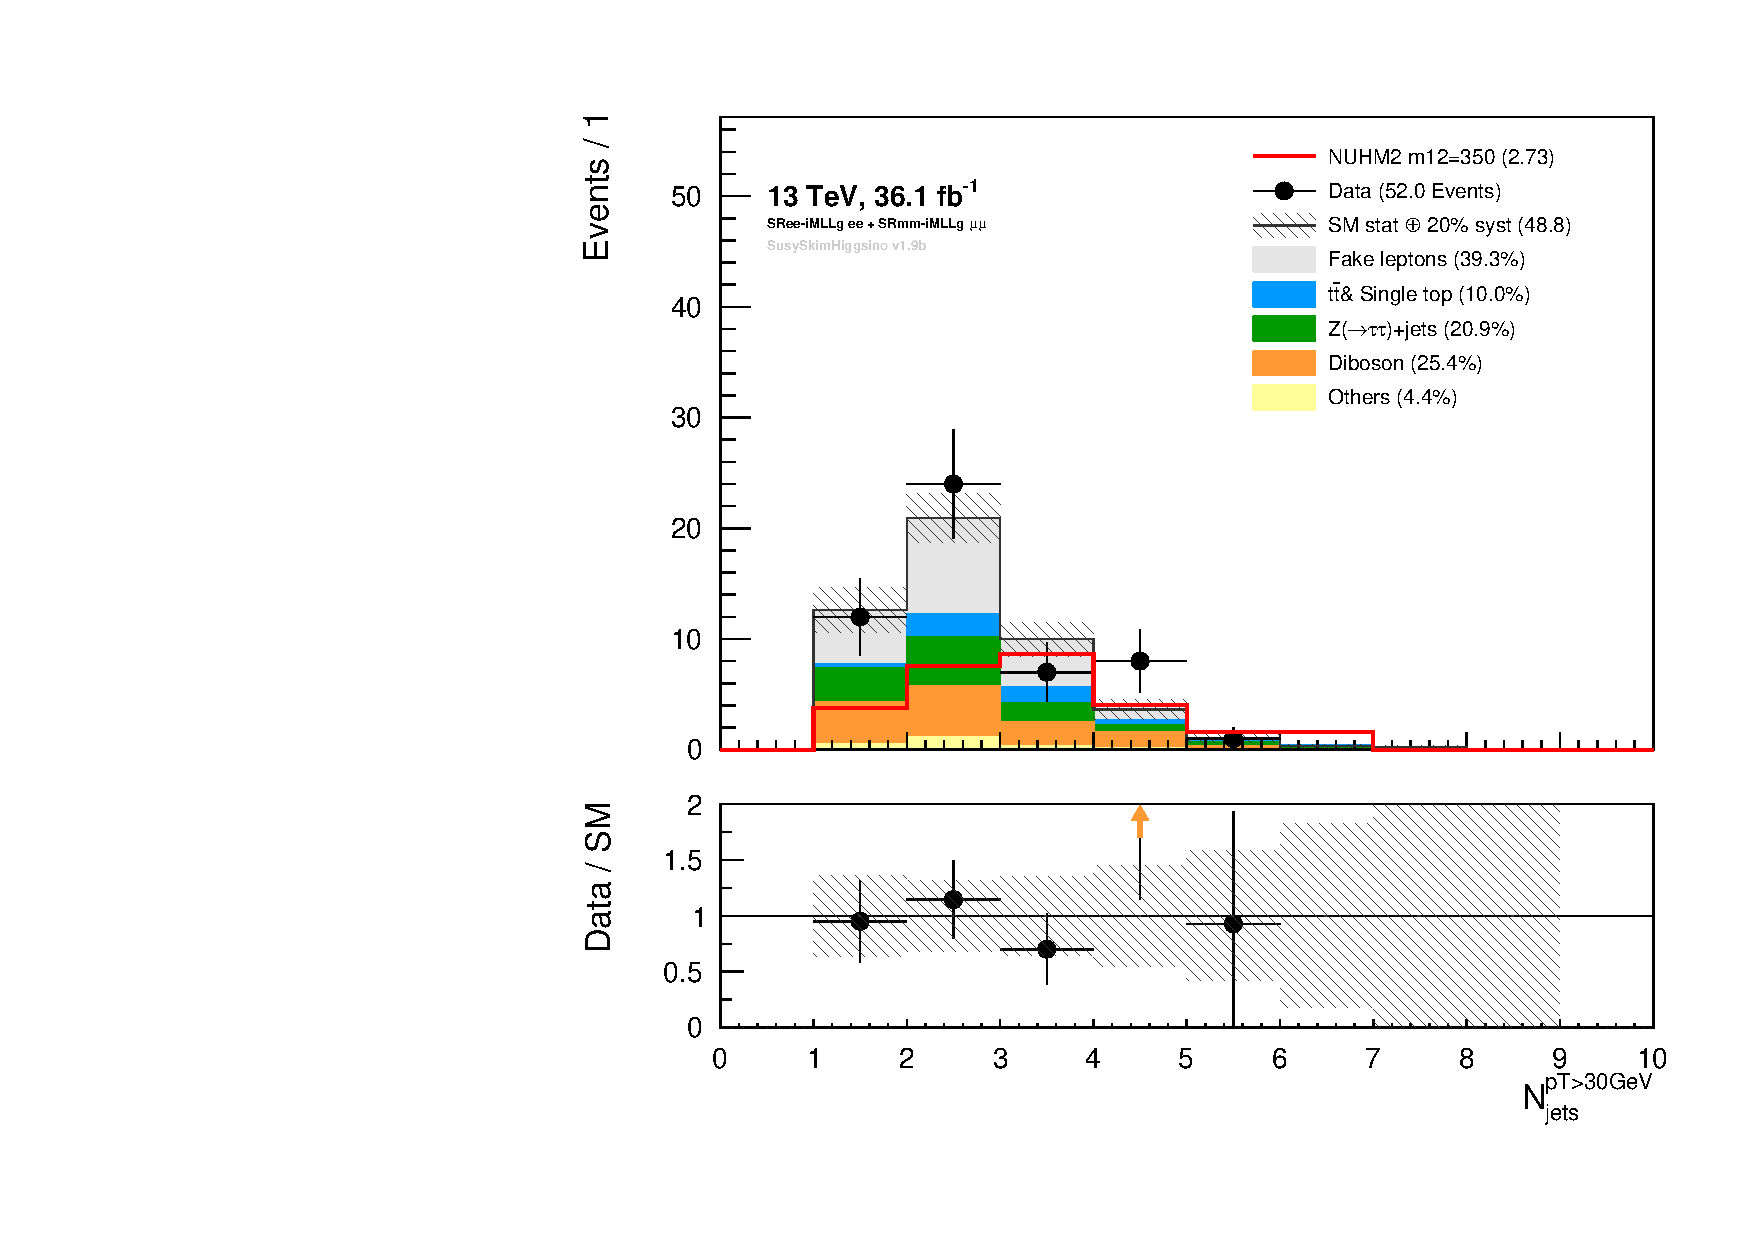
\includegraphics[scale=0.3]{NUHM2_m12_350_and_Bkg_nJet30_SFOS_N_minus_one_distribution_in_SR_times_10_on_Nsig.pdf}
            \caption{$N^{30}_{\mathrm{jets}}$}
            \label{fig:event_nuhm2_m12_350_nJet30_SFOS}
        \end{subfigure}
        \begin{subfigure}[b]{0.48\textwidth}
            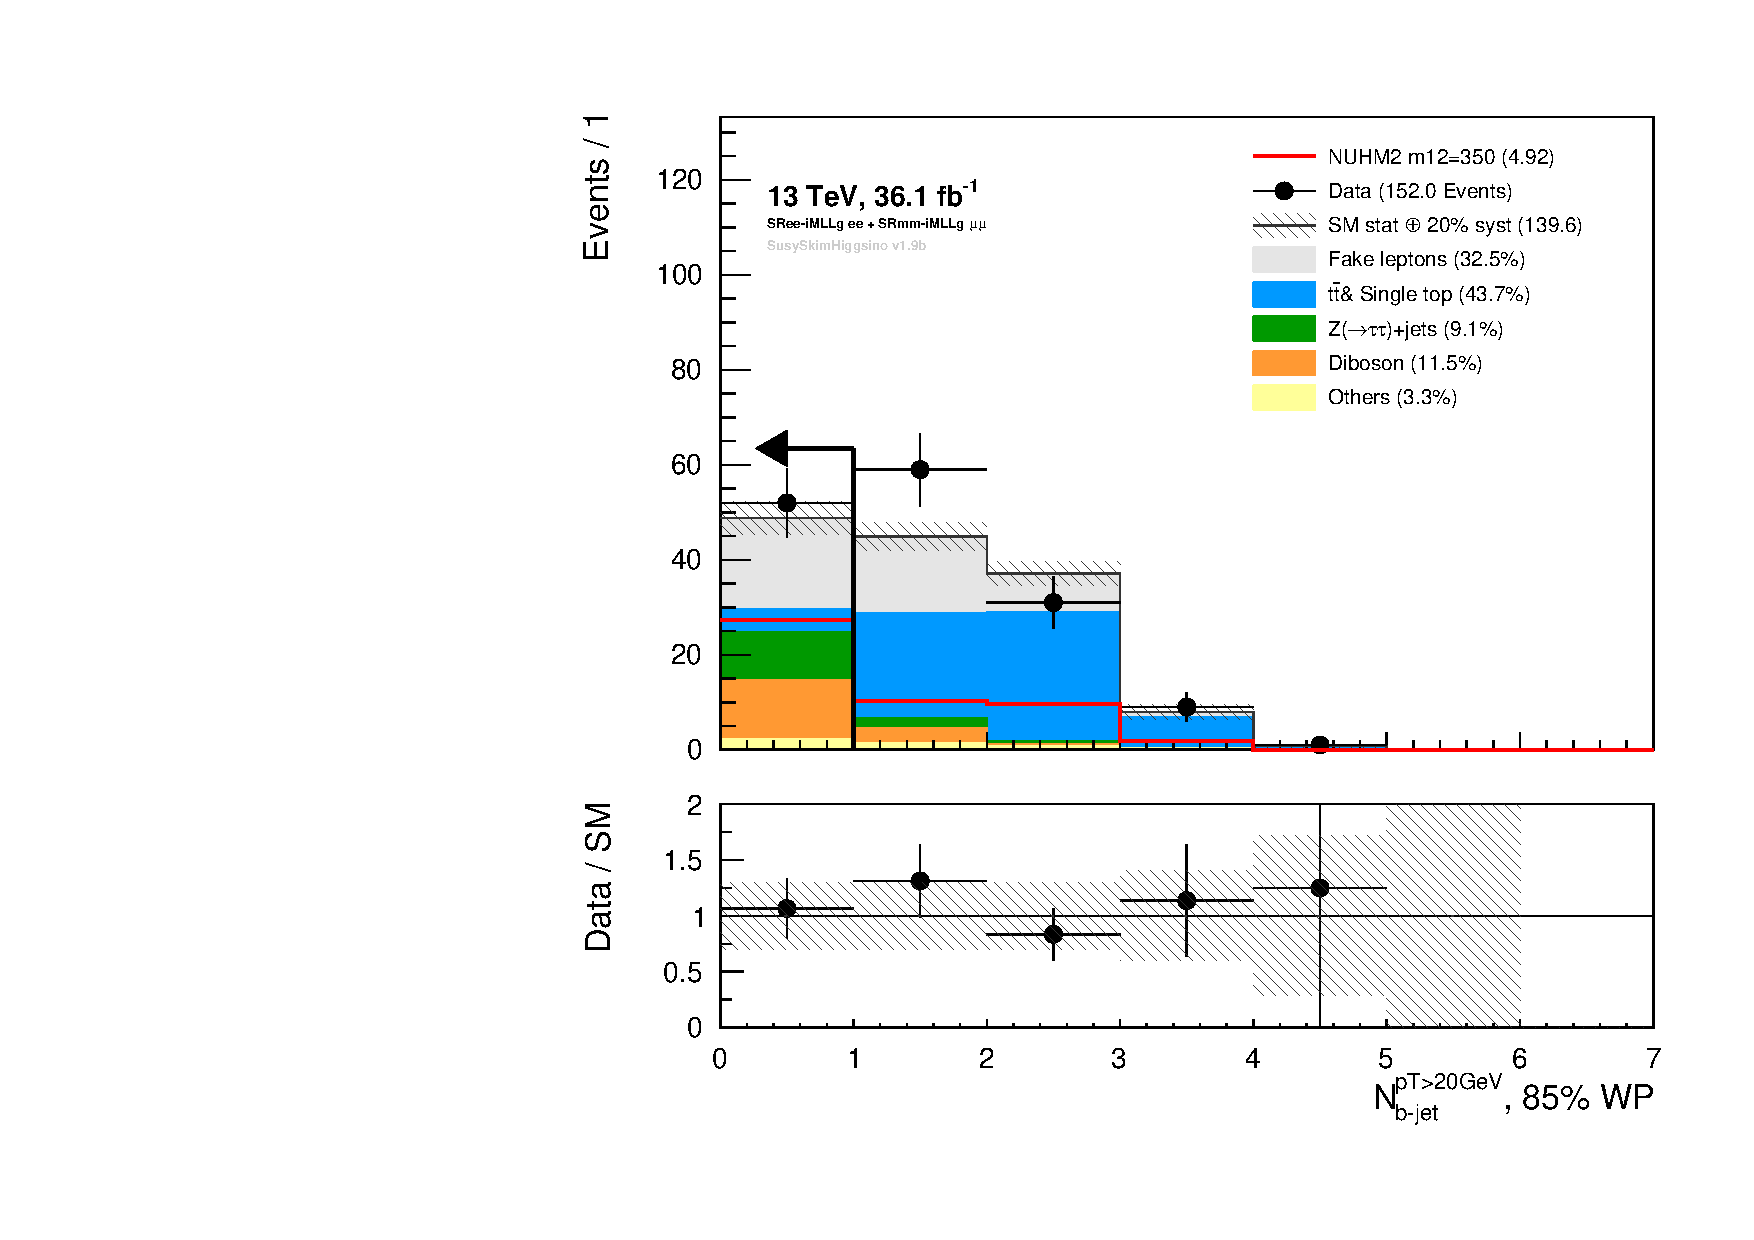
\includegraphics[scale=0.3]{NUHM2_m12_350_and_Bkg_nBJet20_MV2c10_SFOS_N_minus_one_distribution_in_SR_times_10_on_Nsig.pdf}
            \caption{$N^{20}_{\mathrm{b-jets}}$}
            \label{fig:event_nuhm2_m12_350_nBJet20_SFOS}
        \end{subfigure}
        \begin{subfigure}[b]{0.48\textwidth}
            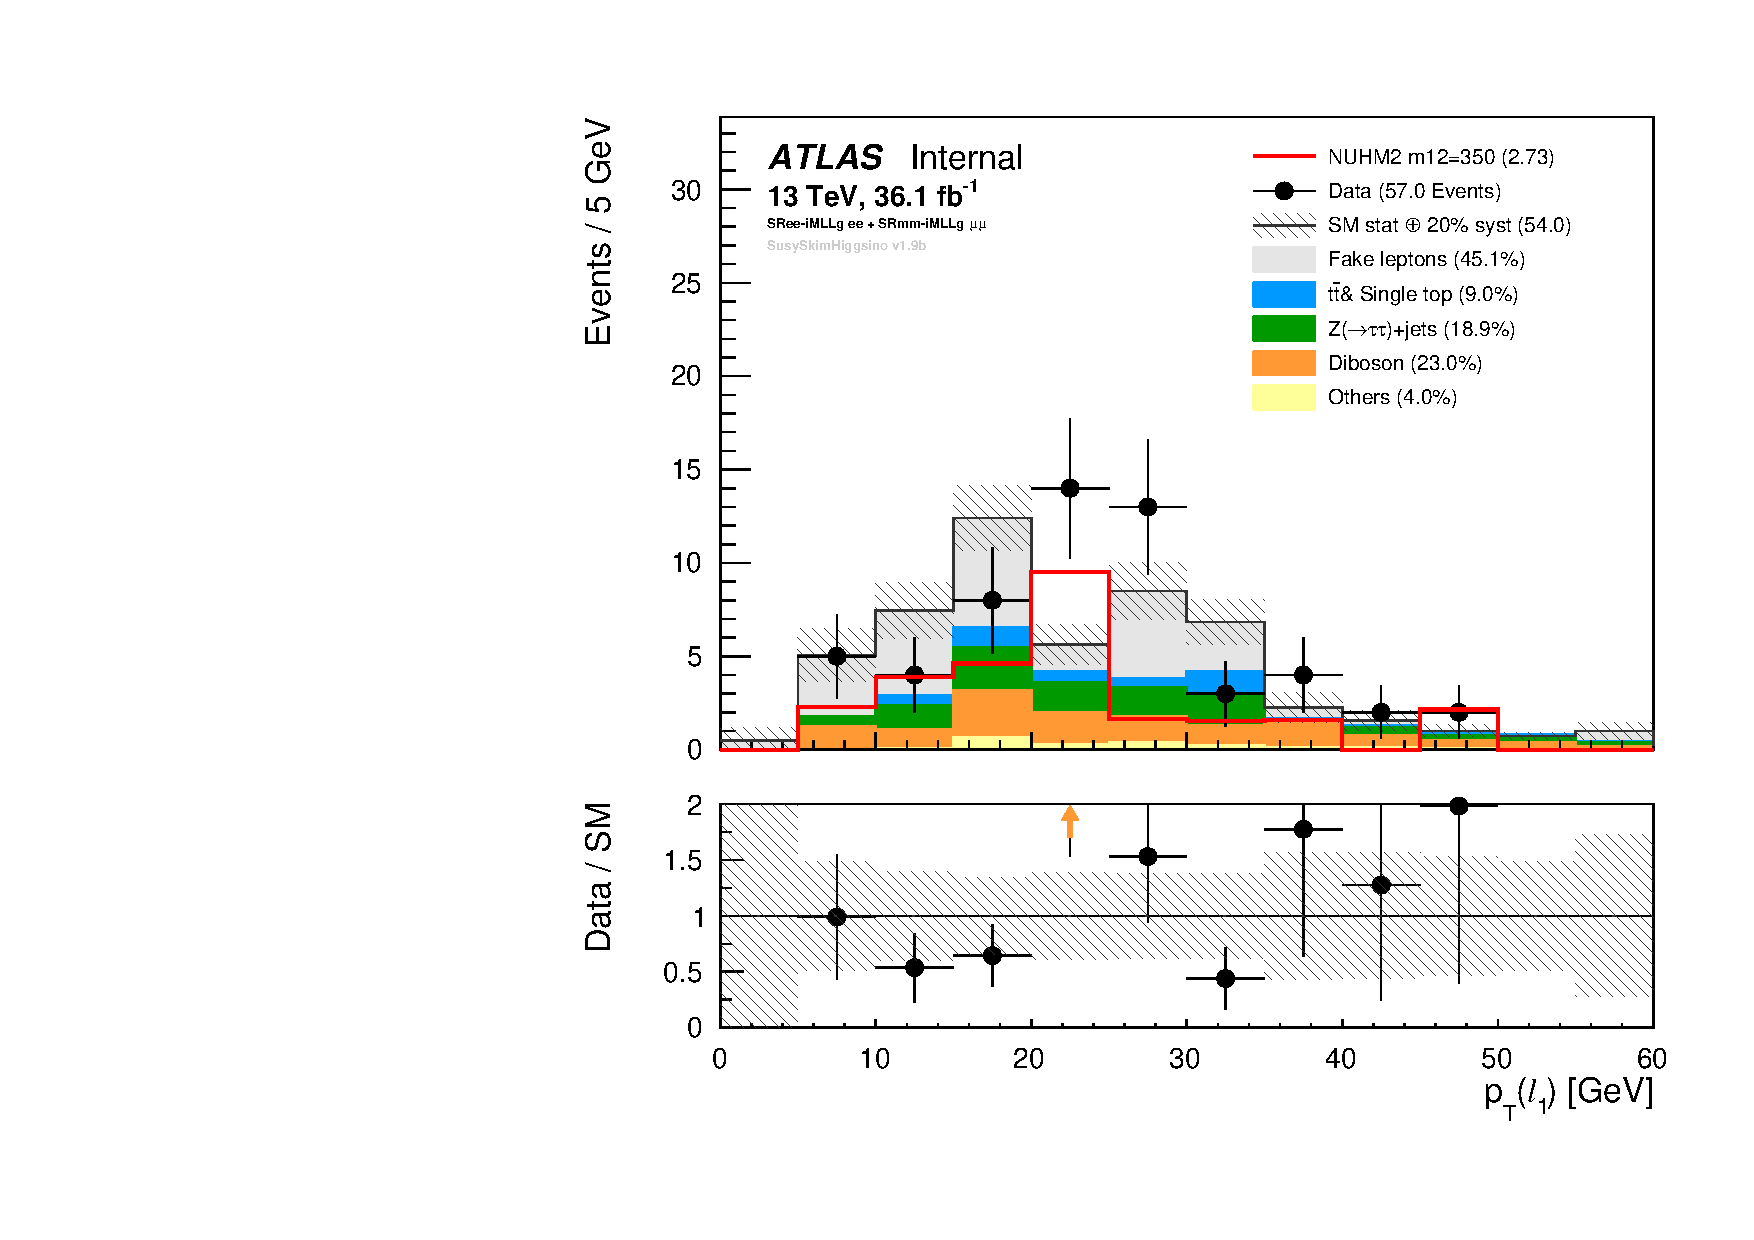
\includegraphics[scale=0.3]{NUHM2_m12_350_and_Bkg_lep1Pt_SFOS_N_minus_one_distribution_in_SR_times_10_on_Nsig.pdf}
            \caption{$p^{\ell_1}_{\mathrm{T}}$}
            \label{fig:event_nuhm2_m12_350_lep1Pt_SFOS}
        \end{subfigure}
        \begin{subfigure}[b]{0.48\textwidth}
            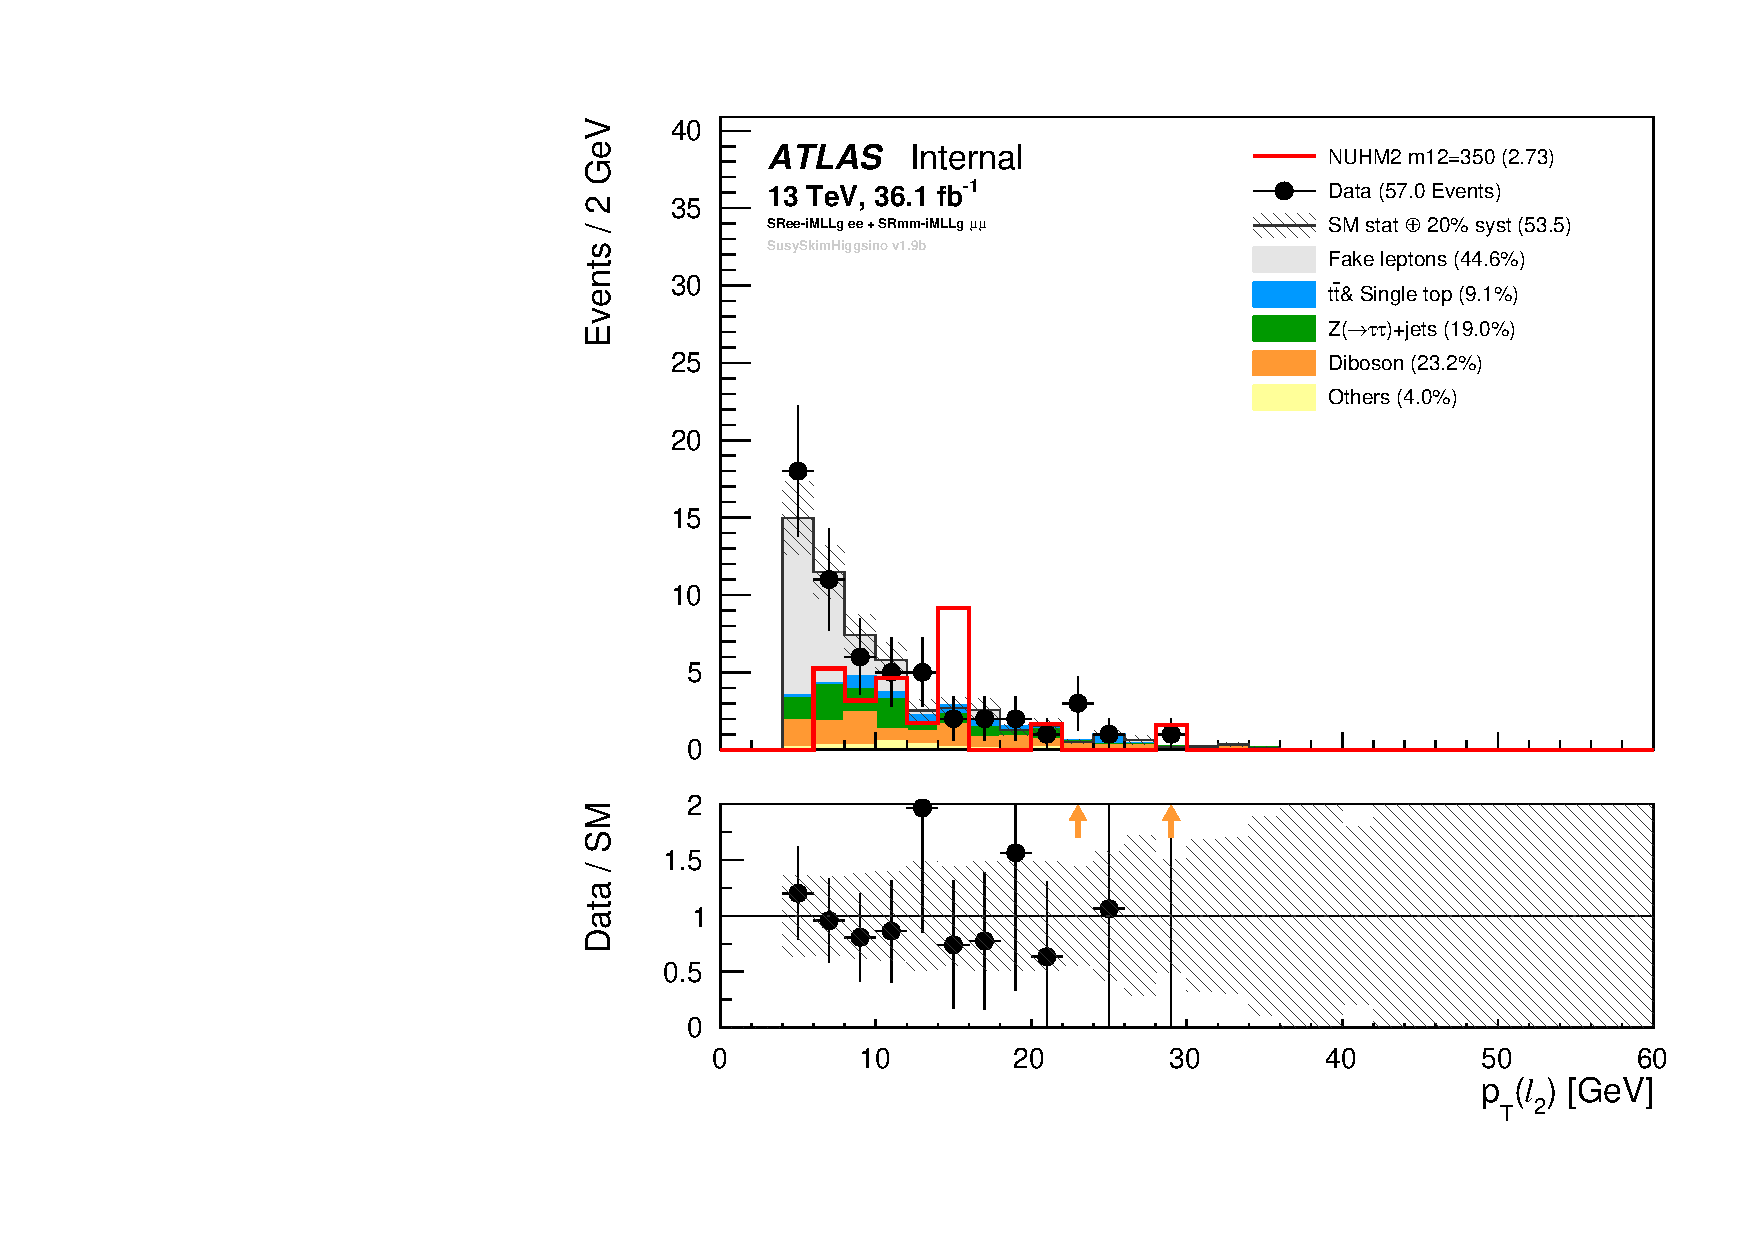
\includegraphics[scale=0.3]{NUHM2_m12_350_and_Bkg_lep2Pt_SFOS_N_minus_one_distribution_in_SR_times_10_on_Nsig.pdf}
            \caption{$p^{\ell_2}_{\mathrm{T}}$}
            \label{fig:event_nuhm2_m12_350_lep2Pt_SFOS}
        \end{subfigure}
        \begin{subfigure}[b]{0.48\textwidth}
            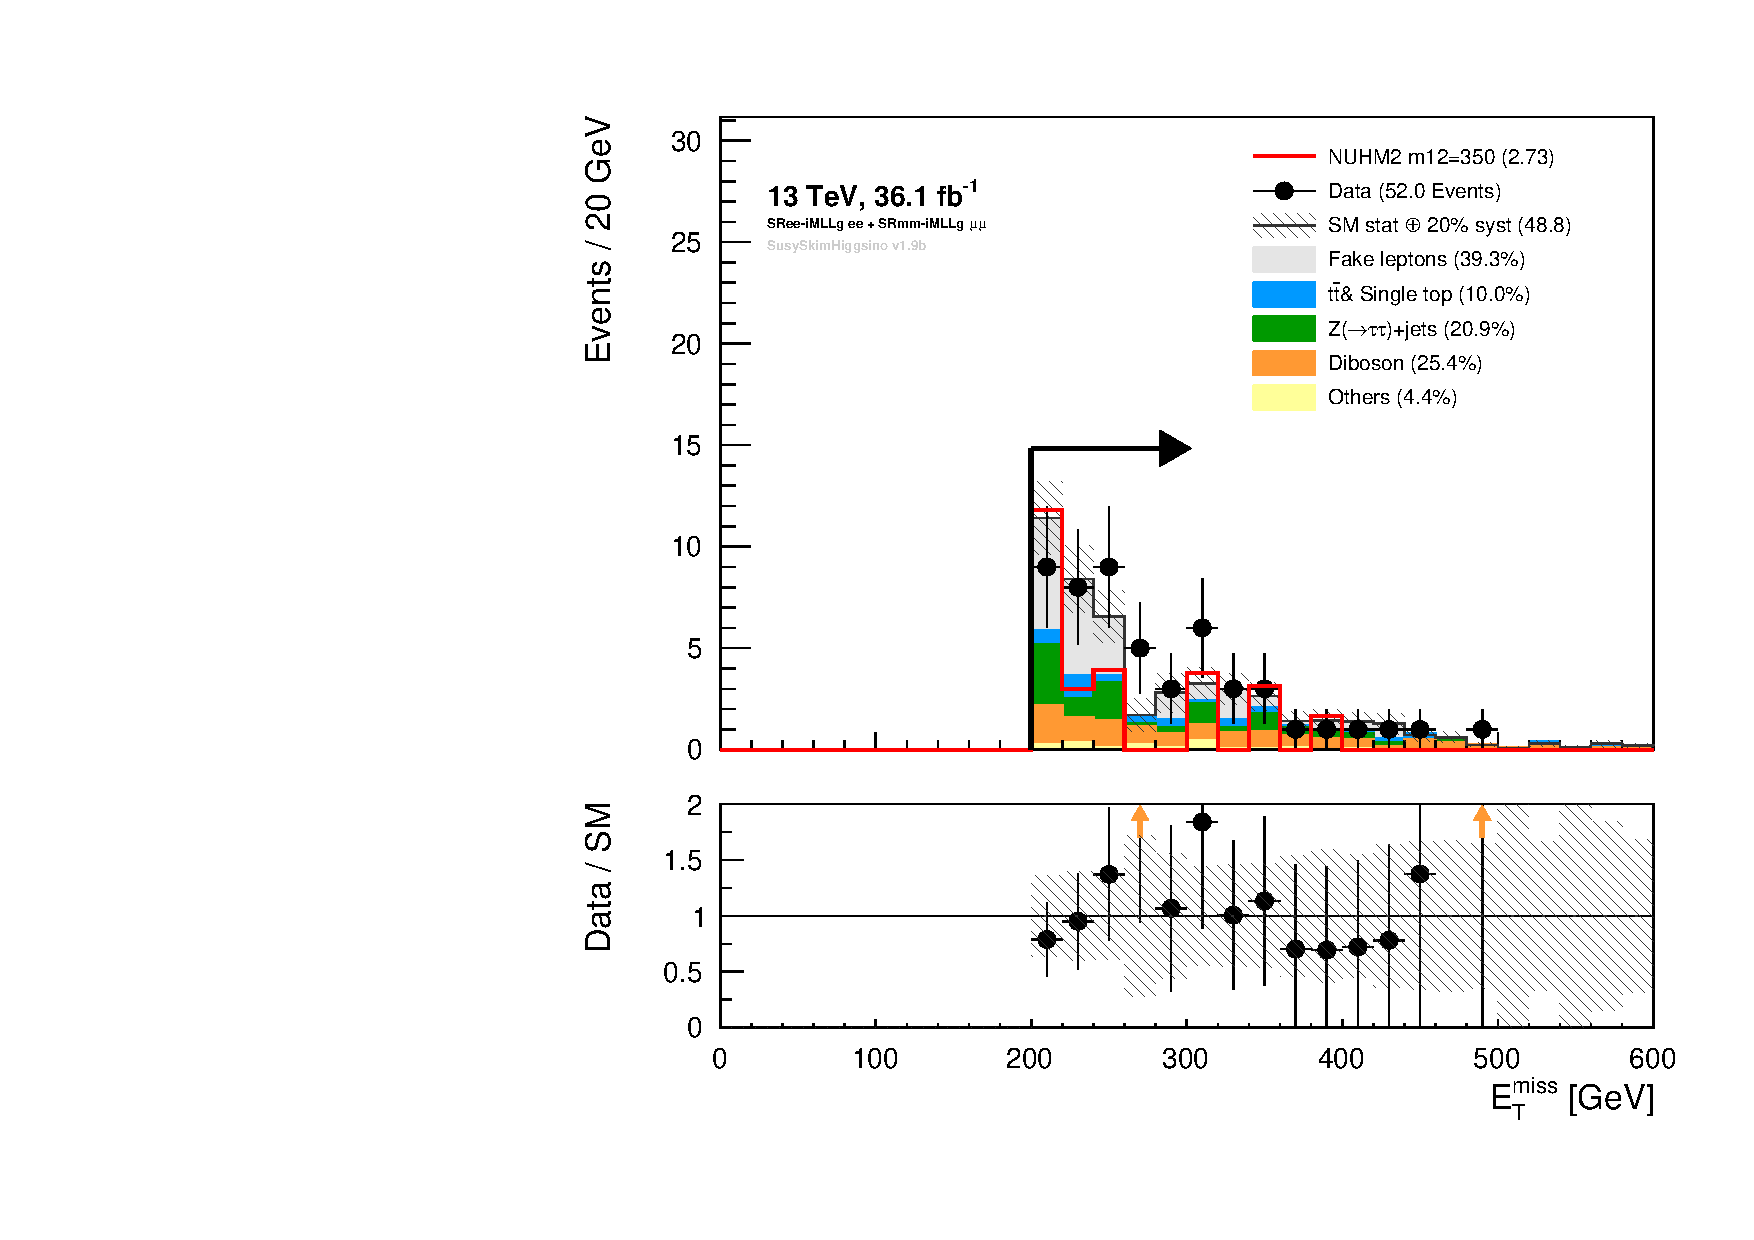
\includegraphics[scale=0.3]{NUHM2_m12_350_and_Bkg_met_Et_SFOS_N_minus_one_distribution_in_SR_times_10_on_Nsig.pdf}
            \caption{$E^{\mathrm{miss}}_{\mathrm{T}}$}
            \label{fig:event_nuhm2_m12_350_met_SFOS}
        \end{subfigure}
        \begin{subfigure}[b]{0.48\textwidth}
            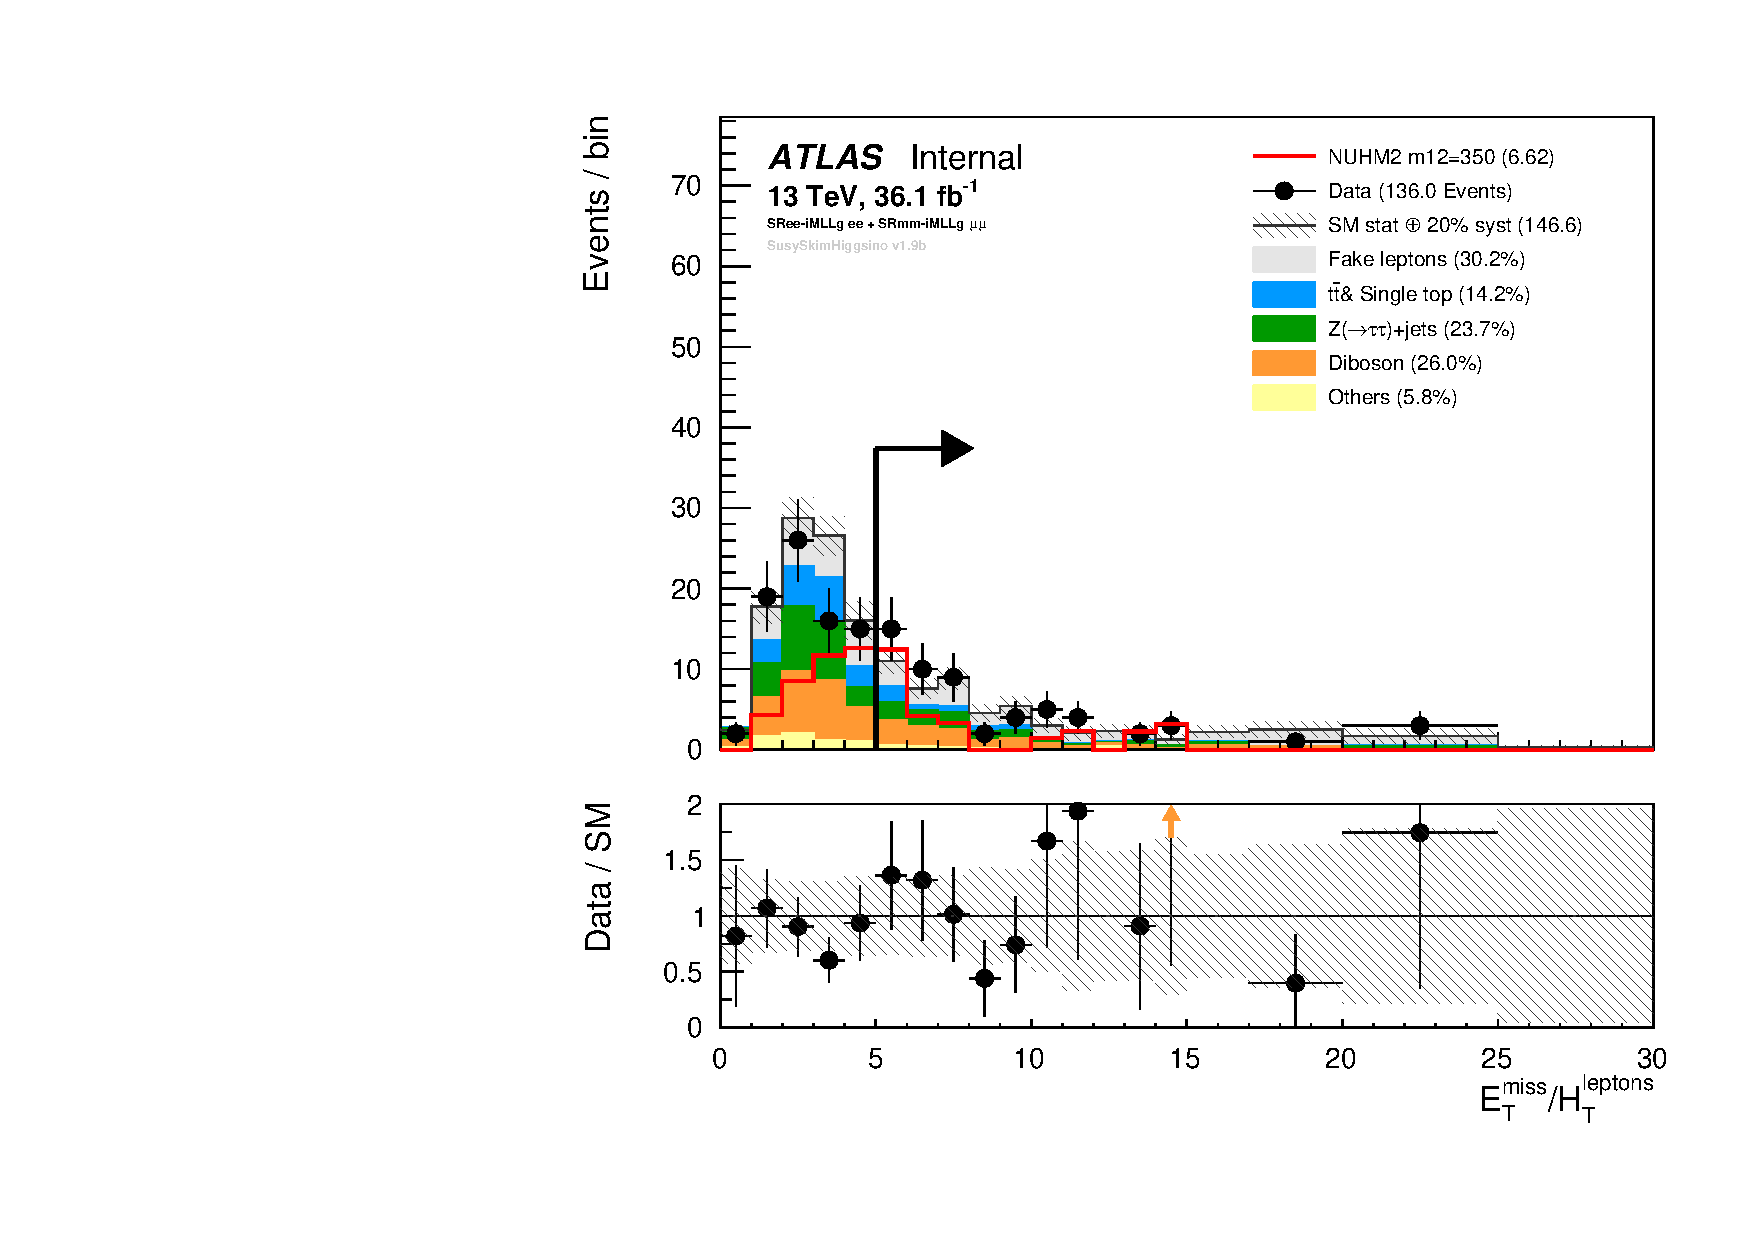
\includegraphics[scale=0.3]{NUHM2_m12_350_and_Bkg_METOverHTLep_SFOS_N_minus_one_distribution_in_SR_times_10_on_Nsig.pdf}
            \caption{$E^{\mathrm{miss}}_{\mathrm{T}} / H^{\mathrm{leptons}}_{\mathrm{T}}$}
            \label{fig:event_nuhm2_m12_350_METOverHTLep_SFOS}
        \end{subfigure}
    \end{center}
    \caption{The `$N-1$' distributions for NUHM2 model with $m_{1/2} = 350$~{\GeV} in SR region $1 < $SR$\ell \ell$-$m_{\ell \ell} < 60$~{\GeV}.
    The NUHM2 distributions are multiplied by 10 but the number of events in the legend use its actual values.}
    \label{fig:dist_nuhm2_kinematic_in_SR_SFOS_m12_350_1}
\end{figure}

\begin{figure}[htbp]
    \begin{center}
        \begin{subfigure}[b]{0.48\textwidth}
            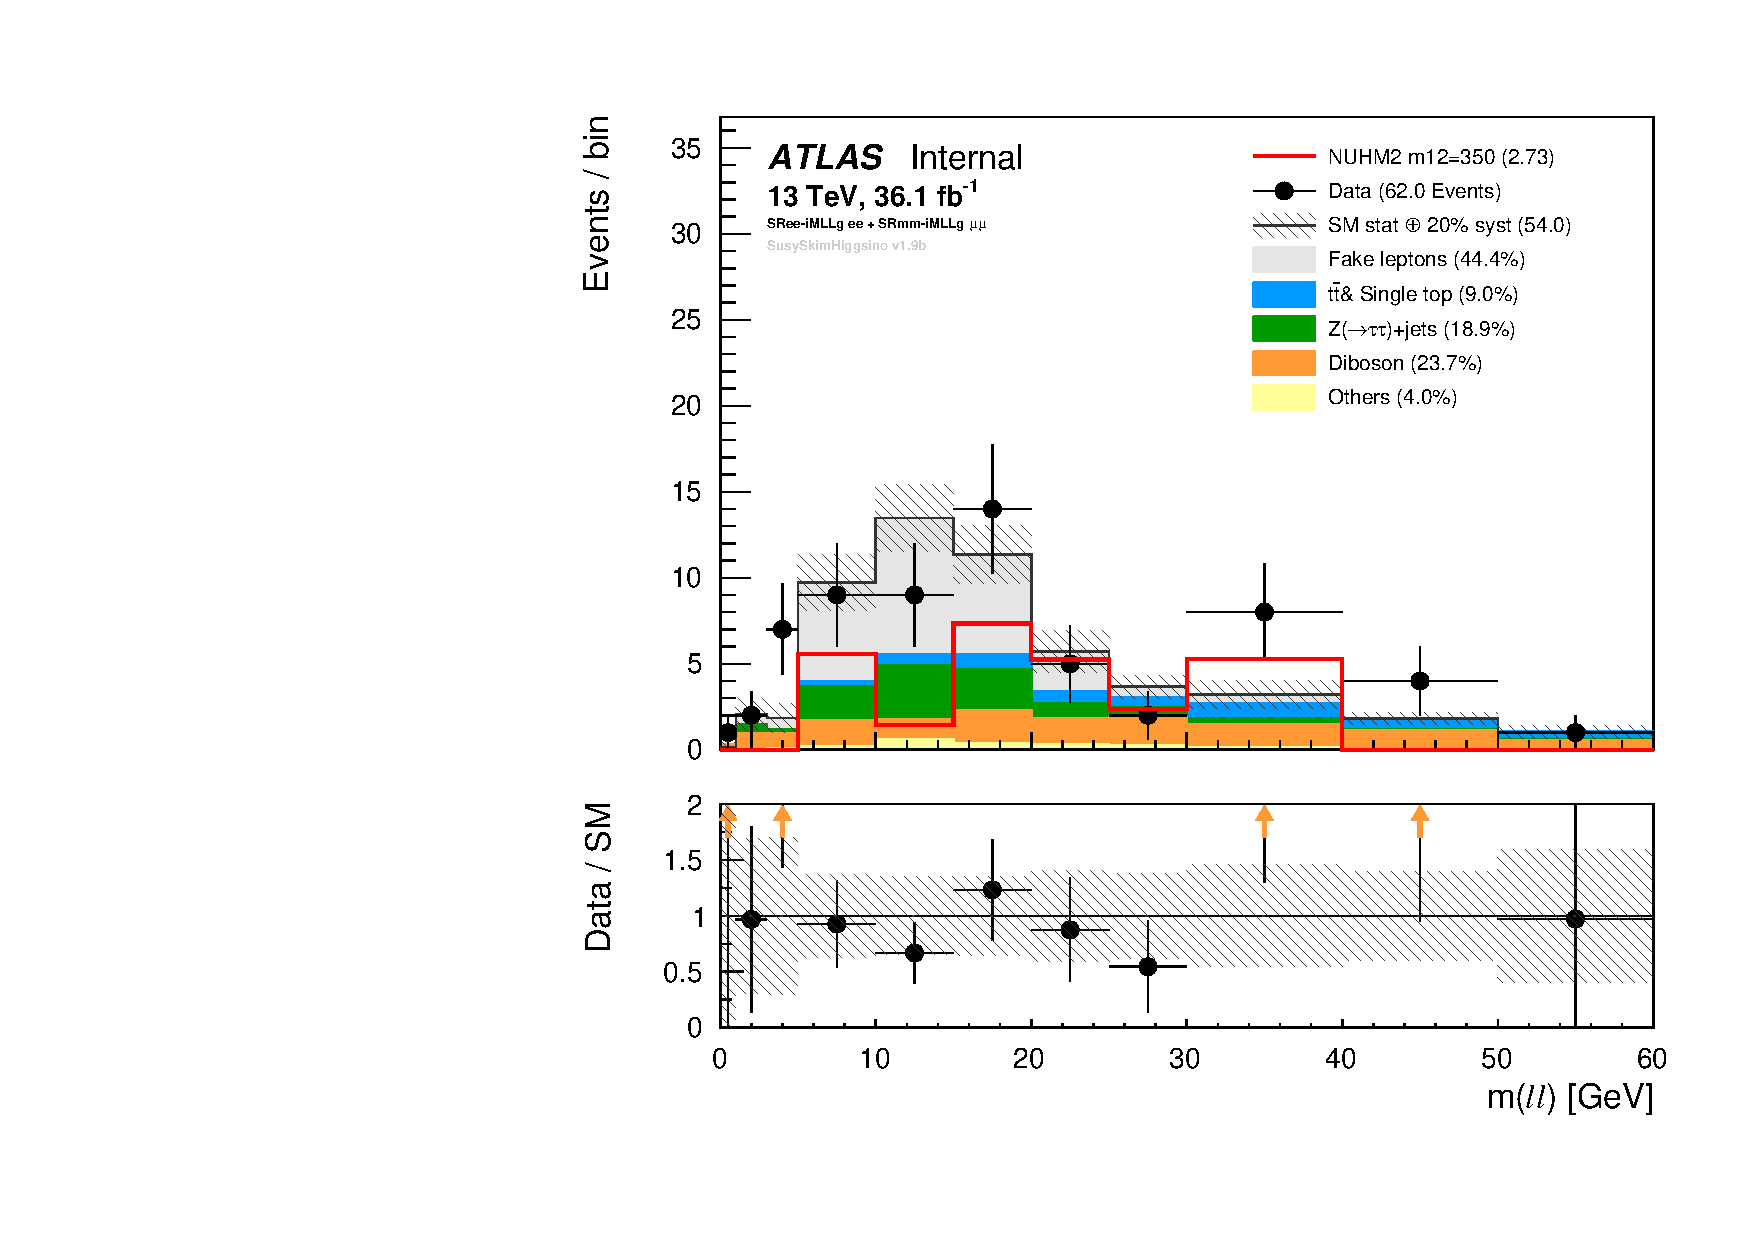
\includegraphics[scale=0.3]{NUHM2_m12_350_and_Bkg_mll_SFOS_N_minus_one_distribution_in_SR_times_10_on_Nsig.pdf}
            \caption{$m_{\ell\ell}$}
            \label{fig:event_nuhm2_m12_350_mll_SFOS}
        \end{subfigure}
        \begin{subfigure}[b]{0.48\textwidth}
            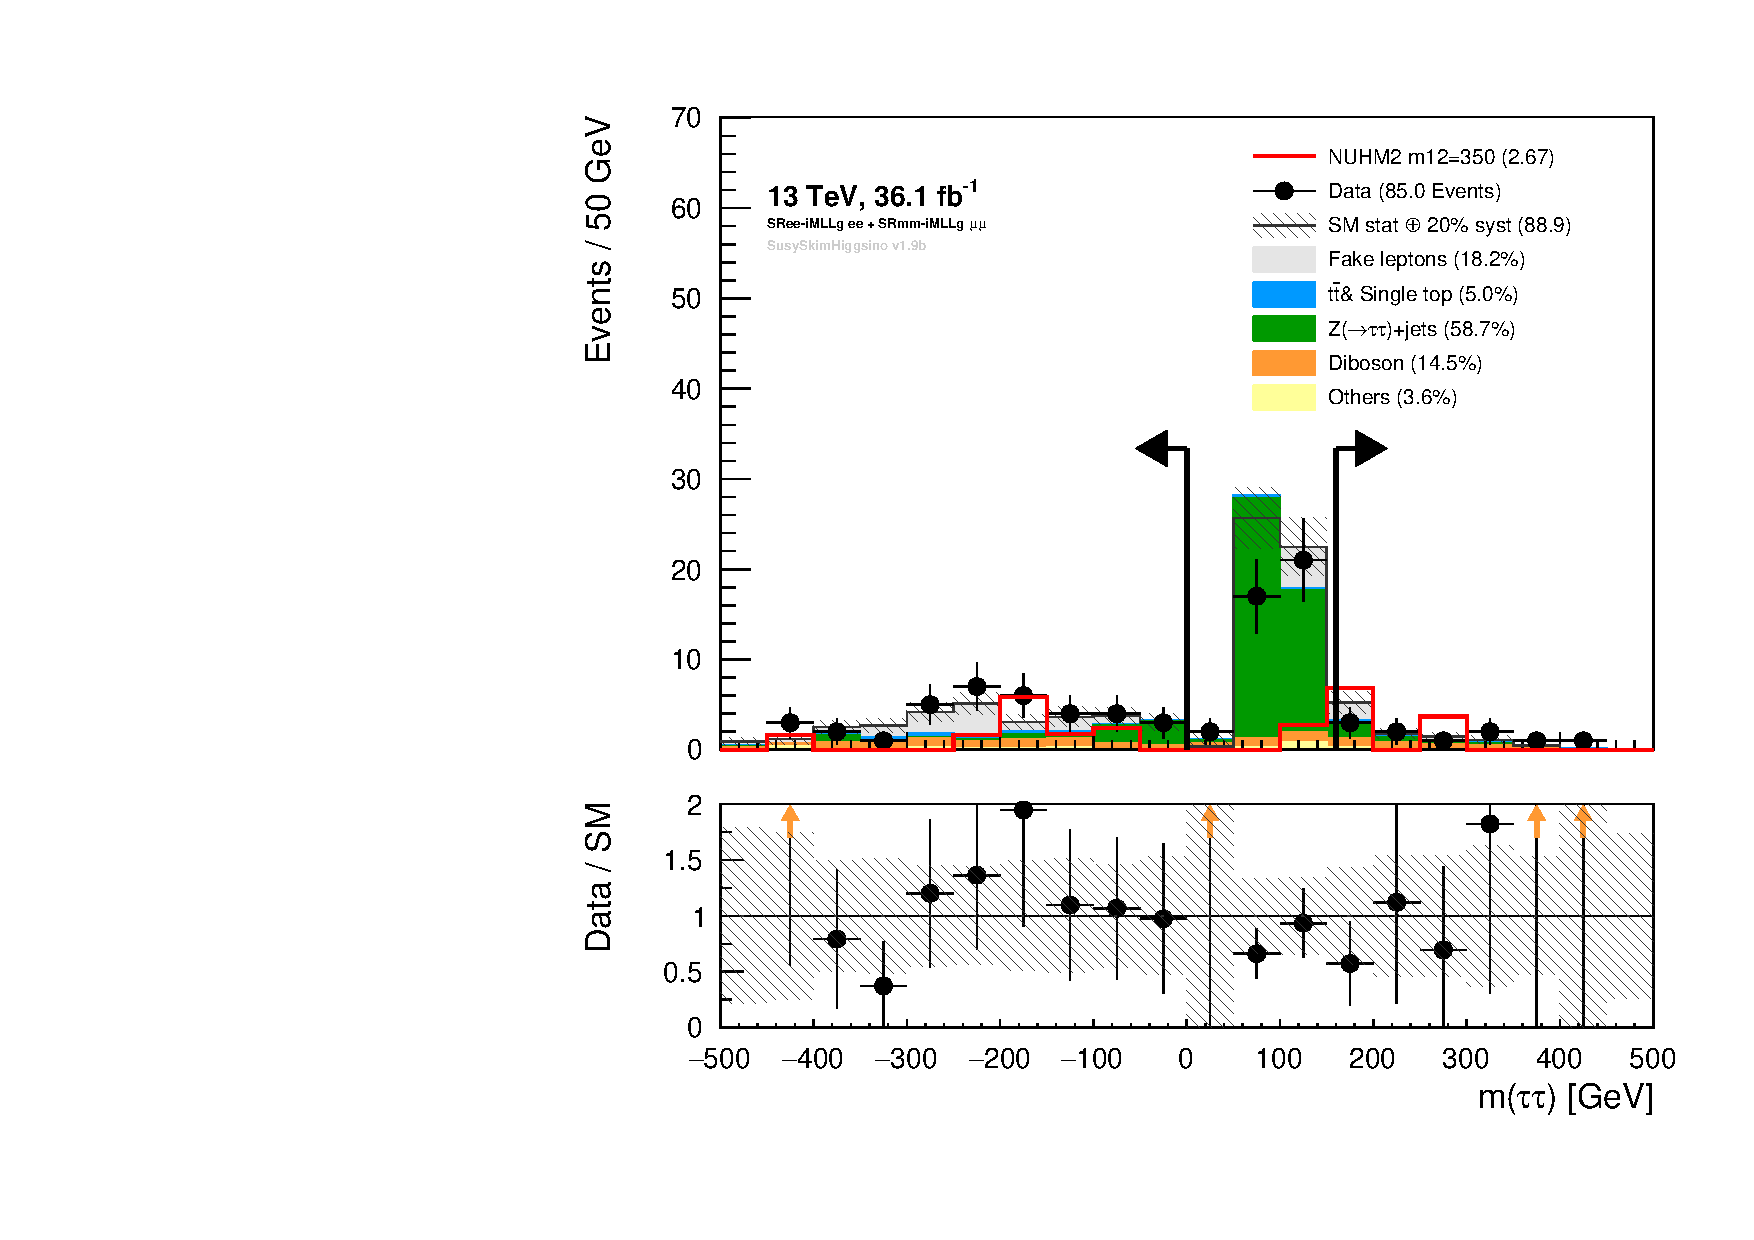
\includegraphics[scale=0.3]{NUHM2_m12_350_and_Bkg_MTauTau_SFOS_N_minus_one_distribution_in_SR_times_10_on_Nsig.pdf}
            \caption{$m_{\tau\tau}$}
            \label{fig:event_nuhm2_m12_350_MTauTau_SFOS}
        \end{subfigure}
        \begin{subfigure}[b]{0.48\textwidth}
            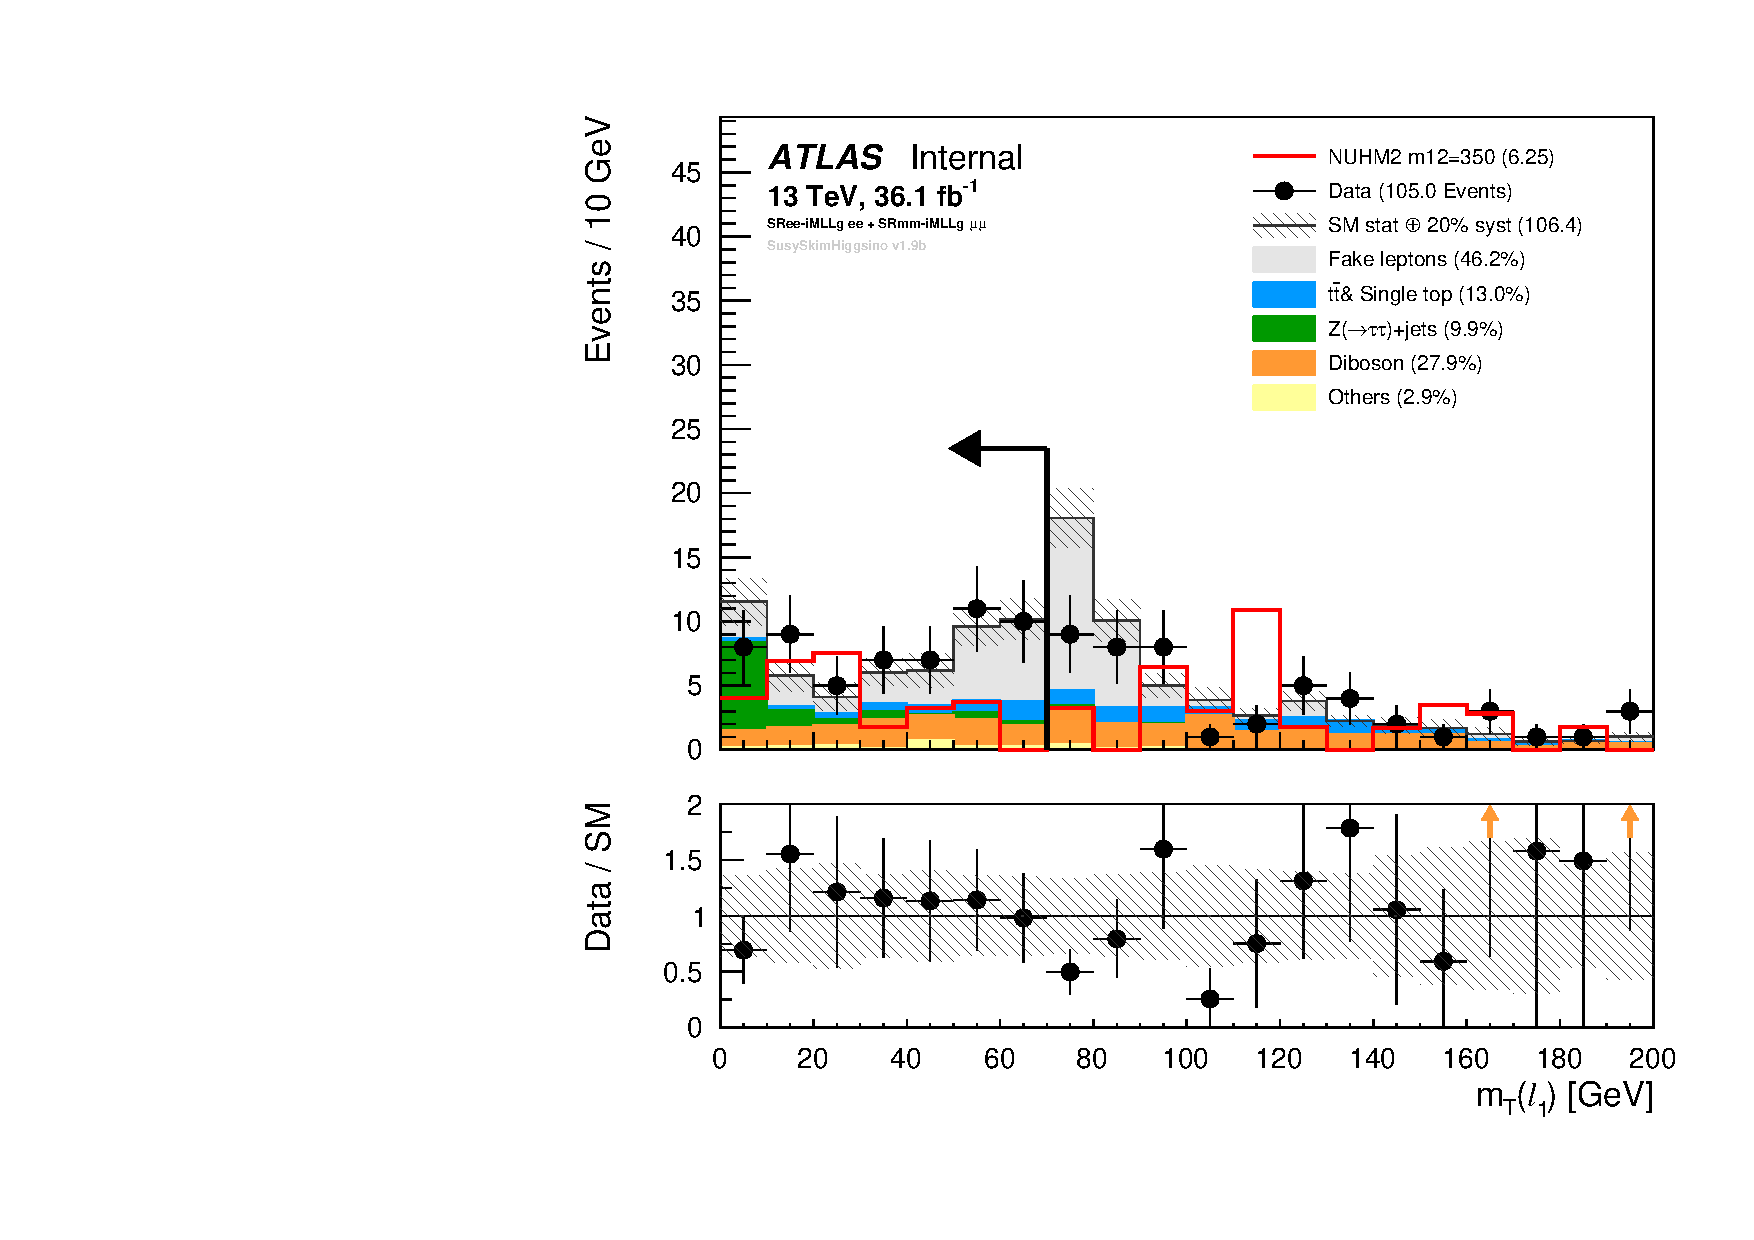
\includegraphics[scale=0.3]{NUHM2_m12_350_and_Bkg_mt_lep1_SFOS_N_minus_one_distribution_in_SR_times_10_on_Nsig.pdf}
            \caption{$m_{T}(\ell_{1})$}
            \label{fig:event_nuhm2_m12_350_mt_lep1_SFOS}
        \end{subfigure}
        \begin{subfigure}[b]{0.48\textwidth}
            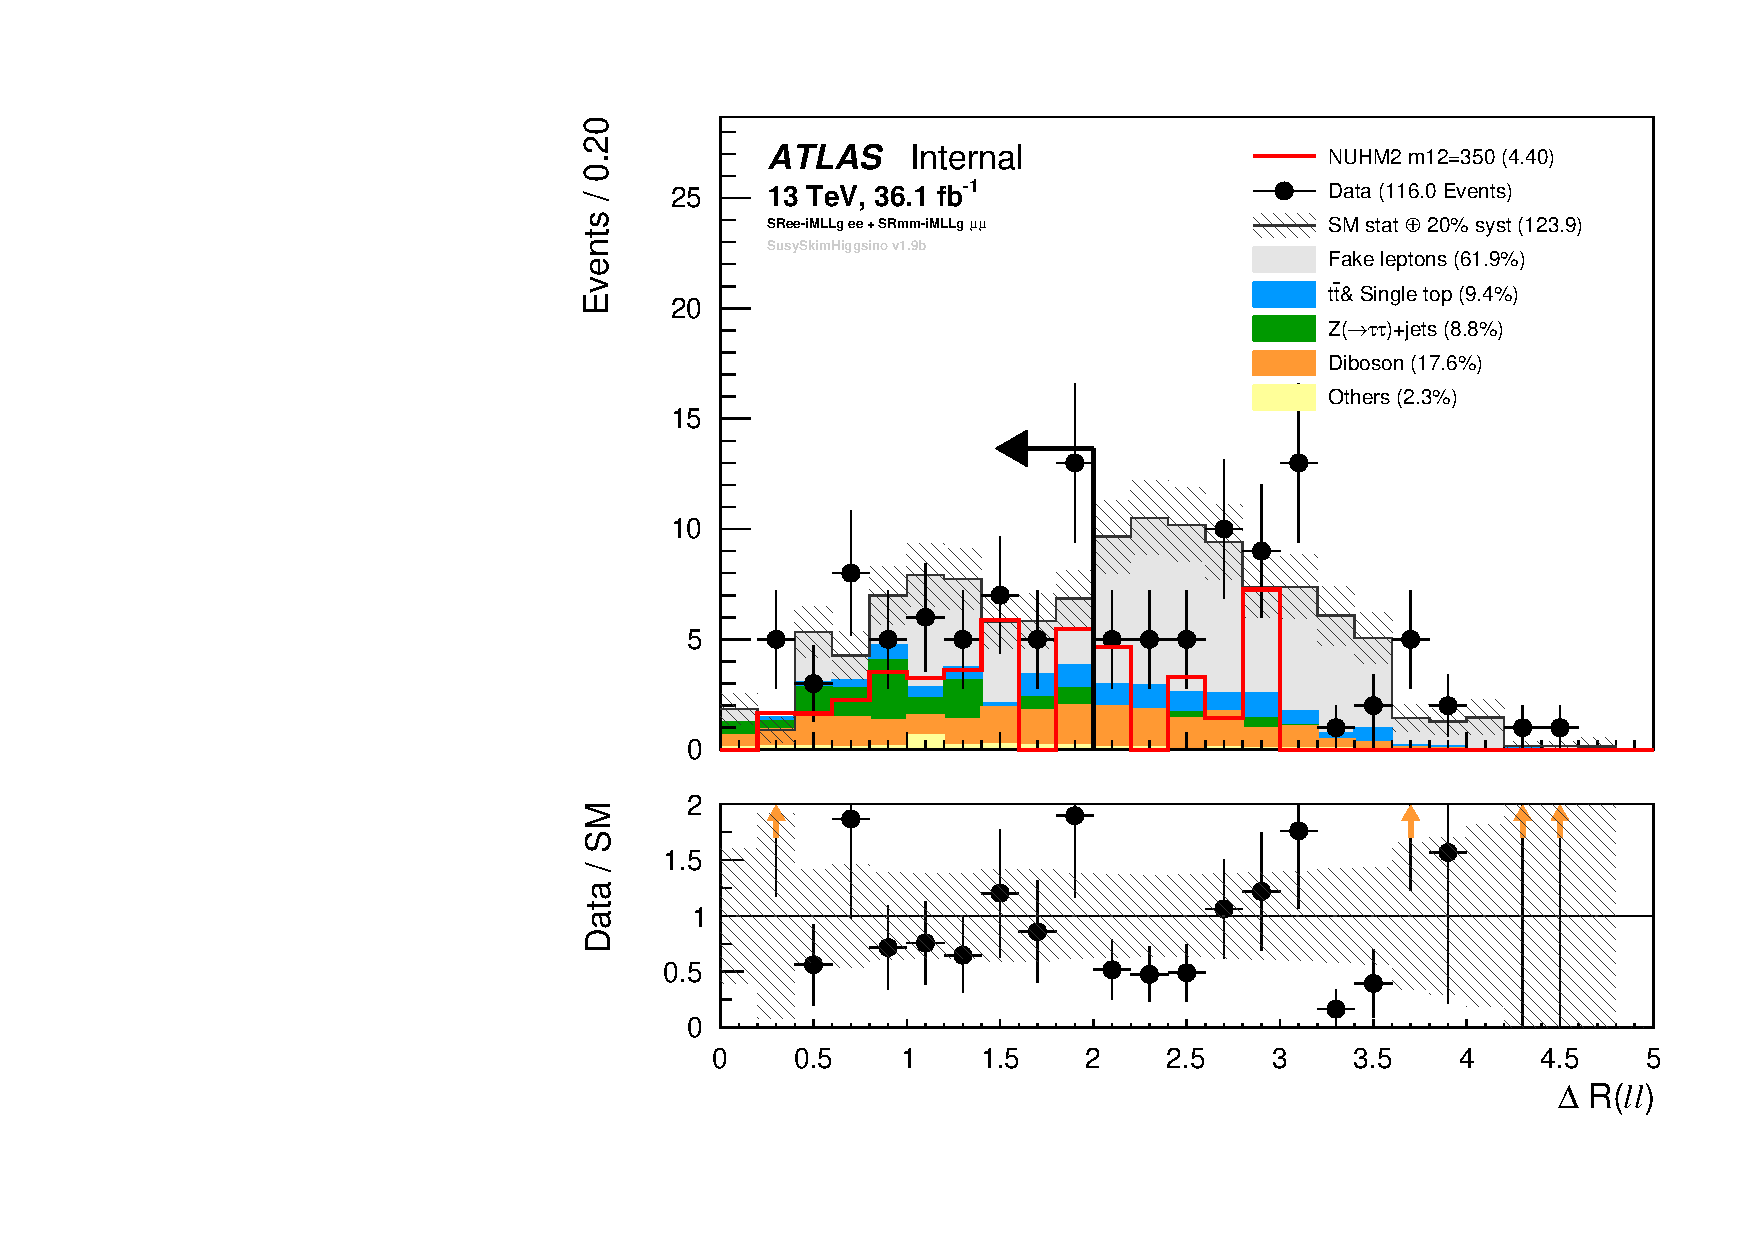
\includegraphics[scale=0.3]{NUHM2_m12_350_and_Bkg_Rll_SFOS_N_minus_one_distribution_in_SR_times_10_on_Nsig.pdf}
            \caption{$\Delta R_{\ell\ell}$}
            \label{fig:event_nuhm2_m12_350_Rll_SFOS}
        \end{subfigure}
        \begin{subfigure}[b]{0.48\textwidth}
            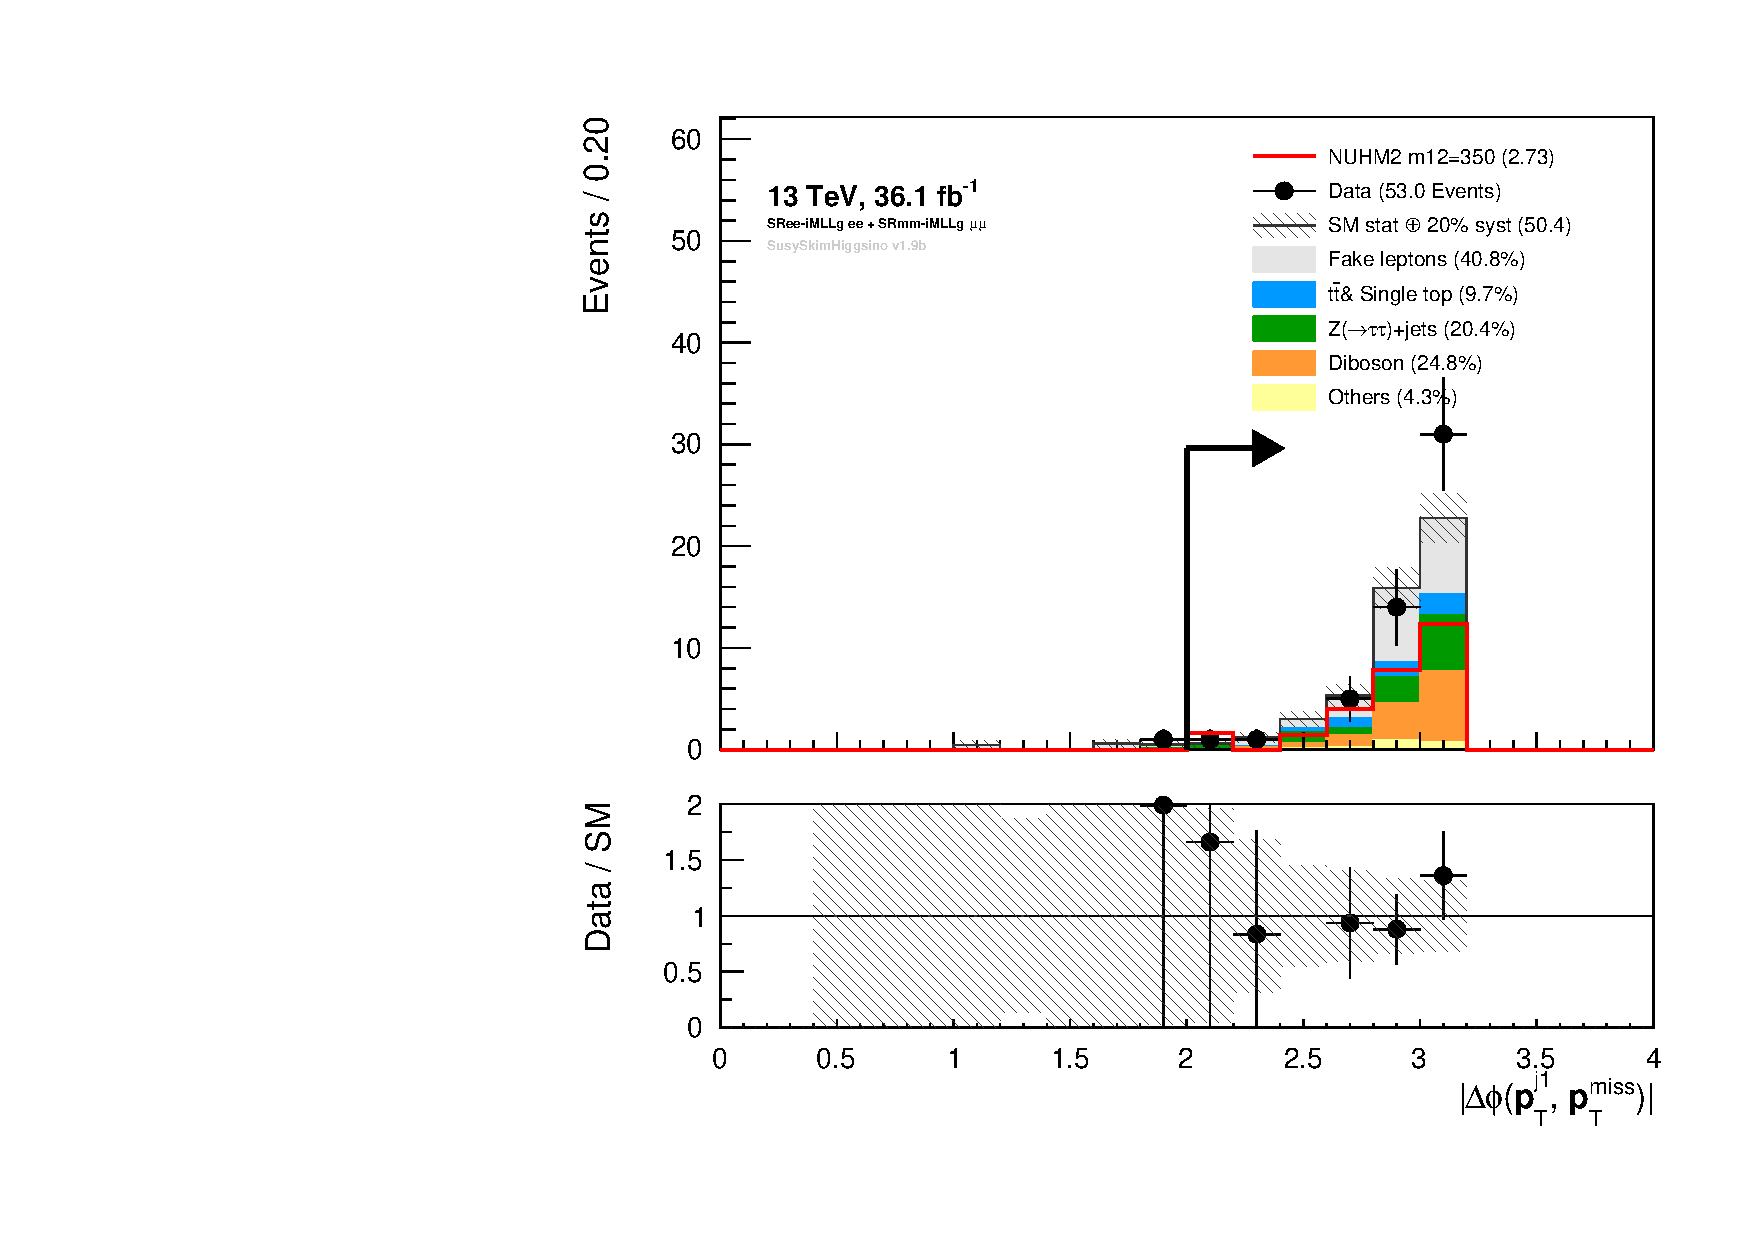
\includegraphics[scale=0.3]{NUHM2_m12_350_and_Bkg_DPhiJ1Met_SFOS_N_minus_one_distribution_in_SR_times_10_on_Nsig.pdf}
            \caption{$|\Delta \phi(\mathbf{p}^{j_{1}}_{\mathrm{T}}, \mathbf{p}^{\mathrm{miss}}_{\mathrm{T}})|$}
            \label{fig:event_nuhm2_m12_350_DPhiJ1Met_SFOS}
        \end{subfigure}
        \begin{subfigure}[b]{0.48\textwidth}
            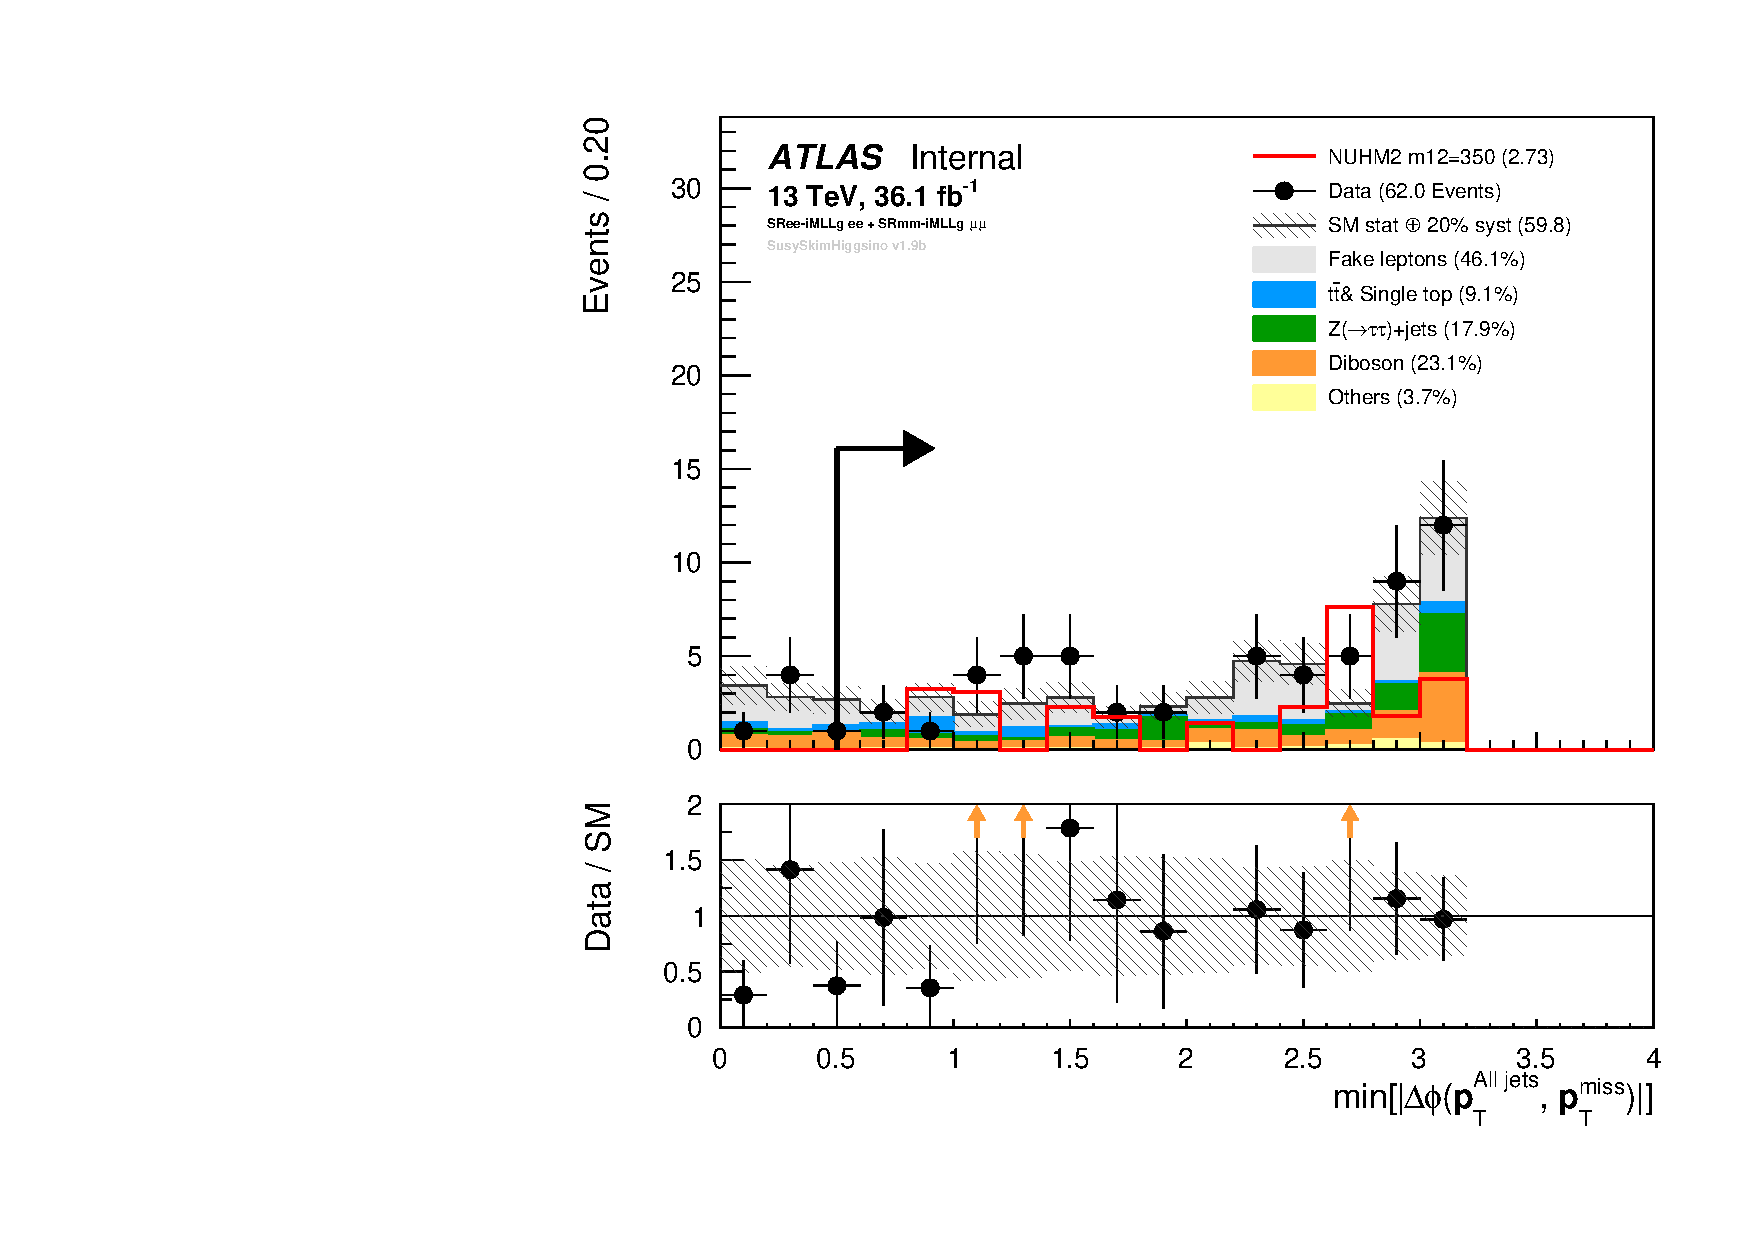
\includegraphics[scale=0.3]{NUHM2_m12_350_and_Bkg_minDPhiAllJetsMet_SFOS_N_minus_one_distribution_in_SR_times_10_on_Nsig.pdf}
            \caption{min[$|\Delta \phi(\mathbf{p}^{\textrm{All jets}}_{\mathrm{T}}, \mathbf{p}^{\mathrm{miss}}_{\mathrm{T}})|$]}
            \label{fig:event_nuhm2_m12_350_minDPhiAllJetsMet_SFOS}
        \end{subfigure}
    \end{center}
    \caption{The `$N-1$' distributions for NUHM2 model with $m_{1/2} = 350$~{\GeV} in SR region $1 < $SR$\ell \ell$-$m_{\ell \ell} < 60$~{\GeV}.
    The NUHM2 distributions are multiplied by 10 but the number of events in the legend use its actual values.}
    \label{fig:dist_nuhm2_kinematic_in_SR_SFOS_m12_350_2}
\end{figure}

% m12 = 400
\begin{figure}[htbp]
    \begin{center}
        \begin{subfigure}[b]{0.48\textwidth}
            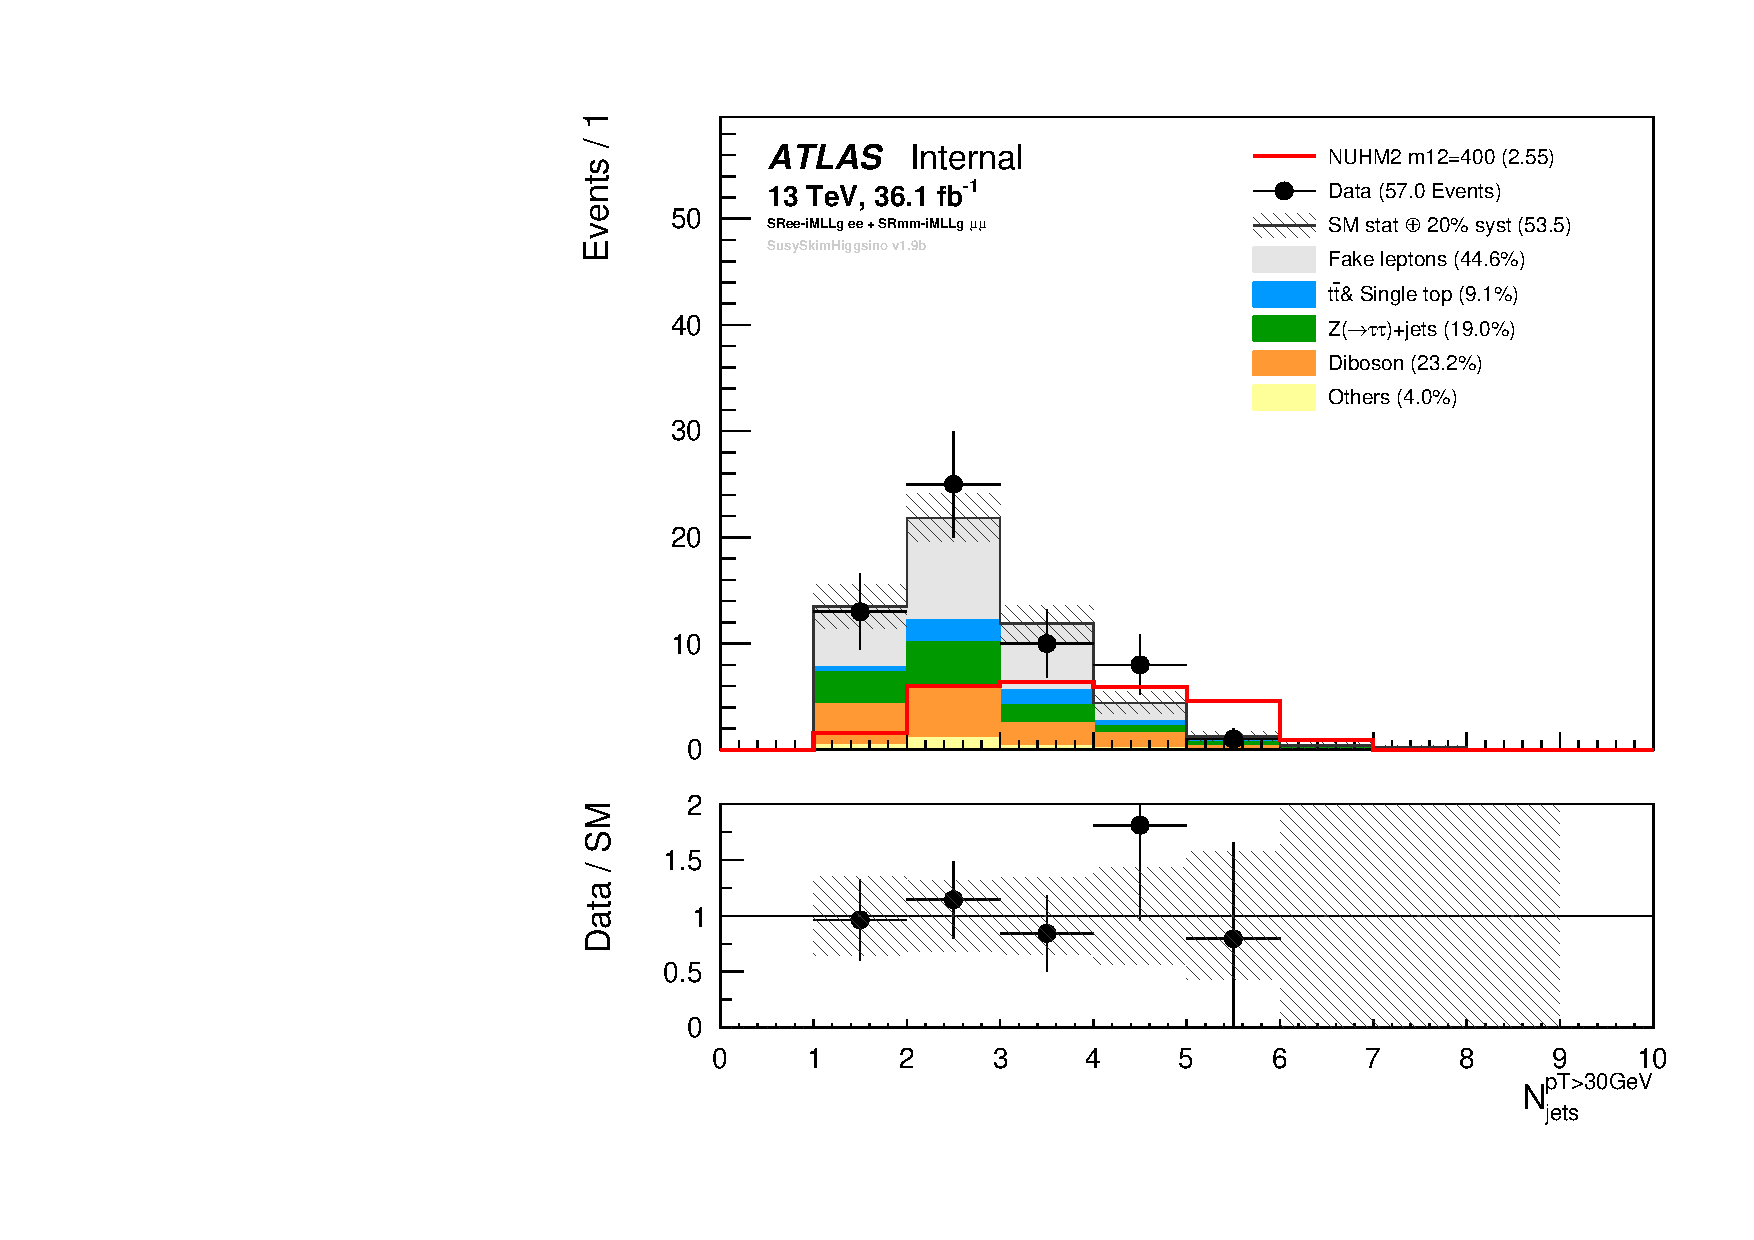
\includegraphics[scale=0.3]{NUHM2_m12_400_and_Bkg_nJet30_SFOS_N_minus_one_distribution_in_SR_times_10_on_Nsig.pdf}
            \caption{$N^{30}_{\mathrm{jets}}$}
            \label{fig:event_nuhm2_m12_400_nJet30_SFOS}
        \end{subfigure}
        \begin{subfigure}[b]{0.48\textwidth}
            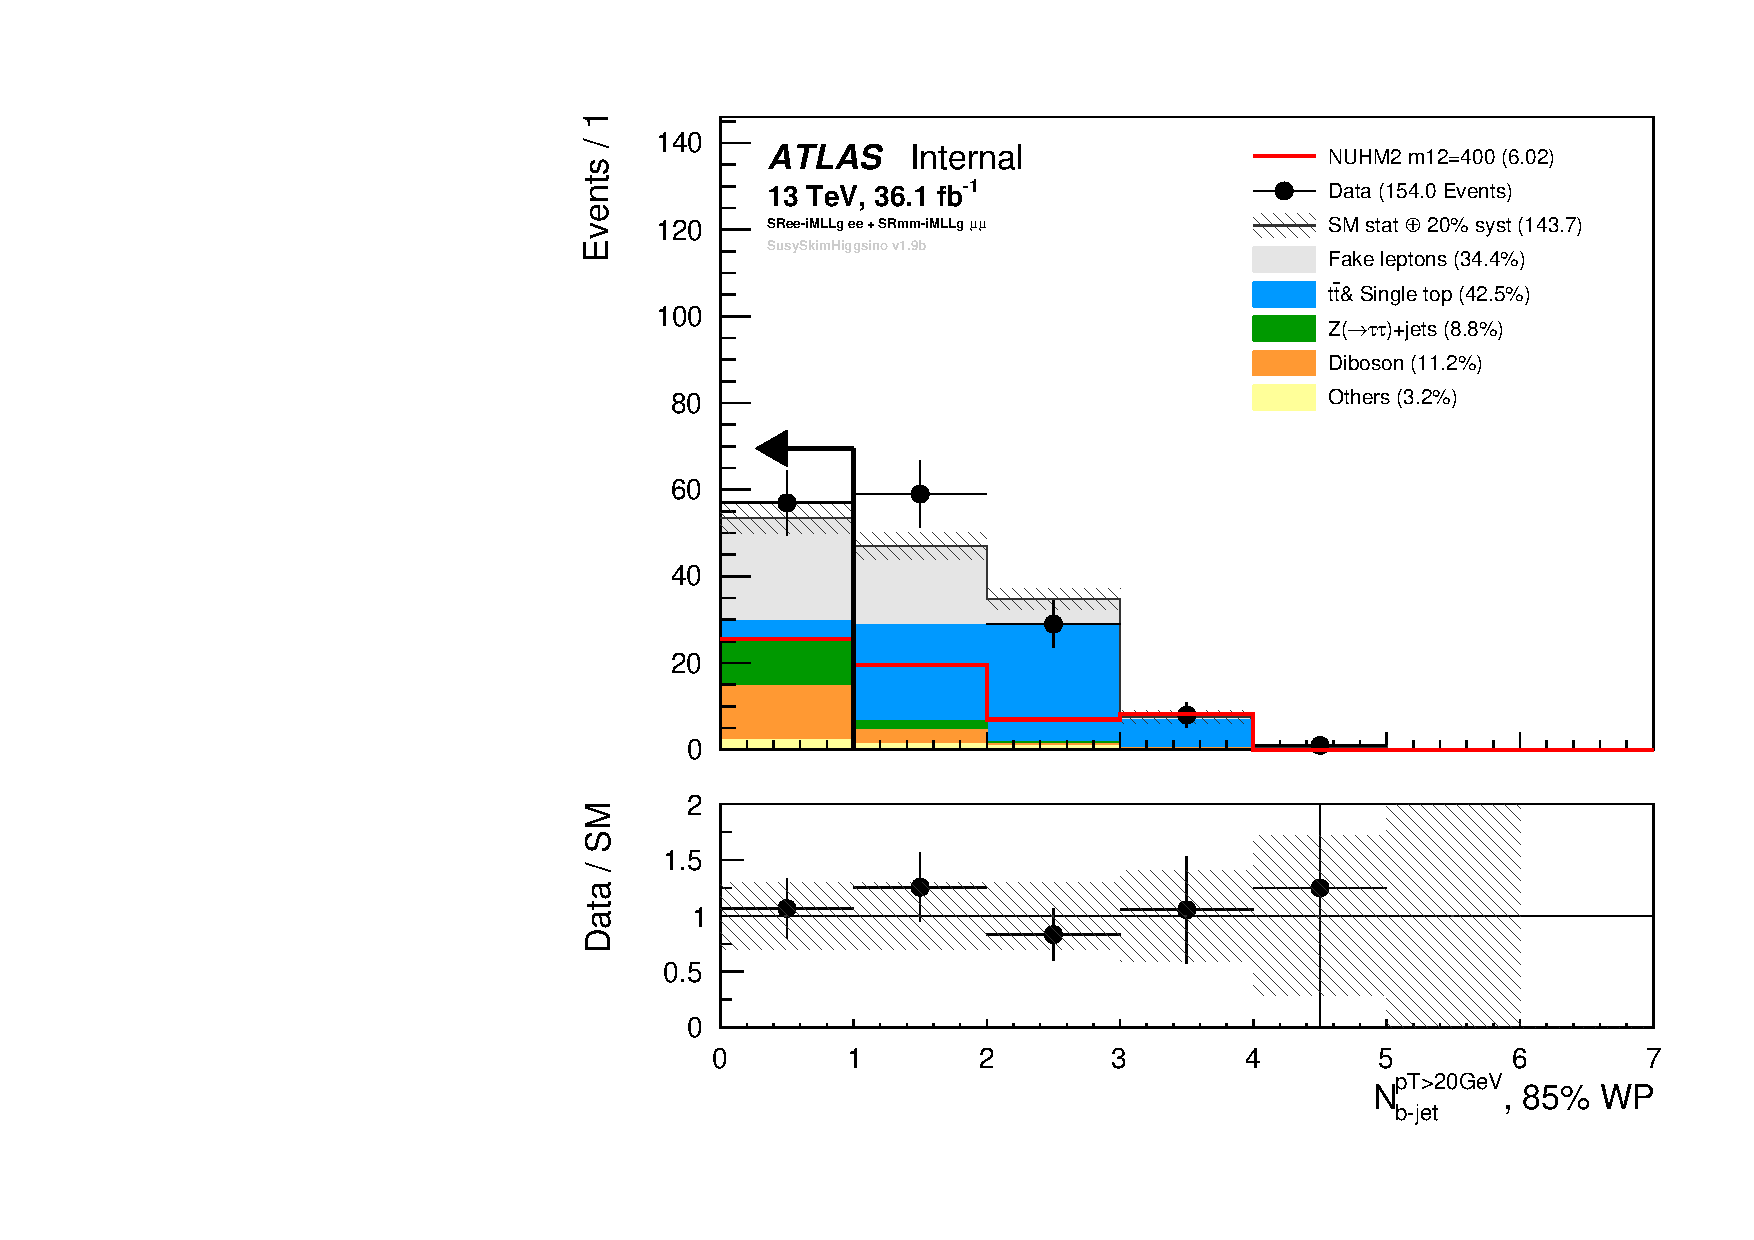
\includegraphics[scale=0.3]{NUHM2_m12_400_and_Bkg_nBJet20_MV2c10_SFOS_N_minus_one_distribution_in_SR_times_10_on_Nsig.pdf}
            \caption{$N^{20}_{\mathrm{b-jets}}$}
            \label{fig:event_nuhm2_m12_400_nBJet20_SFOS}
        \end{subfigure}
        \begin{subfigure}[b]{0.48\textwidth}
            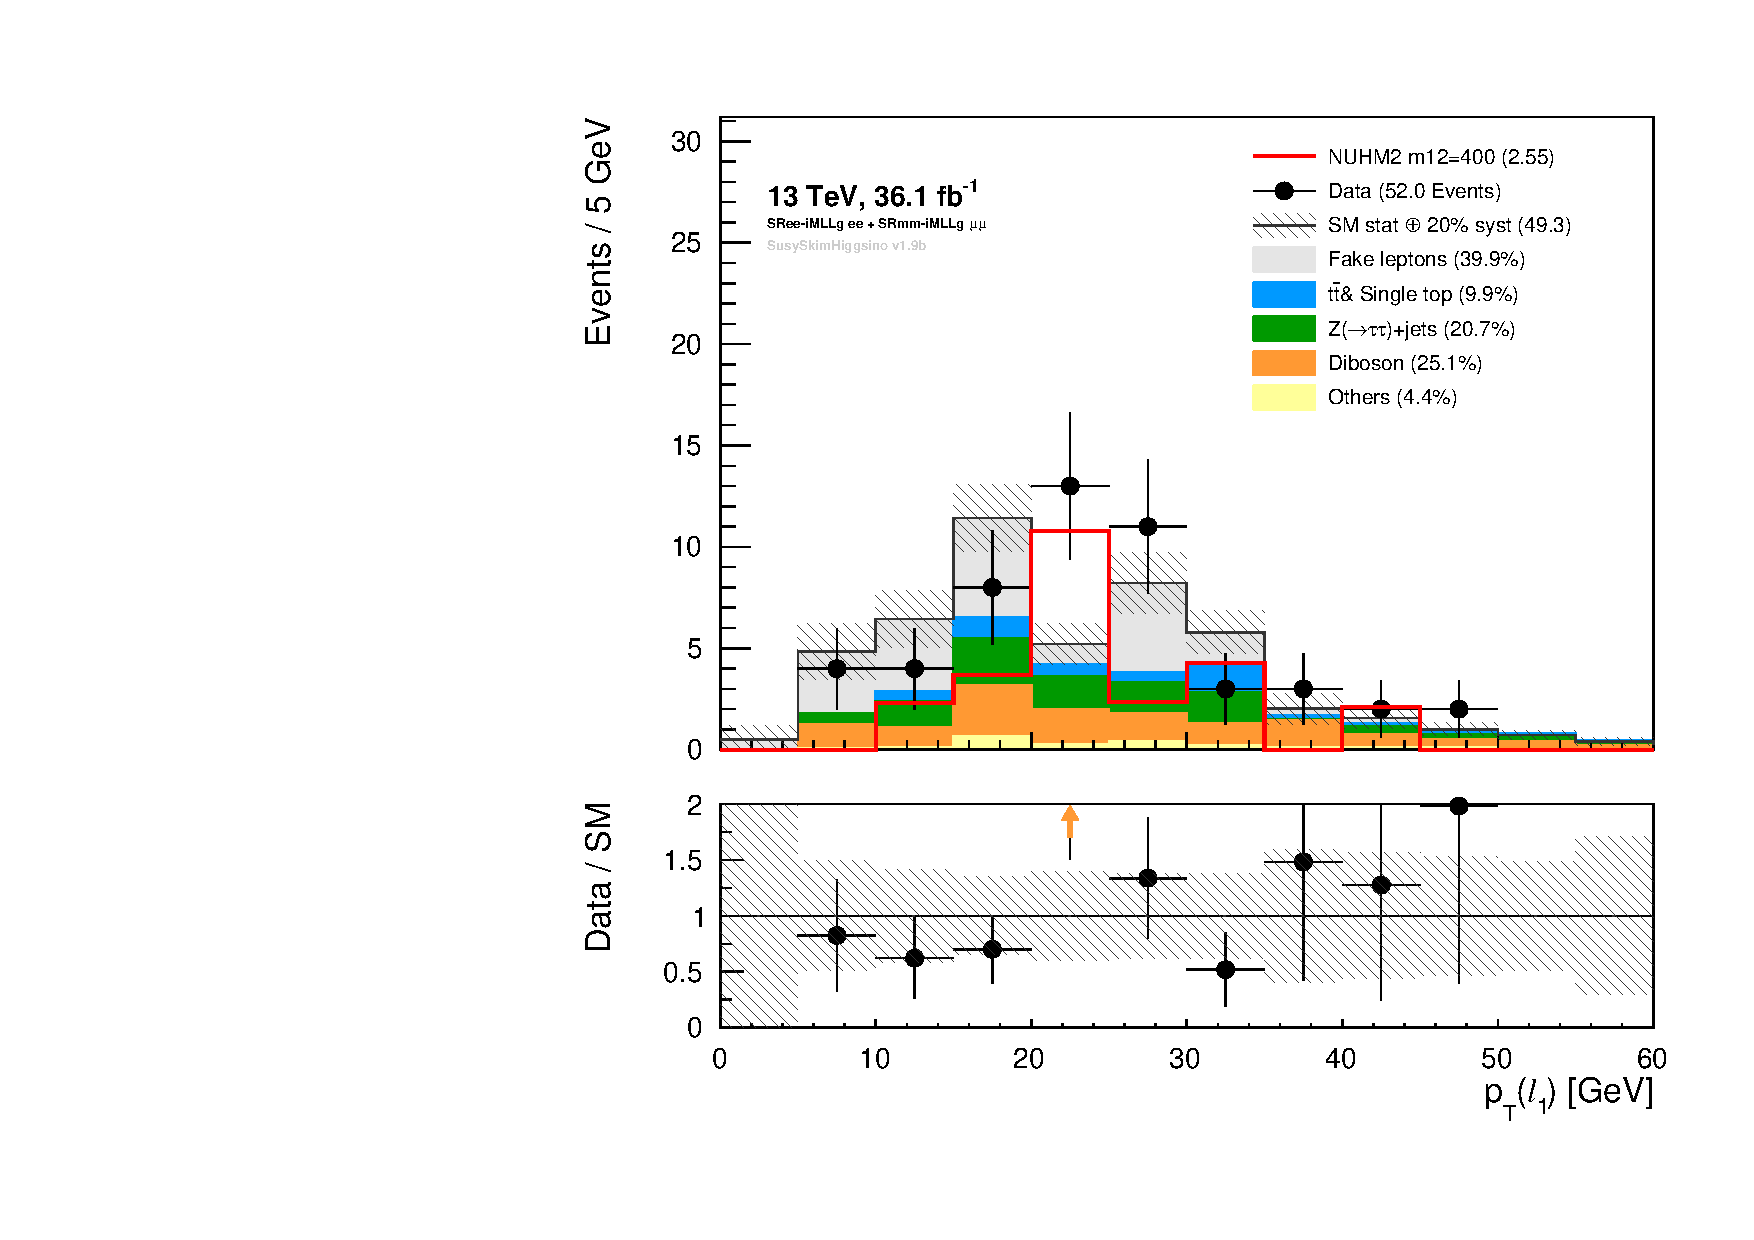
\includegraphics[scale=0.3]{NUHM2_m12_400_and_Bkg_lep1Pt_SFOS_N_minus_one_distribution_in_SR_times_10_on_Nsig.pdf}
            \caption{$p^{\ell_1}_{\mathrm{T}}$}
            \label{fig:event_nuhm2_m12_400_lep1Pt_SFOS}
        \end{subfigure}
        \begin{subfigure}[b]{0.48\textwidth}
            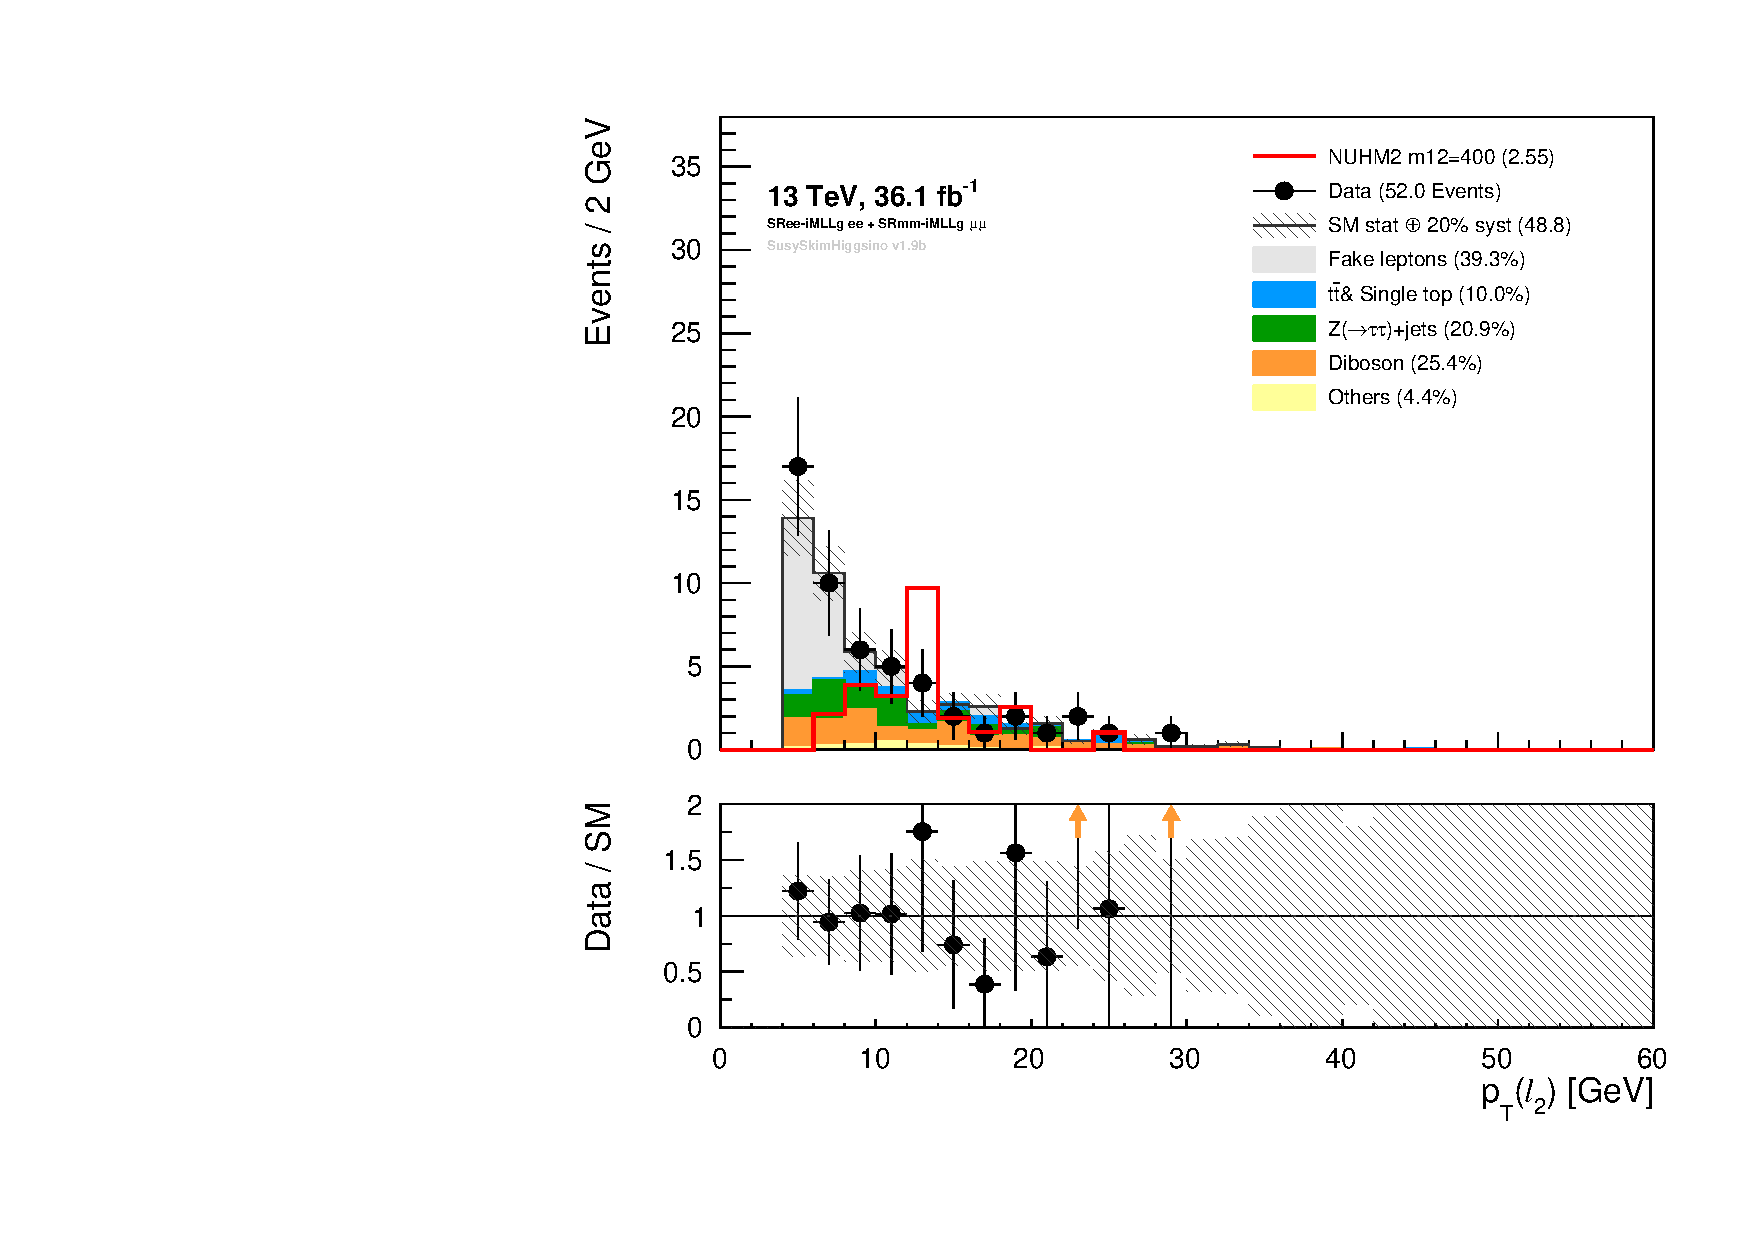
\includegraphics[scale=0.3]{NUHM2_m12_400_and_Bkg_lep2Pt_SFOS_N_minus_one_distribution_in_SR_times_10_on_Nsig.pdf}
            \caption{$p^{\ell_2}_{\mathrm{T}}$}
            \label{fig:event_nuhm2_m12_400_lep2Pt_SFOS}
        \end{subfigure}
        \begin{subfigure}[b]{0.48\textwidth}
            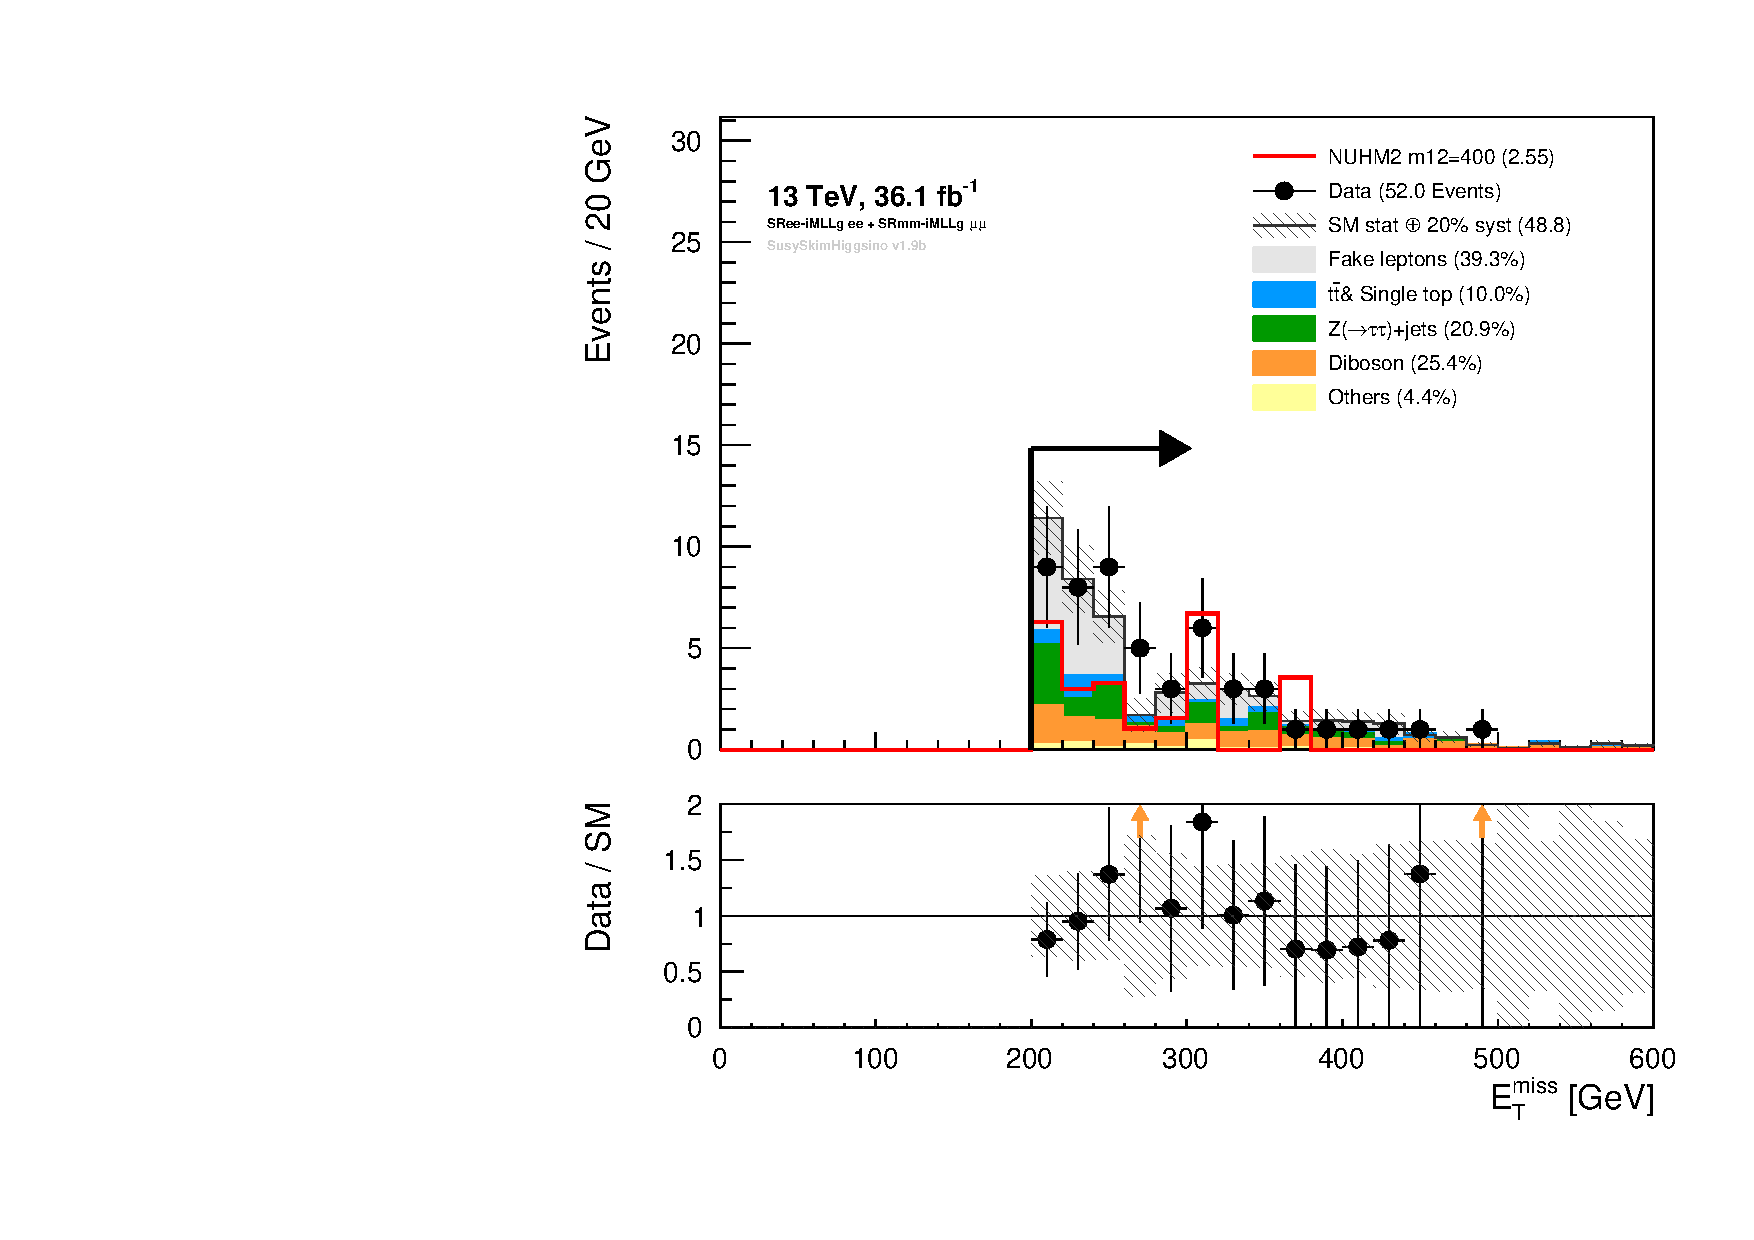
\includegraphics[scale=0.3]{NUHM2_m12_400_and_Bkg_met_Et_SFOS_N_minus_one_distribution_in_SR_times_10_on_Nsig.pdf}
            \caption{$E^{\mathrm{miss}}_{\mathrm{T}}$}
            \label{fig:event_nuhm2_m12_400_met_SFOS}
        \end{subfigure}
        \begin{subfigure}[b]{0.48\textwidth}
            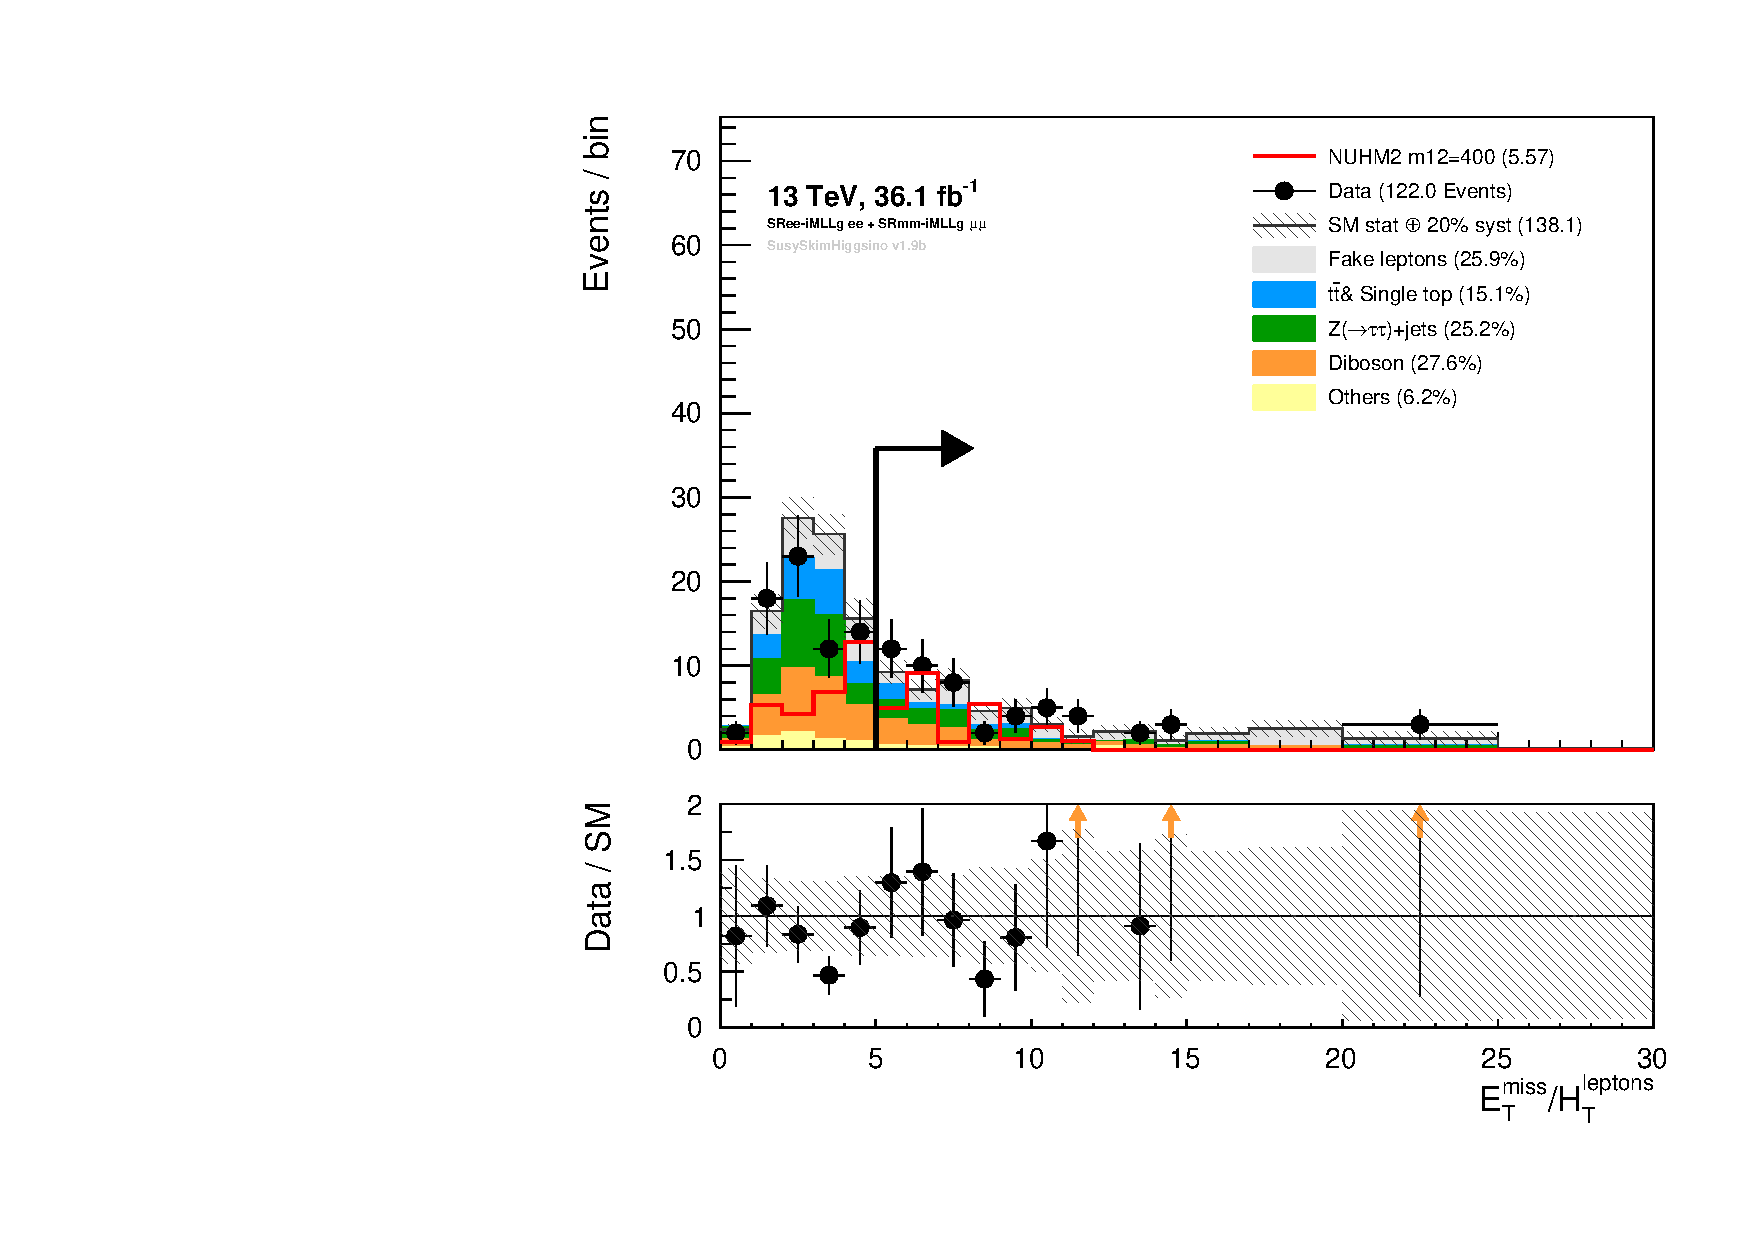
\includegraphics[scale=0.3]{NUHM2_m12_400_and_Bkg_METOverHTLep_SFOS_N_minus_one_distribution_in_SR_times_10_on_Nsig.pdf}
            \caption{$E^{\mathrm{miss}}_{\mathrm{T}} / H^{\mathrm{leptons}}_{\mathrm{T}}$}
            \label{fig:event_nuhm2_m12_400_METOverHTLep_SFOS}
        \end{subfigure}
    \end{center}
    \caption{The `$N-1$' distributions for NUHM2 model with $m_{1/2} = 400$~{\GeV} in SR region $1 < $SR$\ell \ell$-$m_{\ell \ell} < 60$~{\GeV}.
    The NUHM2 distributions are multiplied by 10 but the number of events in the legend use its actual values.}
    \label{fig:dist_nuhm2_kinematic_in_SR_SFOS_m12_400_1}
\end{figure}

\begin{figure}[htbp]
    \begin{center}
        \begin{subfigure}[b]{0.48\textwidth}
            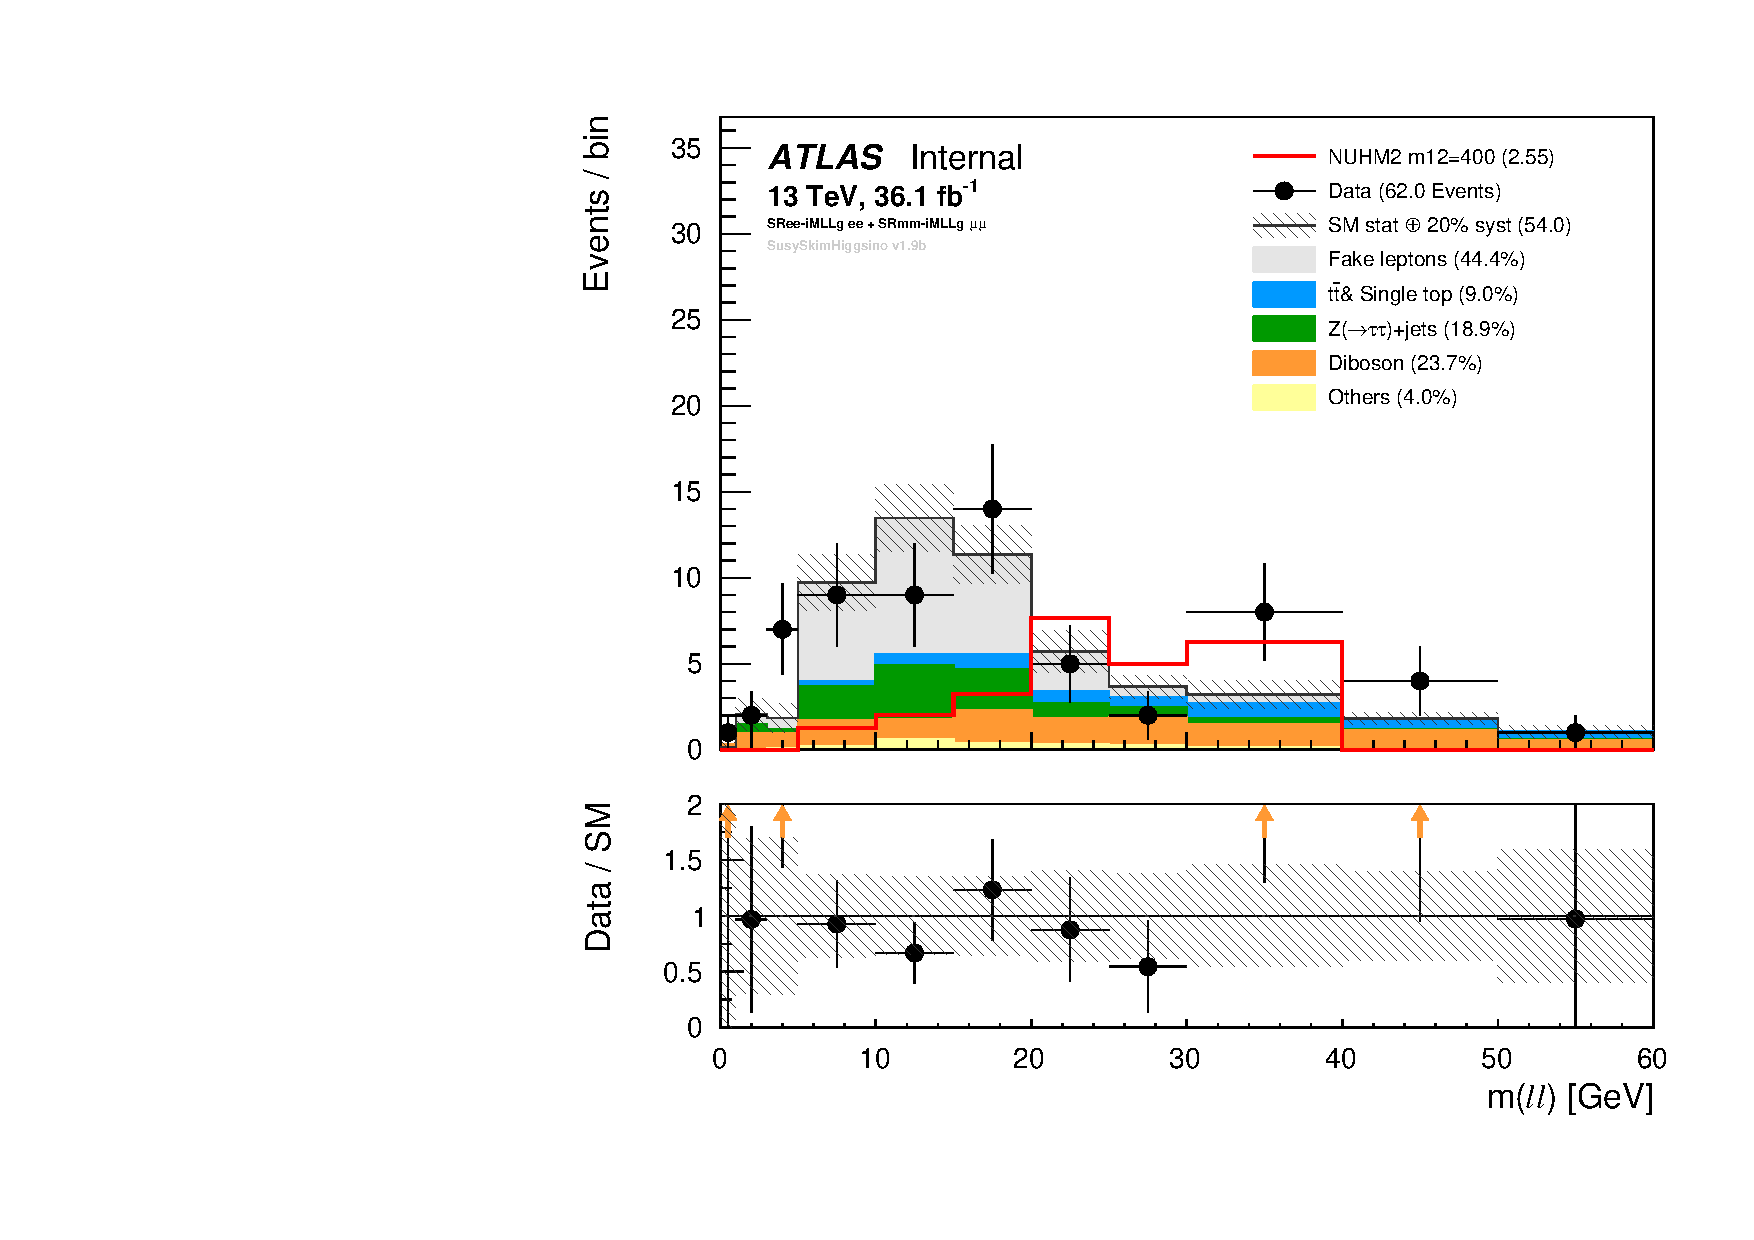
\includegraphics[scale=0.3]{NUHM2_m12_400_and_Bkg_mll_SFOS_N_minus_one_distribution_in_SR_times_10_on_Nsig.pdf}
            \caption{$m_{\ell\ell}$}
            \label{fig:event_nuhm2_m12_400_mll_SFOS}
        \end{subfigure}
        \begin{subfigure}[b]{0.48\textwidth}
            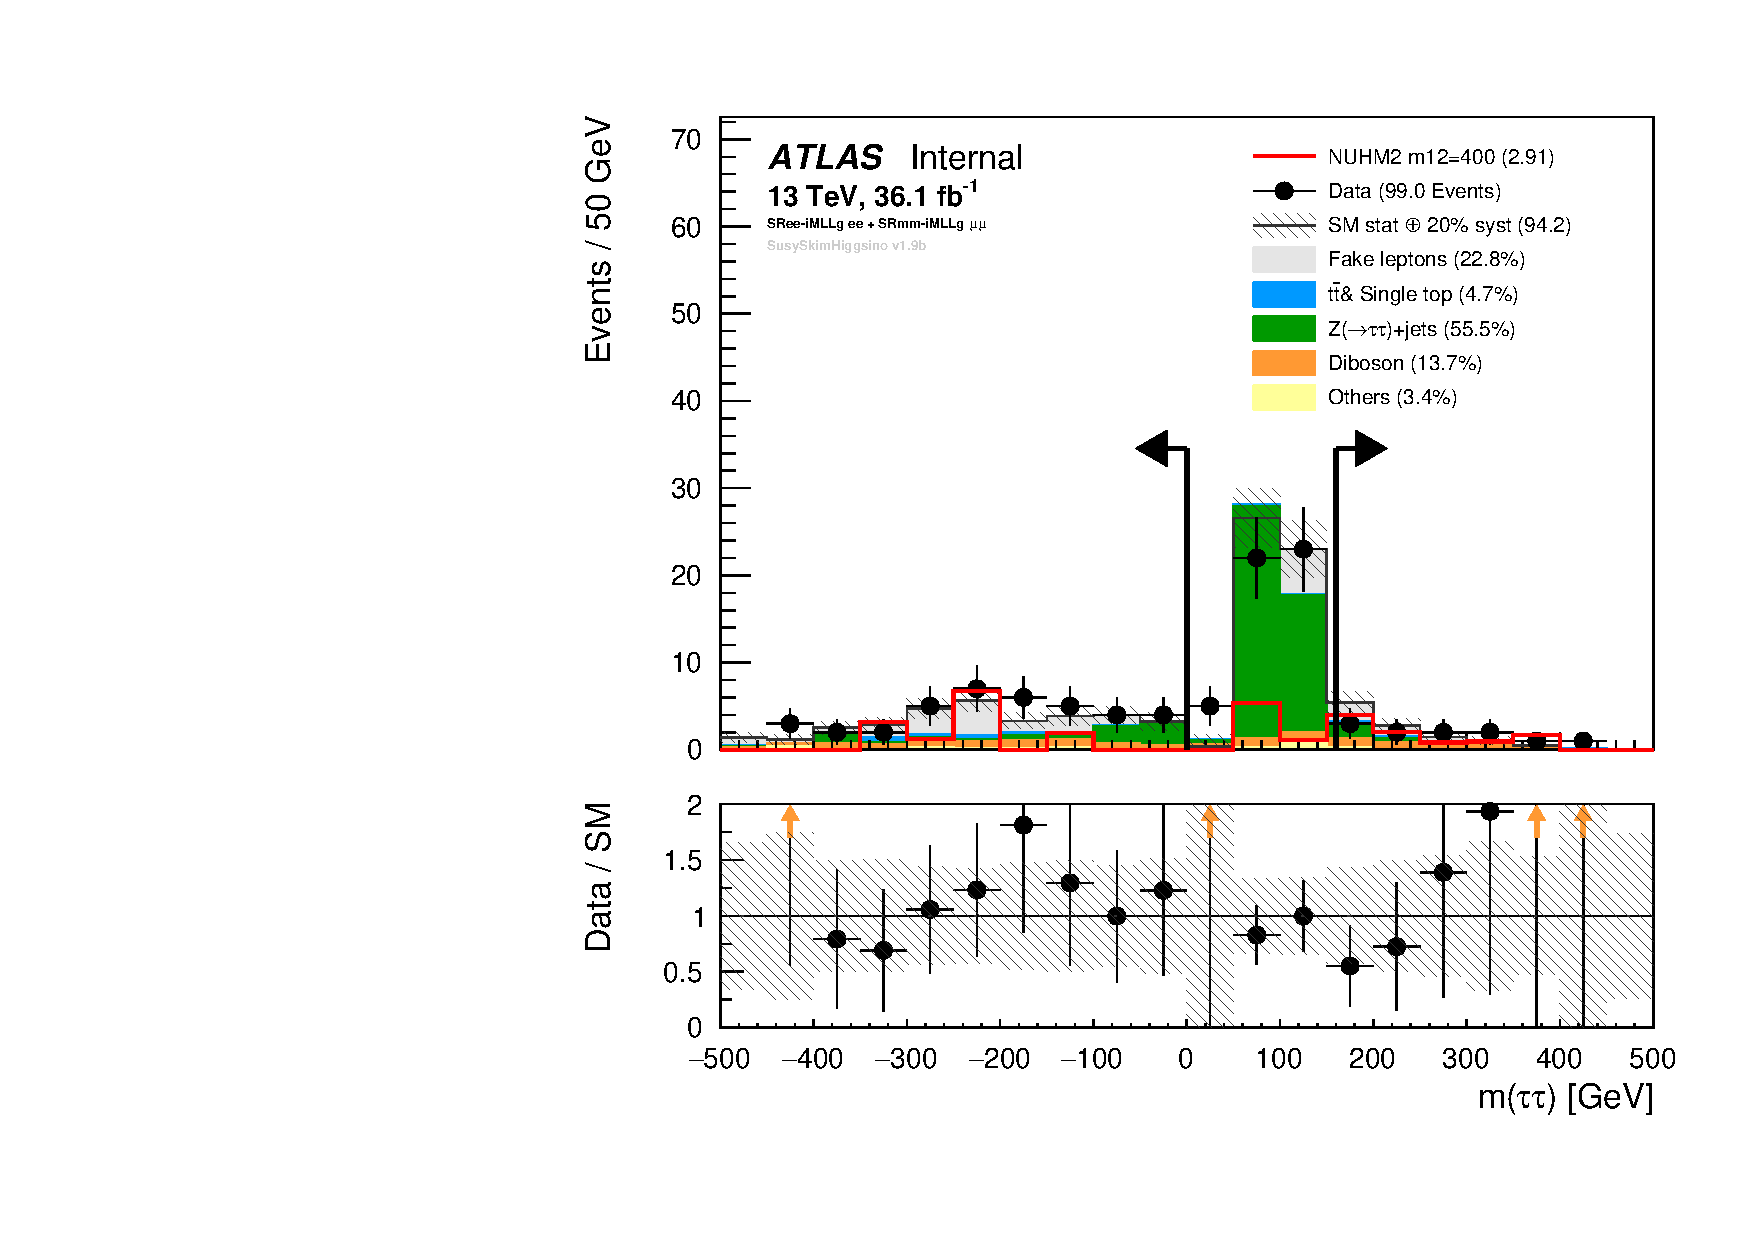
\includegraphics[scale=0.3]{NUHM2_m12_400_and_Bkg_MTauTau_SFOS_N_minus_one_distribution_in_SR_times_10_on_Nsig.pdf}
            \caption{$m_{\tau\tau}$}
            \label{fig:event_nuhm2_m12_400_MTauTau_SFOS}
        \end{subfigure}
        \begin{subfigure}[b]{0.48\textwidth}
            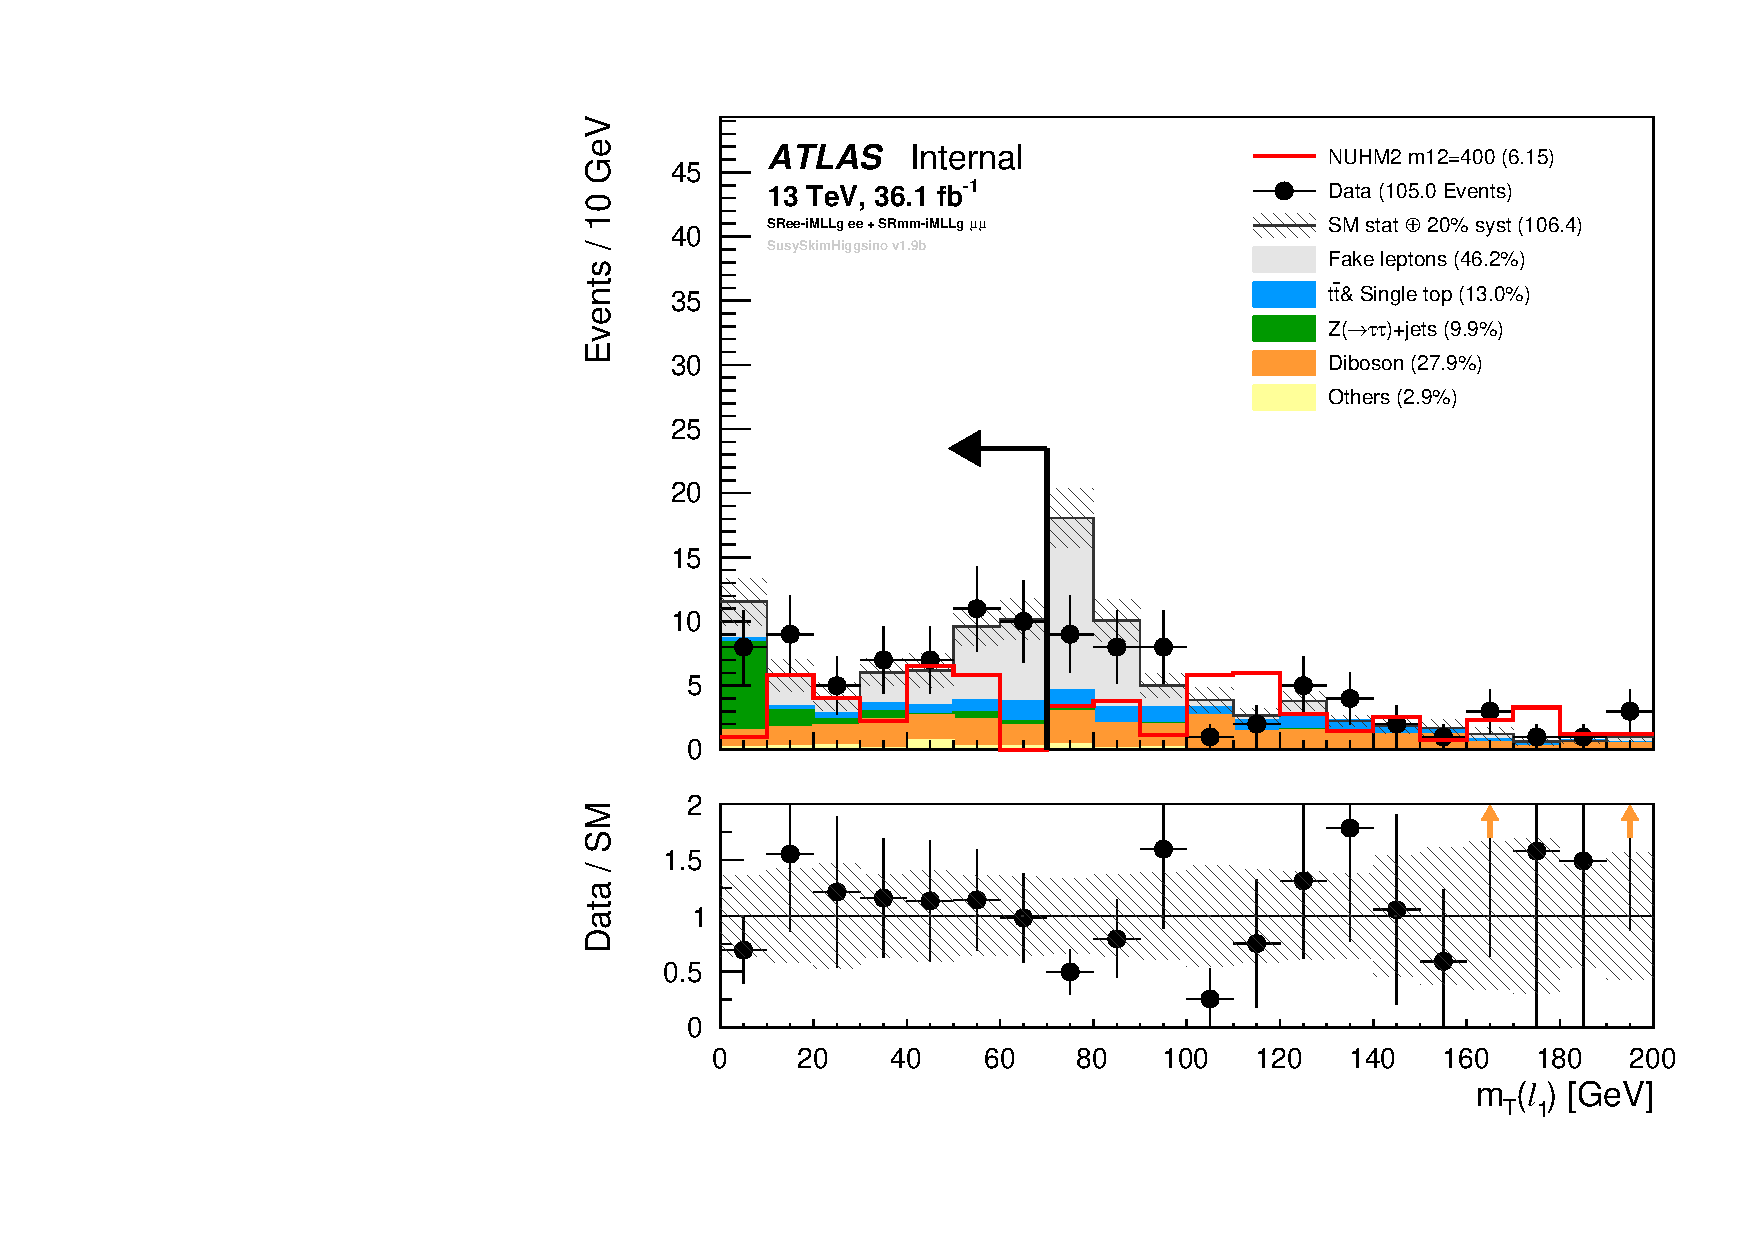
\includegraphics[scale=0.3]{NUHM2_m12_400_and_Bkg_mt_lep1_SFOS_N_minus_one_distribution_in_SR_times_10_on_Nsig.pdf}
            \caption{$m_{T}(\ell_{1})$}
            \label{fig:event_nuhm2_m12_400_mt_lep1_SFOS}
        \end{subfigure}
        \begin{subfigure}[b]{0.48\textwidth}
            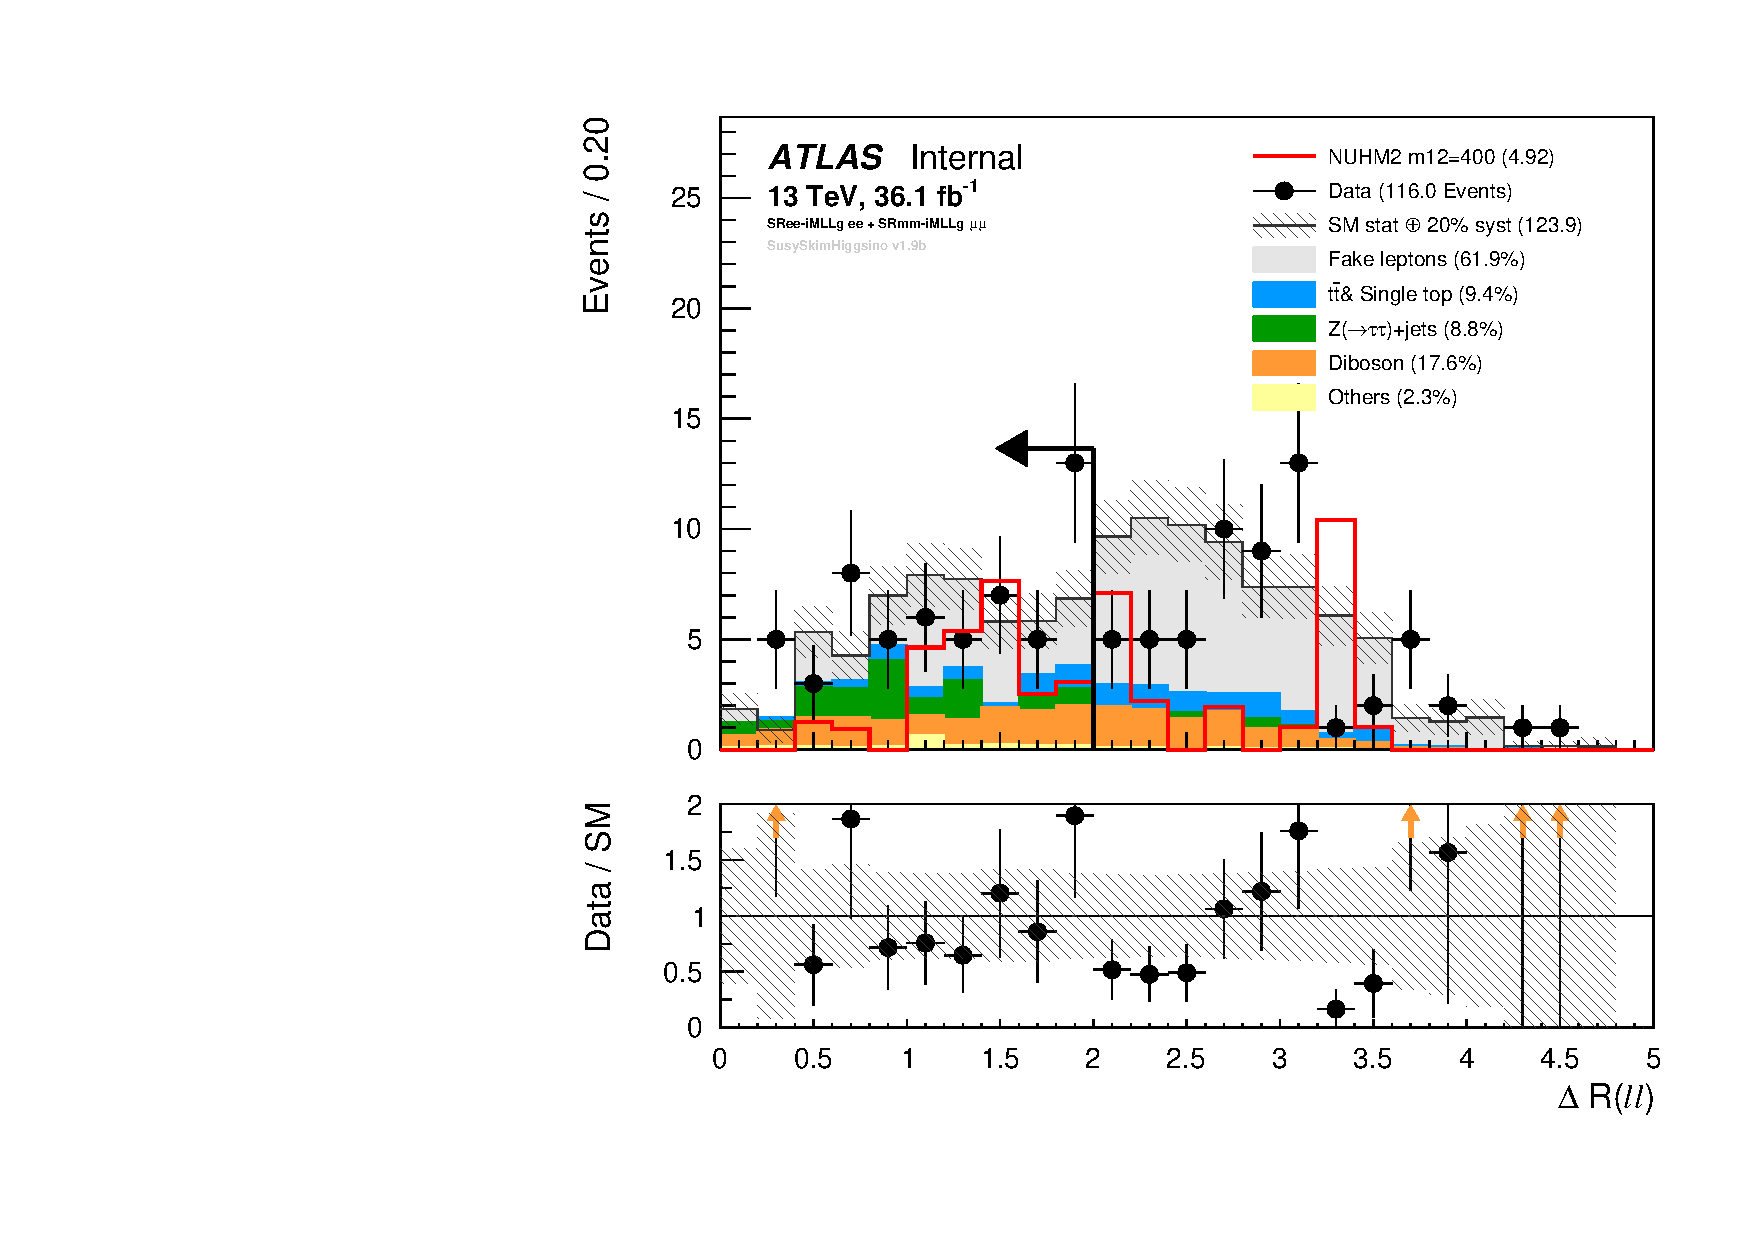
\includegraphics[scale=0.3]{NUHM2_m12_400_and_Bkg_Rll_SFOS_N_minus_one_distribution_in_SR_times_10_on_Nsig.pdf}
            \caption{$\Delta R_{\ell\ell}$}
            \label{fig:event_nuhm2_m12_400_Rll_SFOS}
        \end{subfigure}
        \begin{subfigure}[b]{0.48\textwidth}
            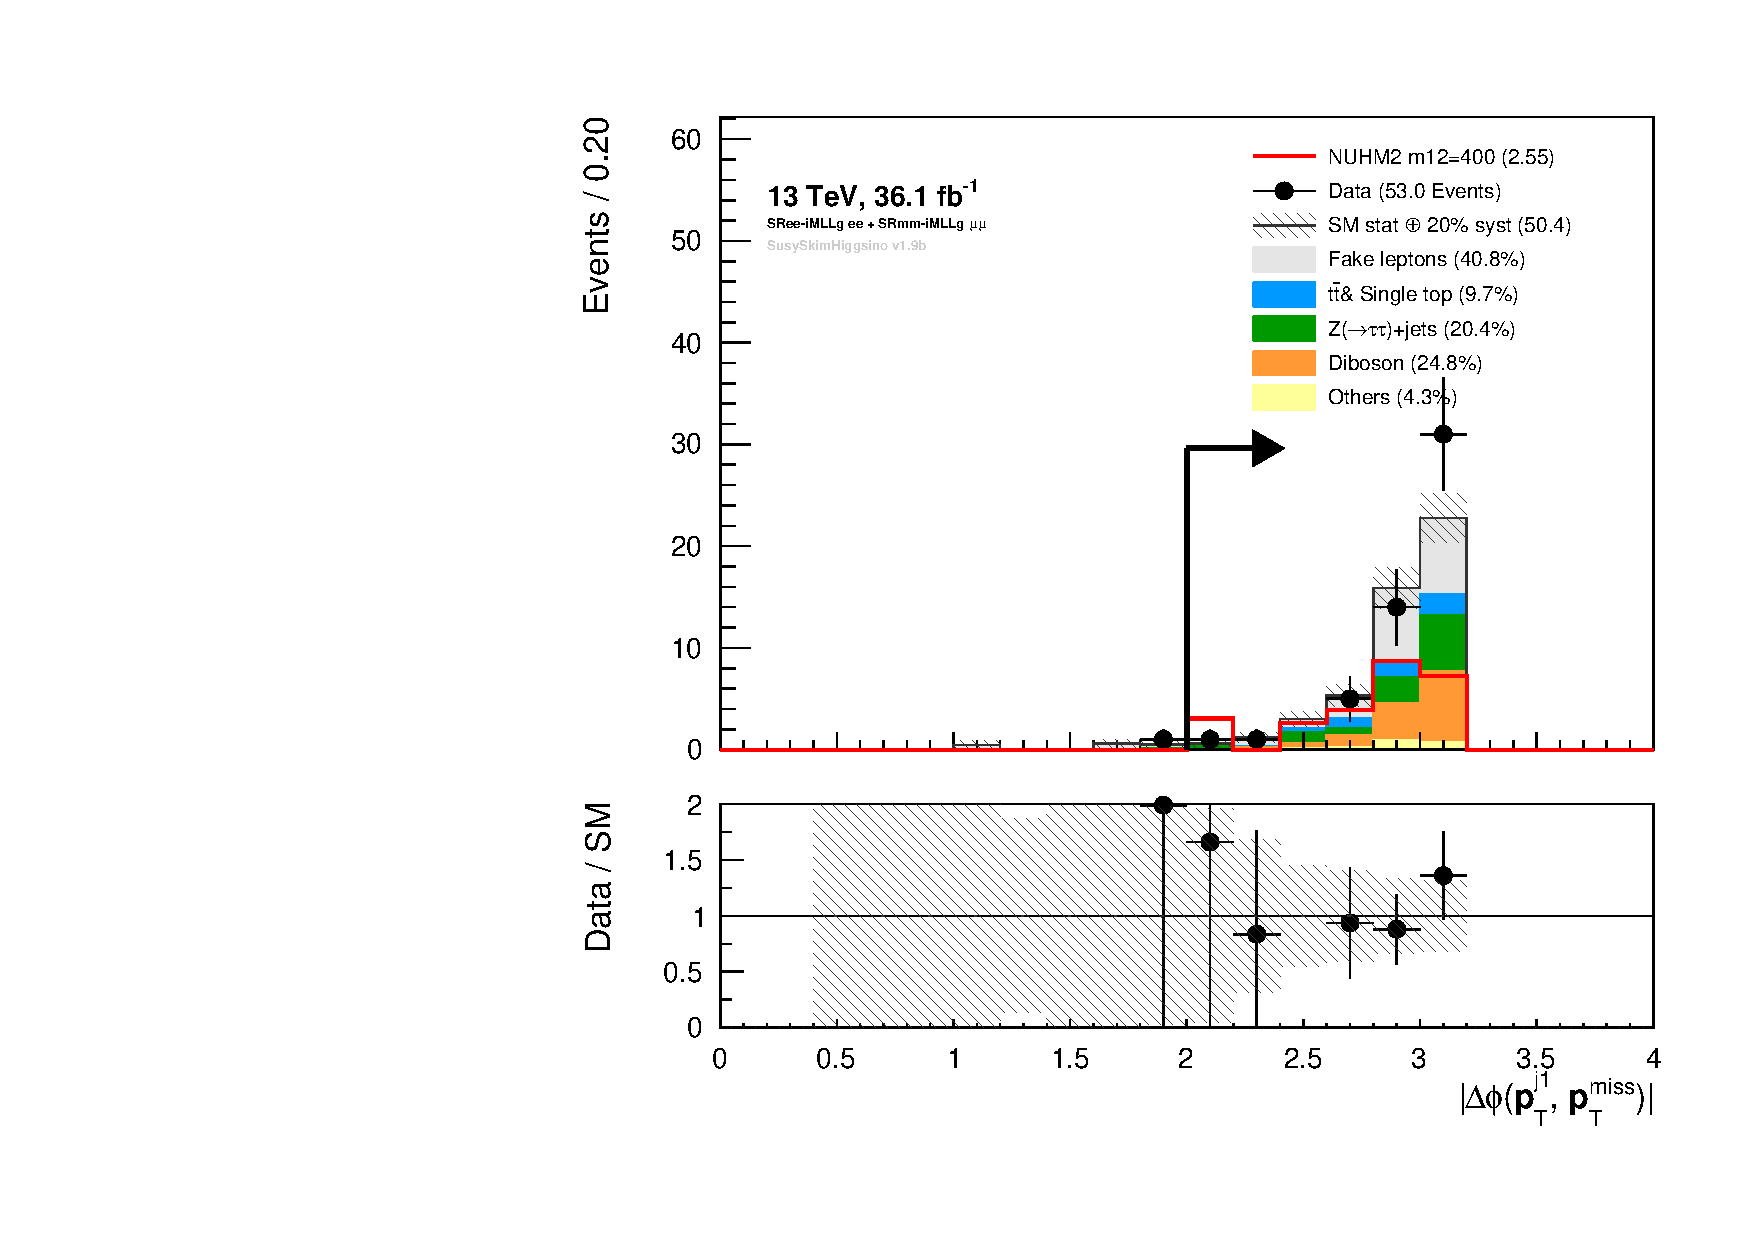
\includegraphics[scale=0.3]{NUHM2_m12_400_and_Bkg_DPhiJ1Met_SFOS_N_minus_one_distribution_in_SR_times_10_on_Nsig.pdf}
            \caption{$|\Delta \phi(\mathbf{p}^{j_{1}}_{\mathrm{T}}, \mathbf{p}^{\mathrm{miss}}_{\mathrm{T}})|$}
            \label{fig:event_nuhm2_m12_400_DPhiJ1Met_SFOS}
        \end{subfigure}
        \begin{subfigure}[b]{0.48\textwidth}
            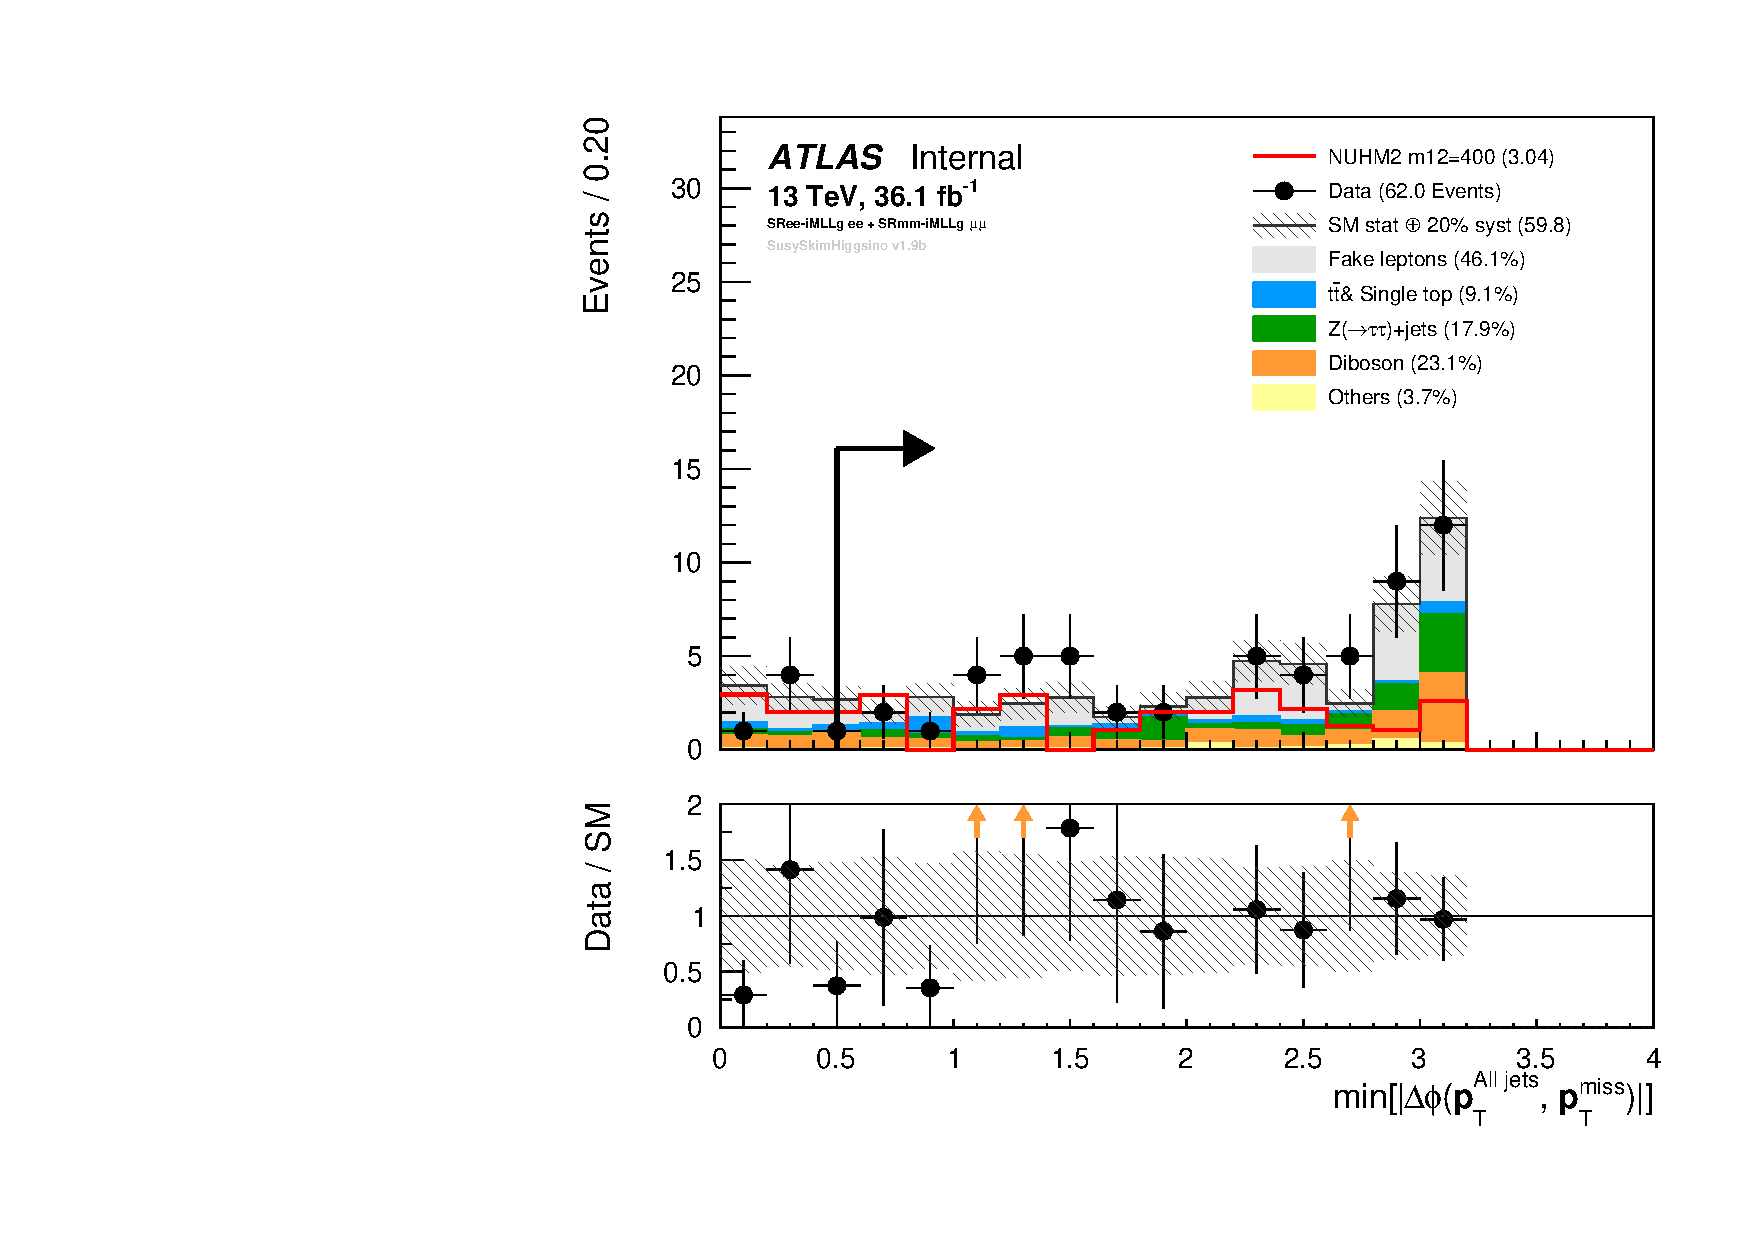
\includegraphics[scale=0.3]{NUHM2_m12_400_and_Bkg_minDPhiAllJetsMet_SFOS_N_minus_one_distribution_in_SR_times_10_on_Nsig.pdf}
            \caption{min[$|\Delta \phi(\mathbf{p}^{\textrm{All jets}}_{\mathrm{T}}, \mathbf{p}^{\mathrm{miss}}_{\mathrm{T}})|$]}
            \label{fig:event_nuhm2_m12_400_minDPhiAllJetsMet_SFOS}
        \end{subfigure}
    \end{center}
    \caption{The `$N-1$' distributions for NUHM2 model with $m_{1/2} = 400$~{\GeV} in SR region $1 < $SR$\ell \ell$-$m_{\ell \ell} < 60$~{\GeV}.
    The NUHM2 distributions are multiplied by 10 but the number of events in the legend use its actual values.}
    \label{fig:dist_nuhm2_kinematic_in_SR_SFOS_m12_400_2}
\end{figure}

% m12 = 500
% \begin{figure}[htbp]
%     \begin{center}
%         \begin{subfigure}[b]{0.48\textwidth}
%             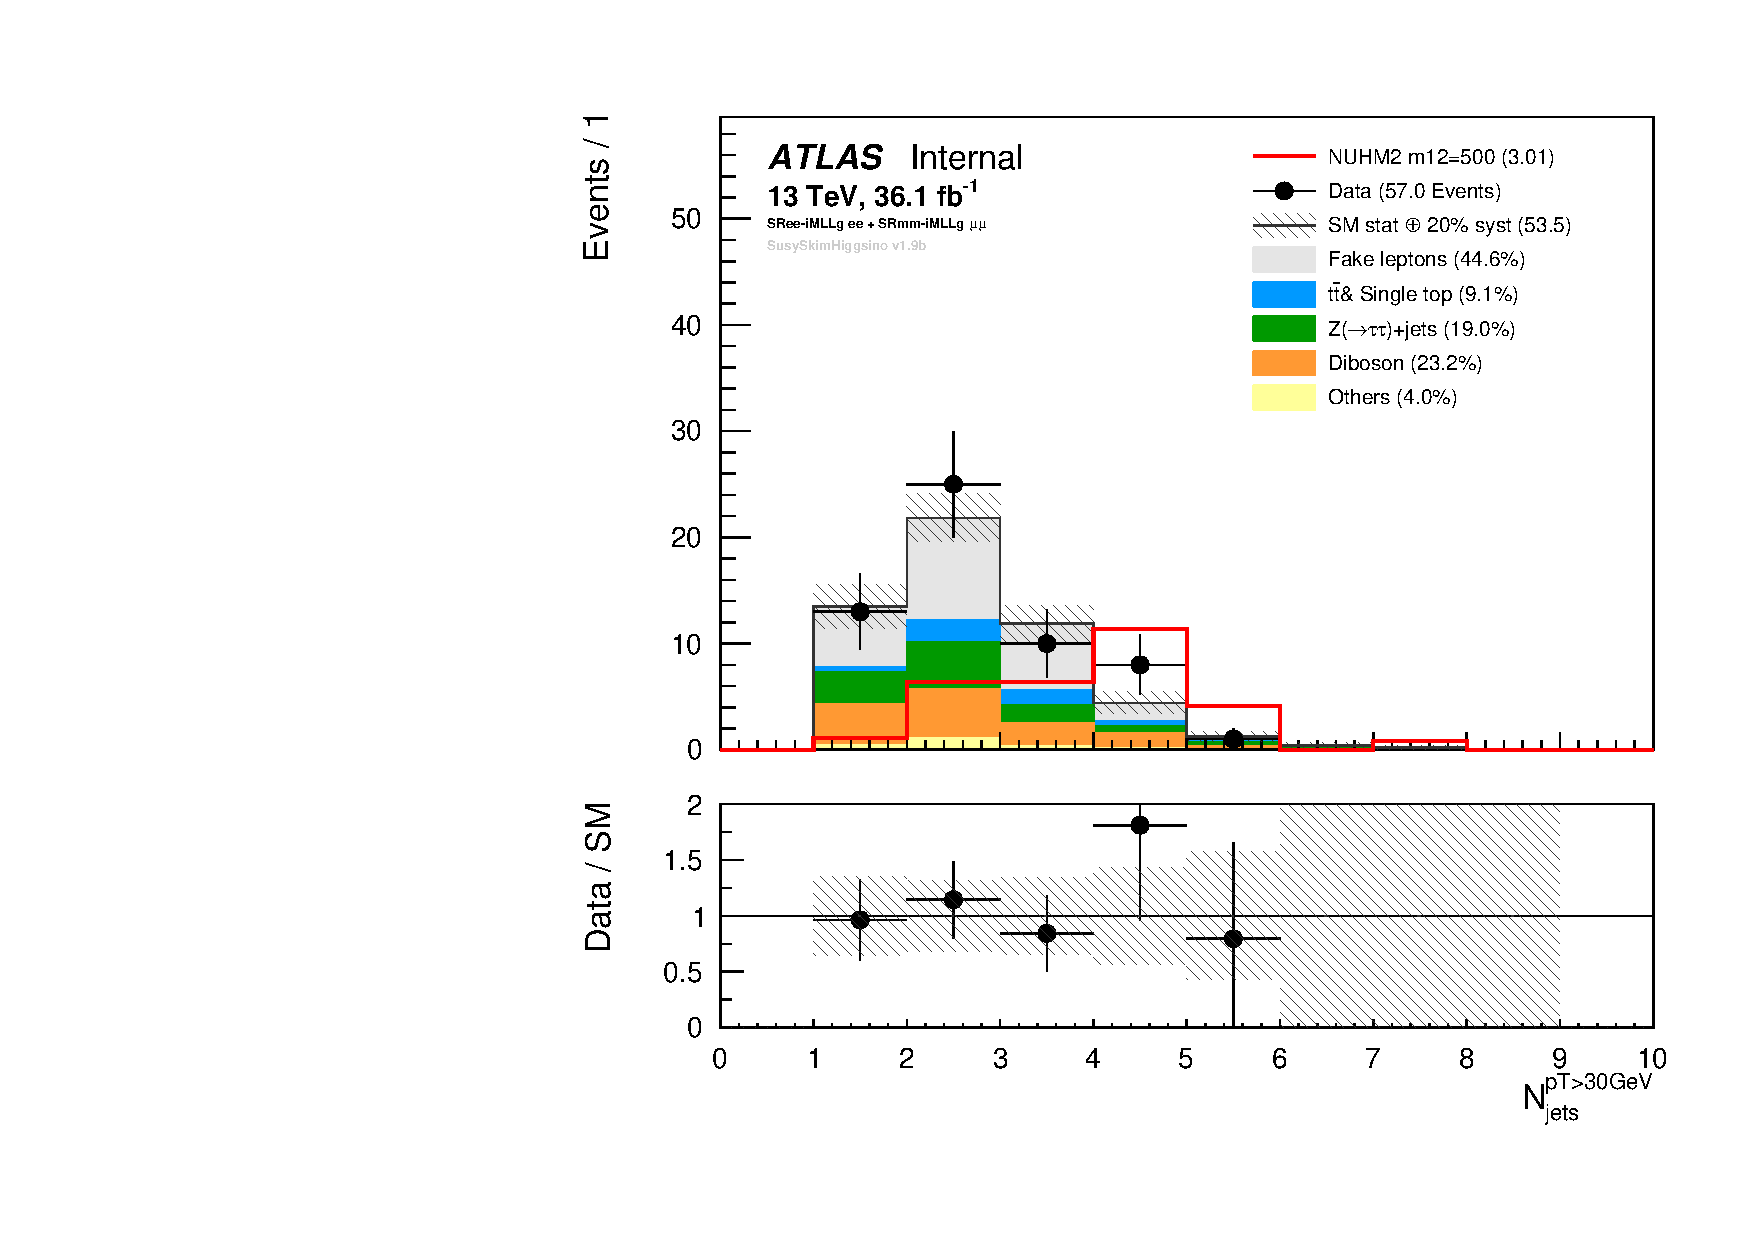
\includegraphics[scale=0.3]{NUHM2_m12_500_and_Bkg_nJet30_SFOS_N_minus_one_distribution_in_SR_times_10_on_Nsig.pdf}
%             \caption{$N^{30}_{\mathrm{jets}}$}
%             \label{fig:event_nuhm2_m12_500_nJet30_SFOS}
%         \end{subfigure}
%         \begin{subfigure}[b]{0.48\textwidth}
%             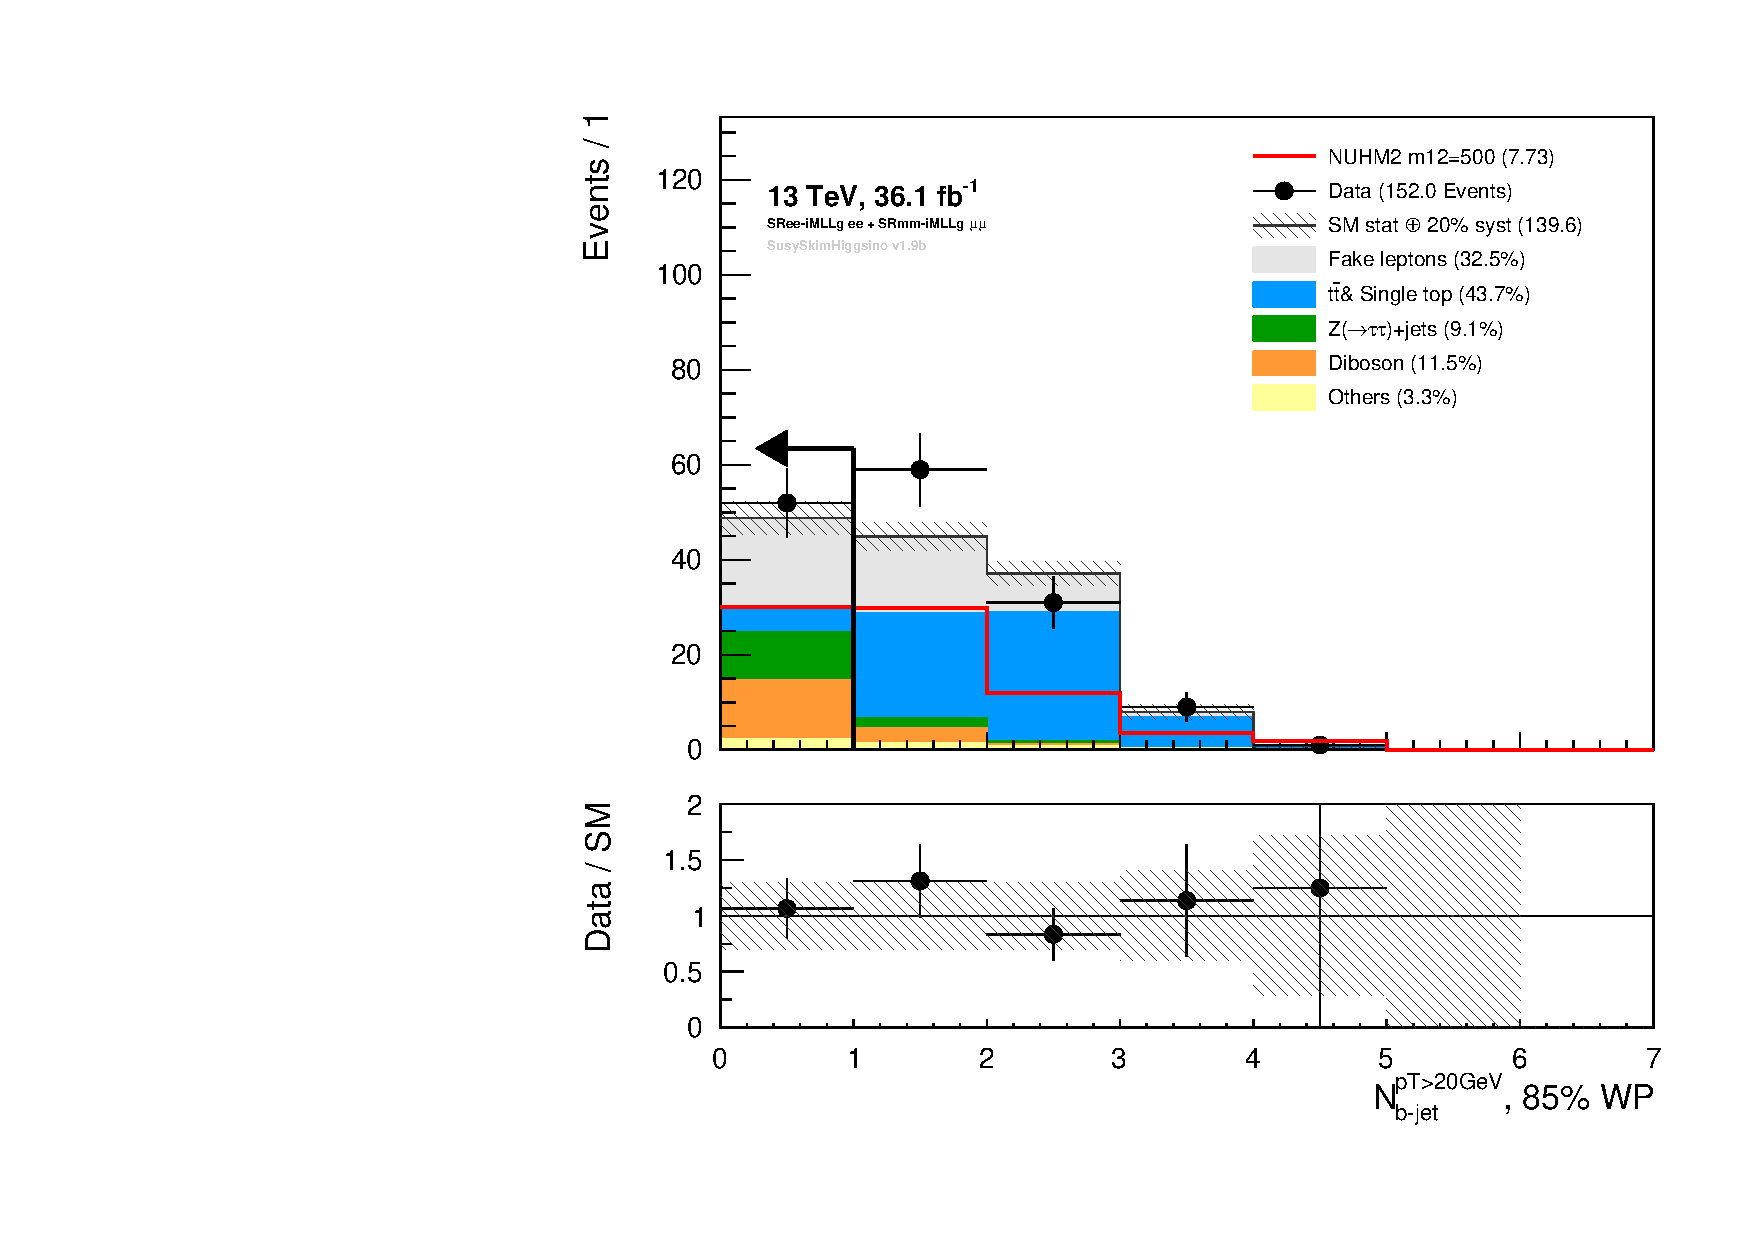
\includegraphics[scale=0.3]{NUHM2_m12_500_and_Bkg_nBJet20_MV2c10_SFOS_N_minus_one_distribution_in_SR_times_10_on_Nsig.pdf}
%             \caption{$N^{20}_{\mathrm{b-jets}}$}
%             \label{fig:event_nuhm2_m12_500_nBJet20_SFOS}
%         \end{subfigure}
%         \begin{subfigure}[b]{0.48\textwidth}
%             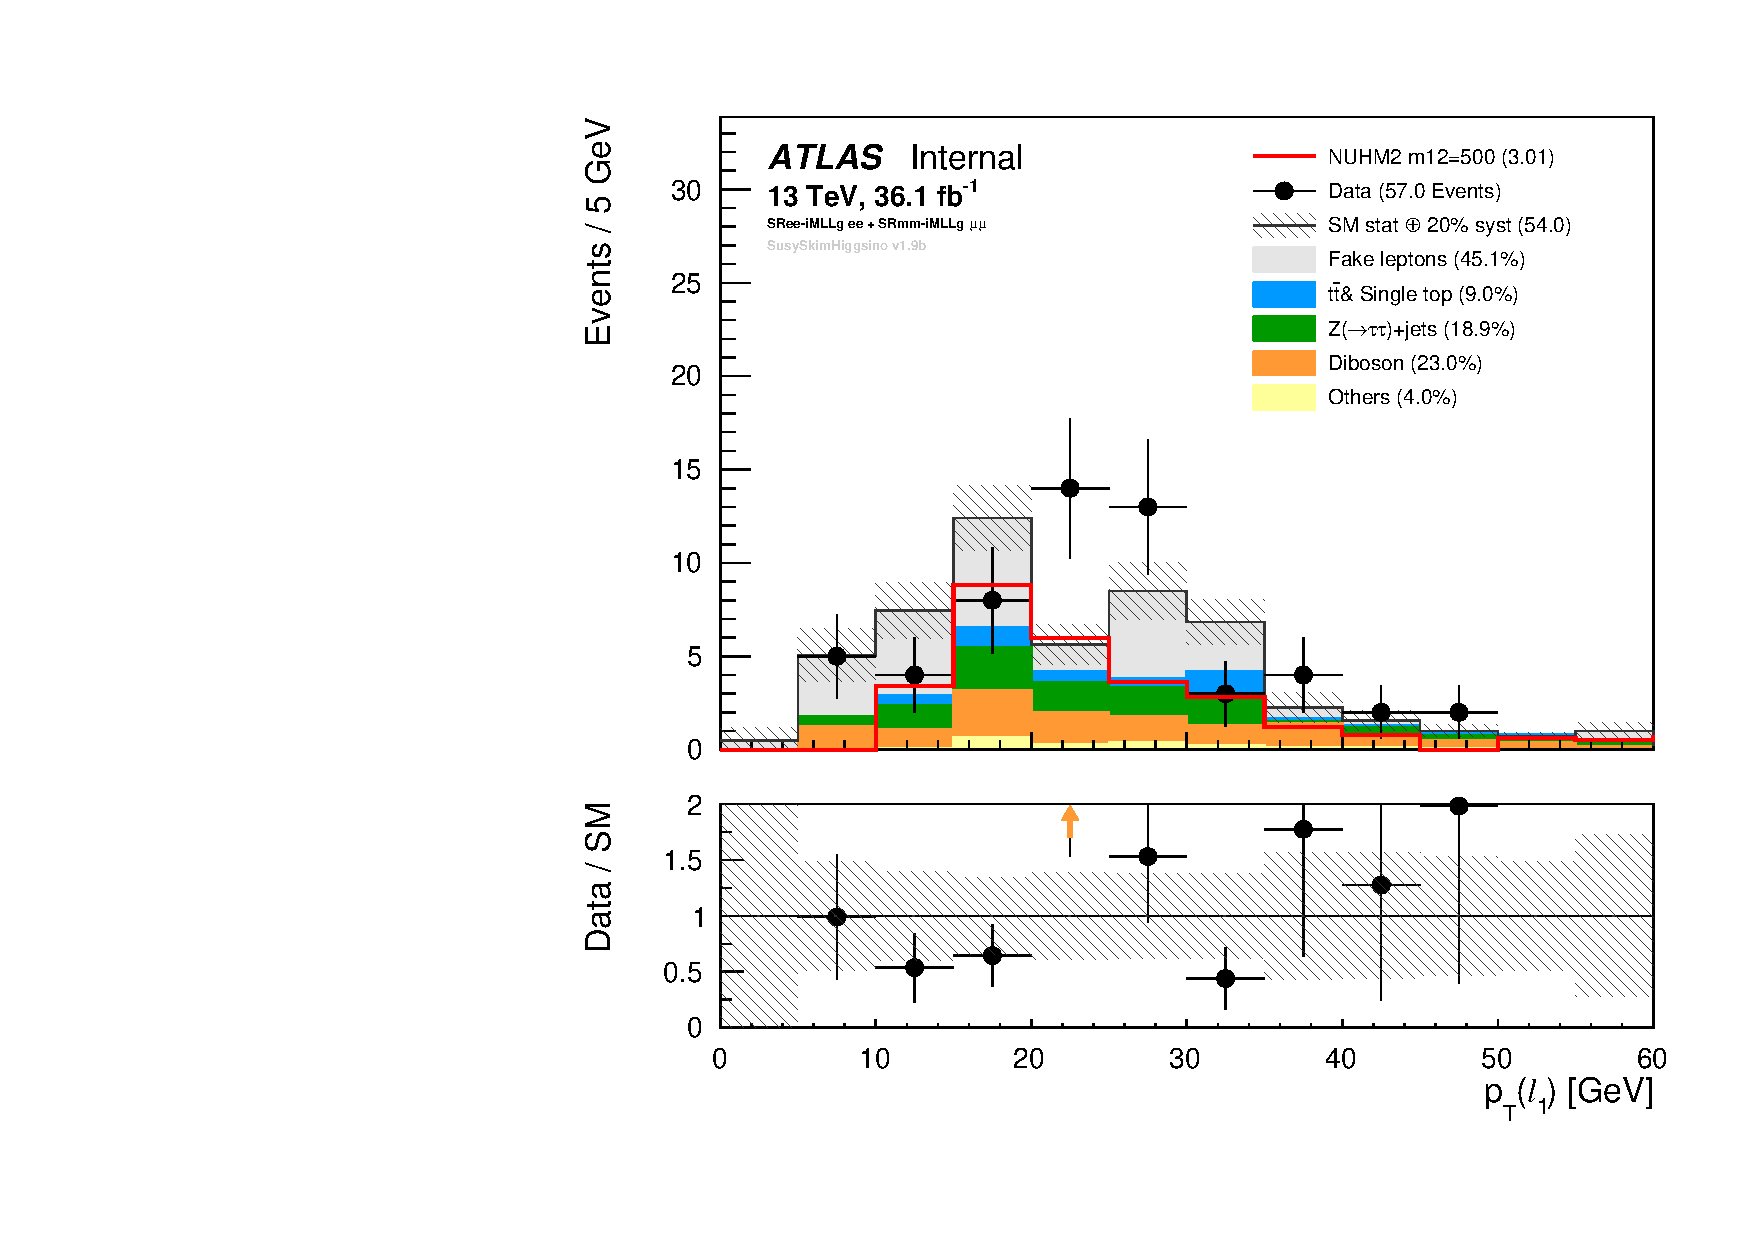
\includegraphics[scale=0.3]{NUHM2_m12_500_and_Bkg_lep1Pt_SFOS_N_minus_one_distribution_in_SR_times_10_on_Nsig.pdf}
%             \caption{$p^{\ell_1}_{\mathrm{T}}$}
%             \label{fig:event_nuhm2_m12_500_lep1Pt_SFOS}
%         \end{subfigure}
%         \begin{subfigure}[b]{0.48\textwidth}
%             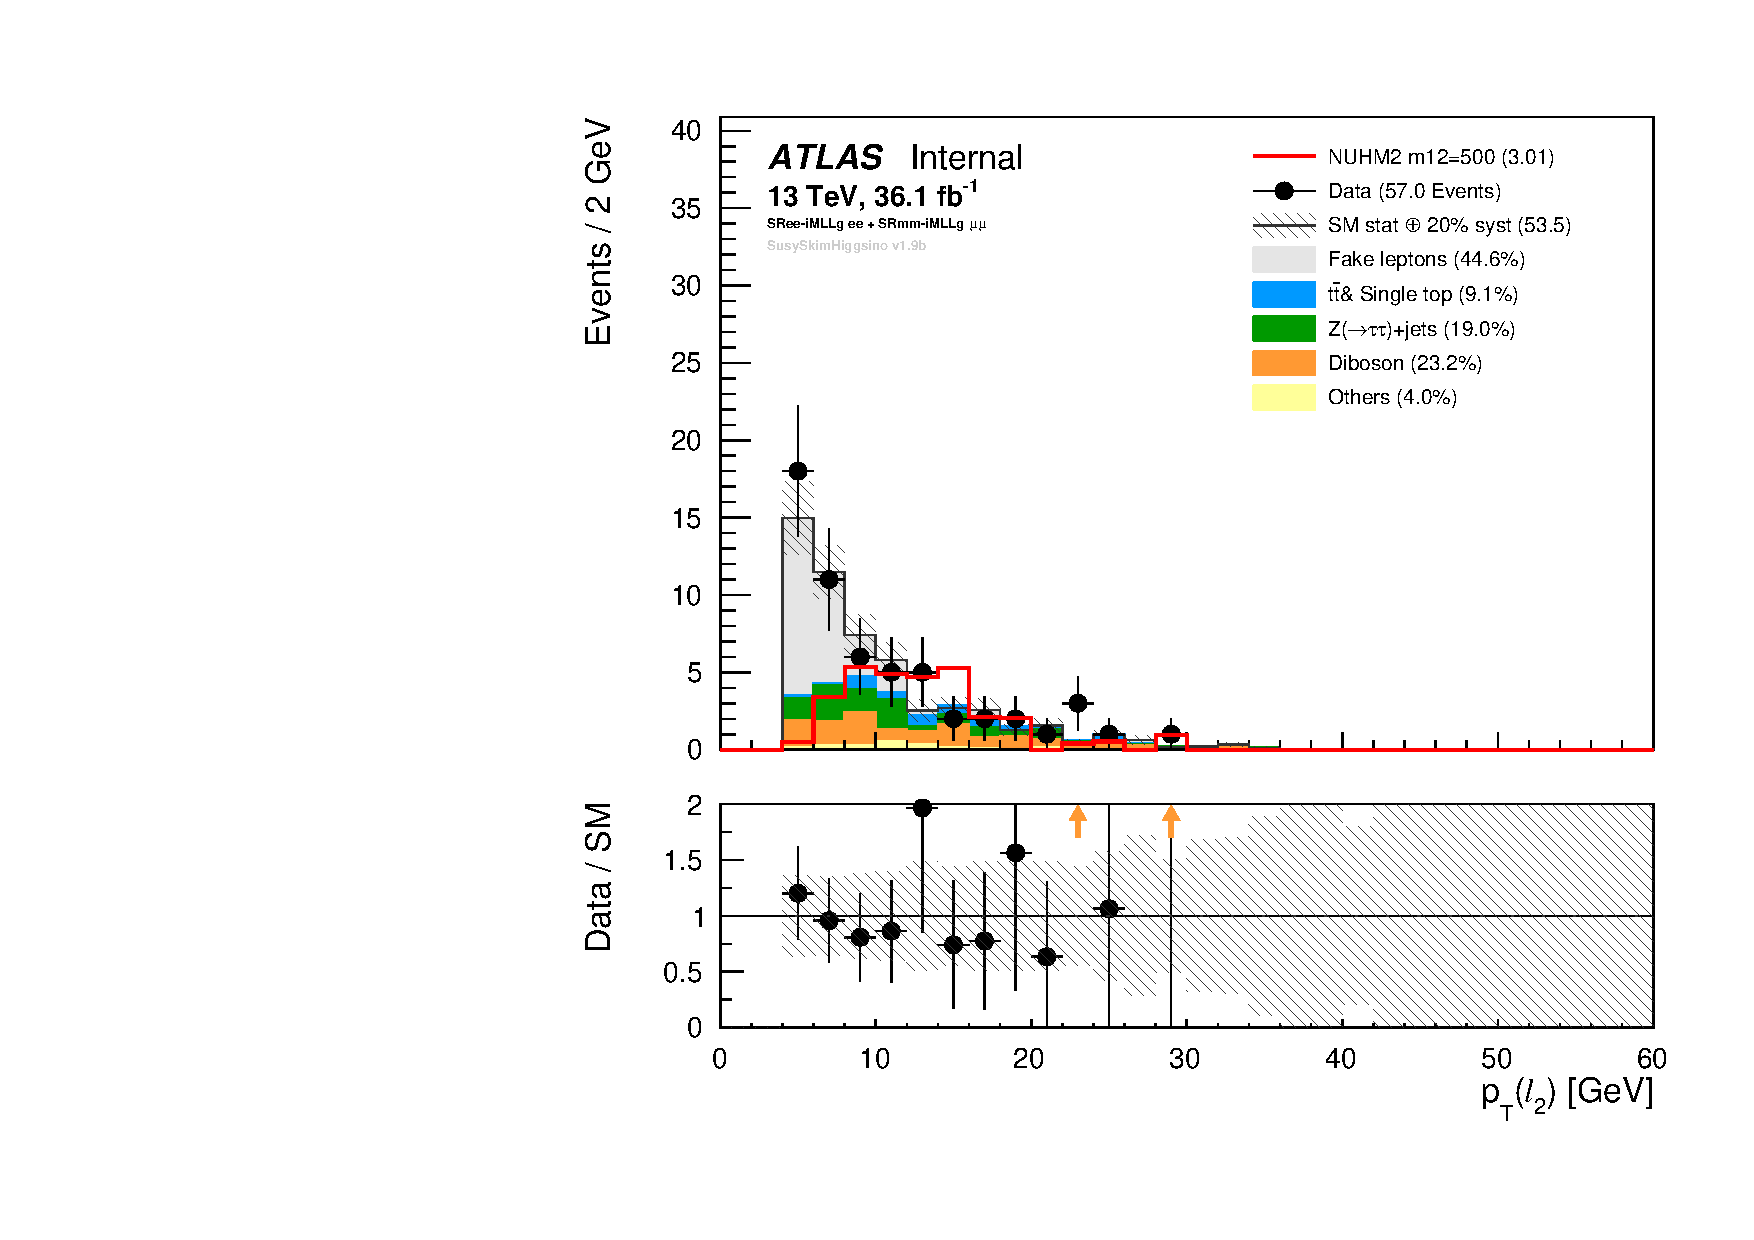
\includegraphics[scale=0.3]{NUHM2_m12_500_and_Bkg_lep2Pt_SFOS_N_minus_one_distribution_in_SR_times_10_on_Nsig.pdf}
%             \caption{$p^{\ell_2}_{\mathrm{T}}$}
%             \label{fig:event_nuhm2_m12_500_lep2Pt_SFOS}
%         \end{subfigure}
%         \begin{subfigure}[b]{0.48\textwidth}
%             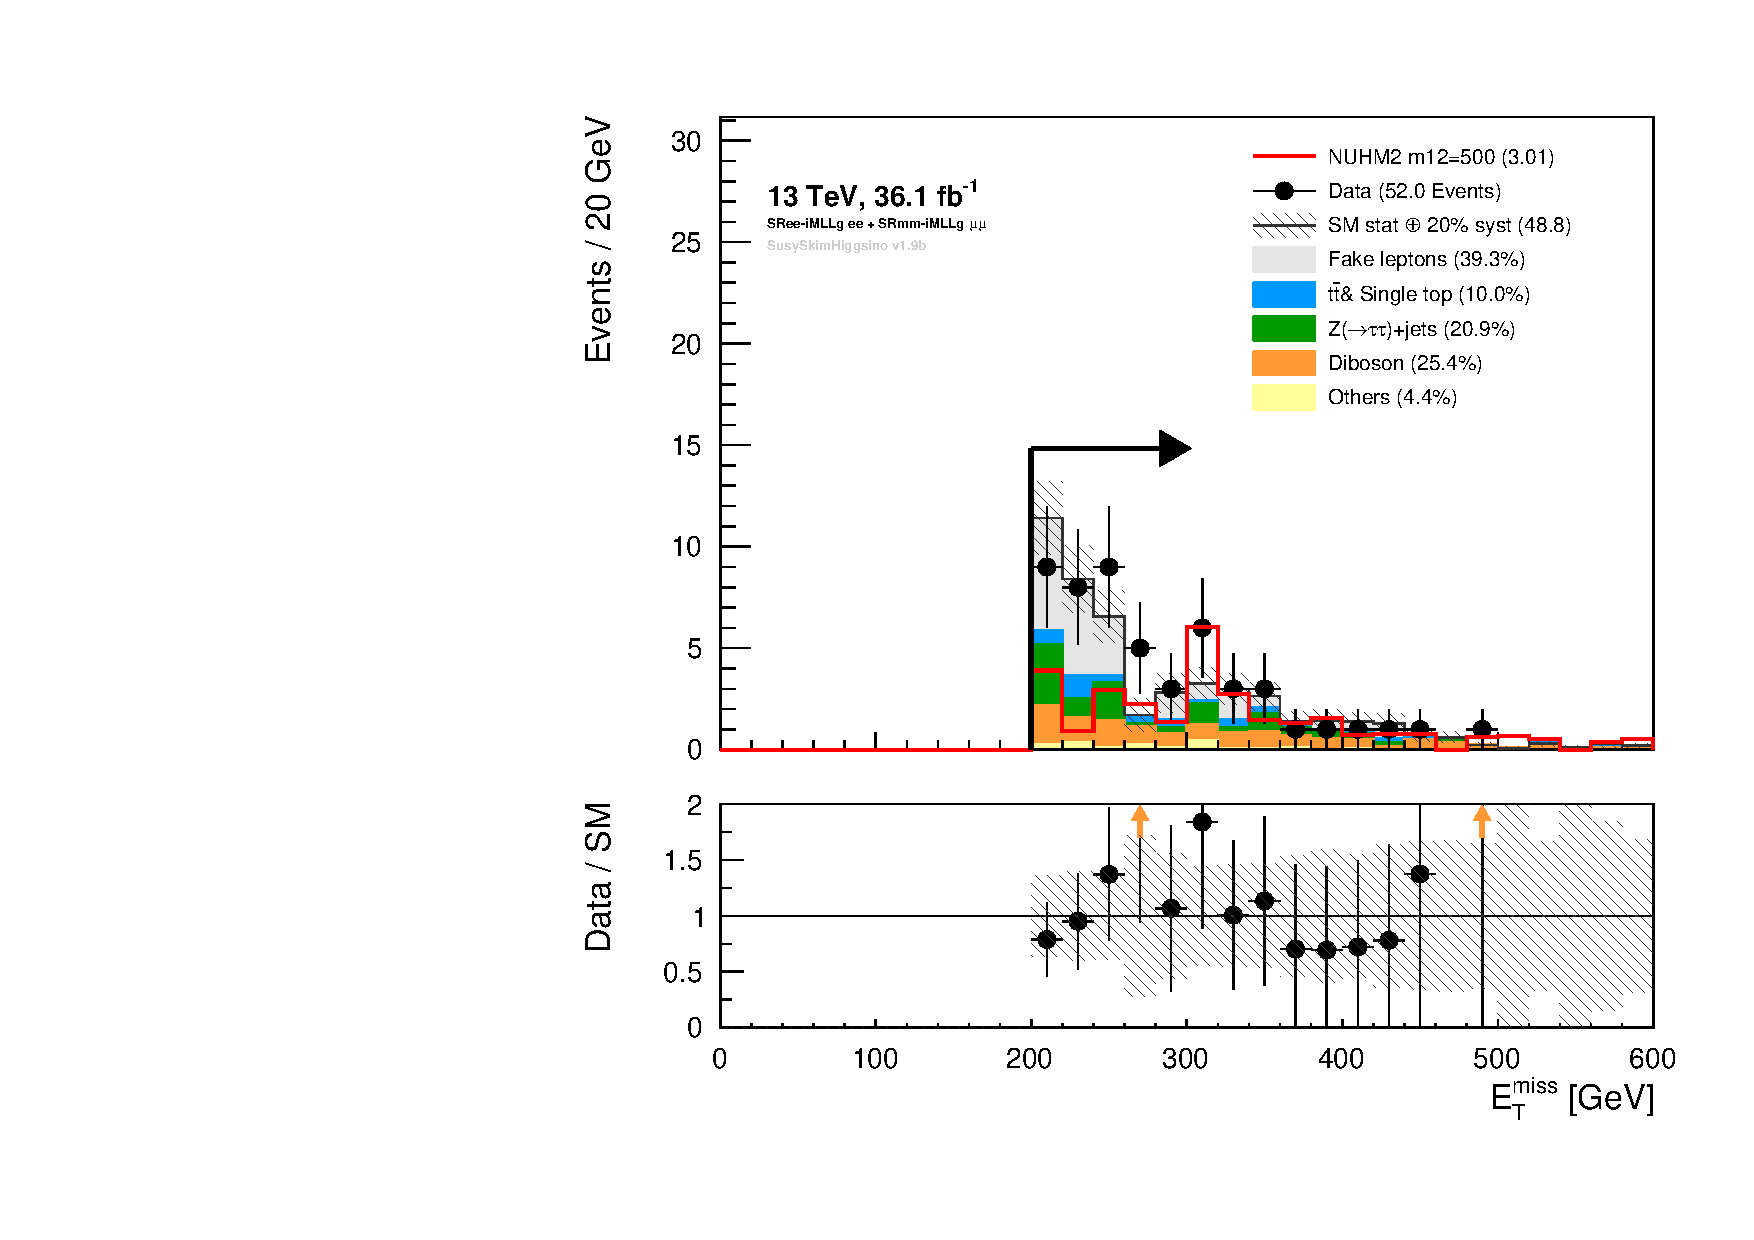
\includegraphics[scale=0.3]{NUHM2_m12_500_and_Bkg_met_Et_SFOS_N_minus_one_distribution_in_SR_times_10_on_Nsig.pdf}
%             \caption{$E^{\mathrm{miss}}_{\mathrm{T}}$}
%             \label{fig:event_nuhm2_m12_500_met_SFOS}
%         \end{subfigure}
%         \begin{subfigure}[b]{0.48\textwidth}
%             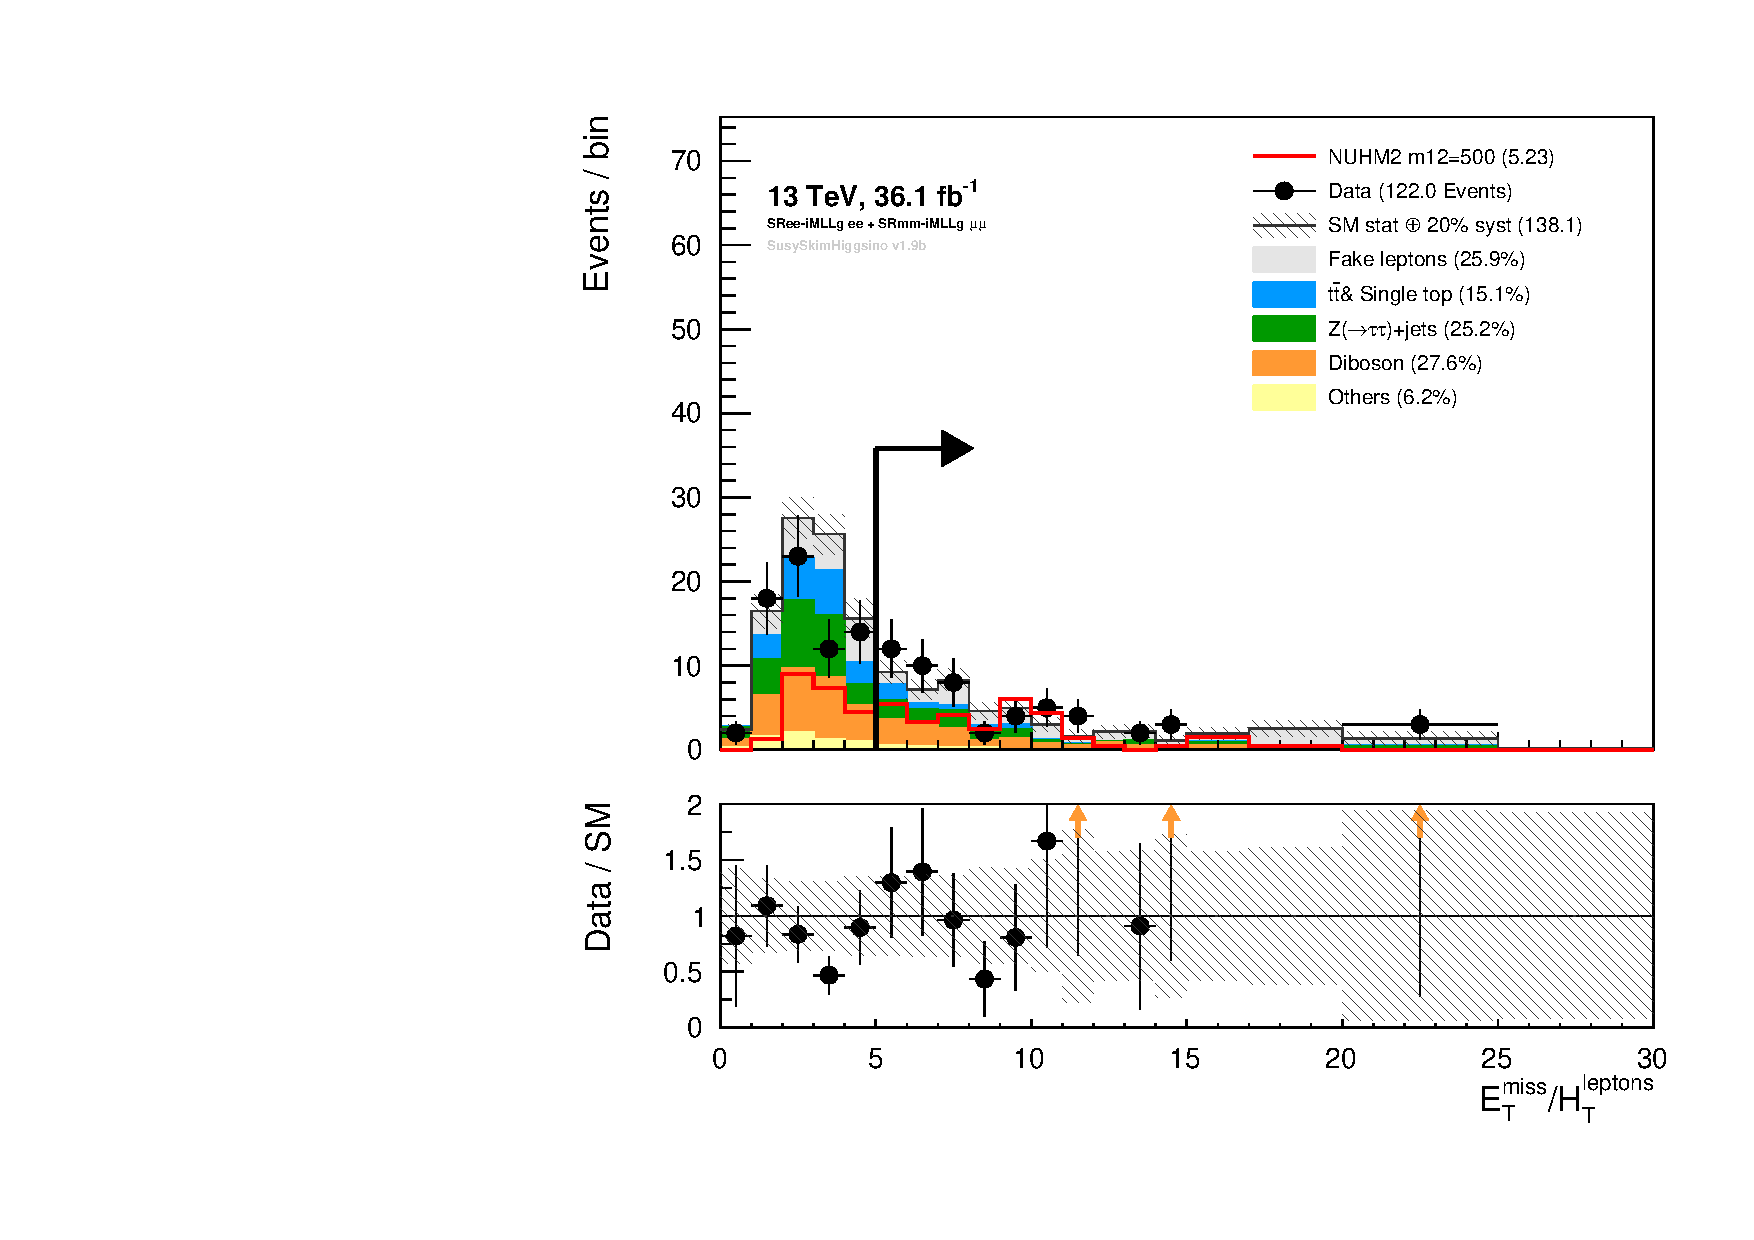
\includegraphics[scale=0.3]{NUHM2_m12_500_and_Bkg_METOverHTLep_SFOS_N_minus_one_distribution_in_SR_times_10_on_Nsig.pdf}
%             \caption{$E^{\mathrm{miss}}_{\mathrm{T}} / H^{\mathrm{leptons}}_{\mathrm{T}}$}
%             \label{fig:event_nuhm2_m12_500_METOverHTLep_SFOS}
%         \end{subfigure}
%     \end{center}
%     \caption{The `$N-1$' distributions for NUHM2 model with $m_{1/2} = 500$~{\GeV} in SR region $1 < $SR$\ell \ell$-$m_{\ell \ell} < 60$~{\GeV}.
%     The NUHM2 distributions are multiplied by 10 but the number of events in the legend use its actual values.}
%     \label{fig:dist_nuhm2_kinematic_in_SR_SFOS_m12_500_1}
% \end{figure}

% \begin{figure}[htbp]
%     \begin{center}
%         \begin{subfigure}[b]{0.48\textwidth}
%             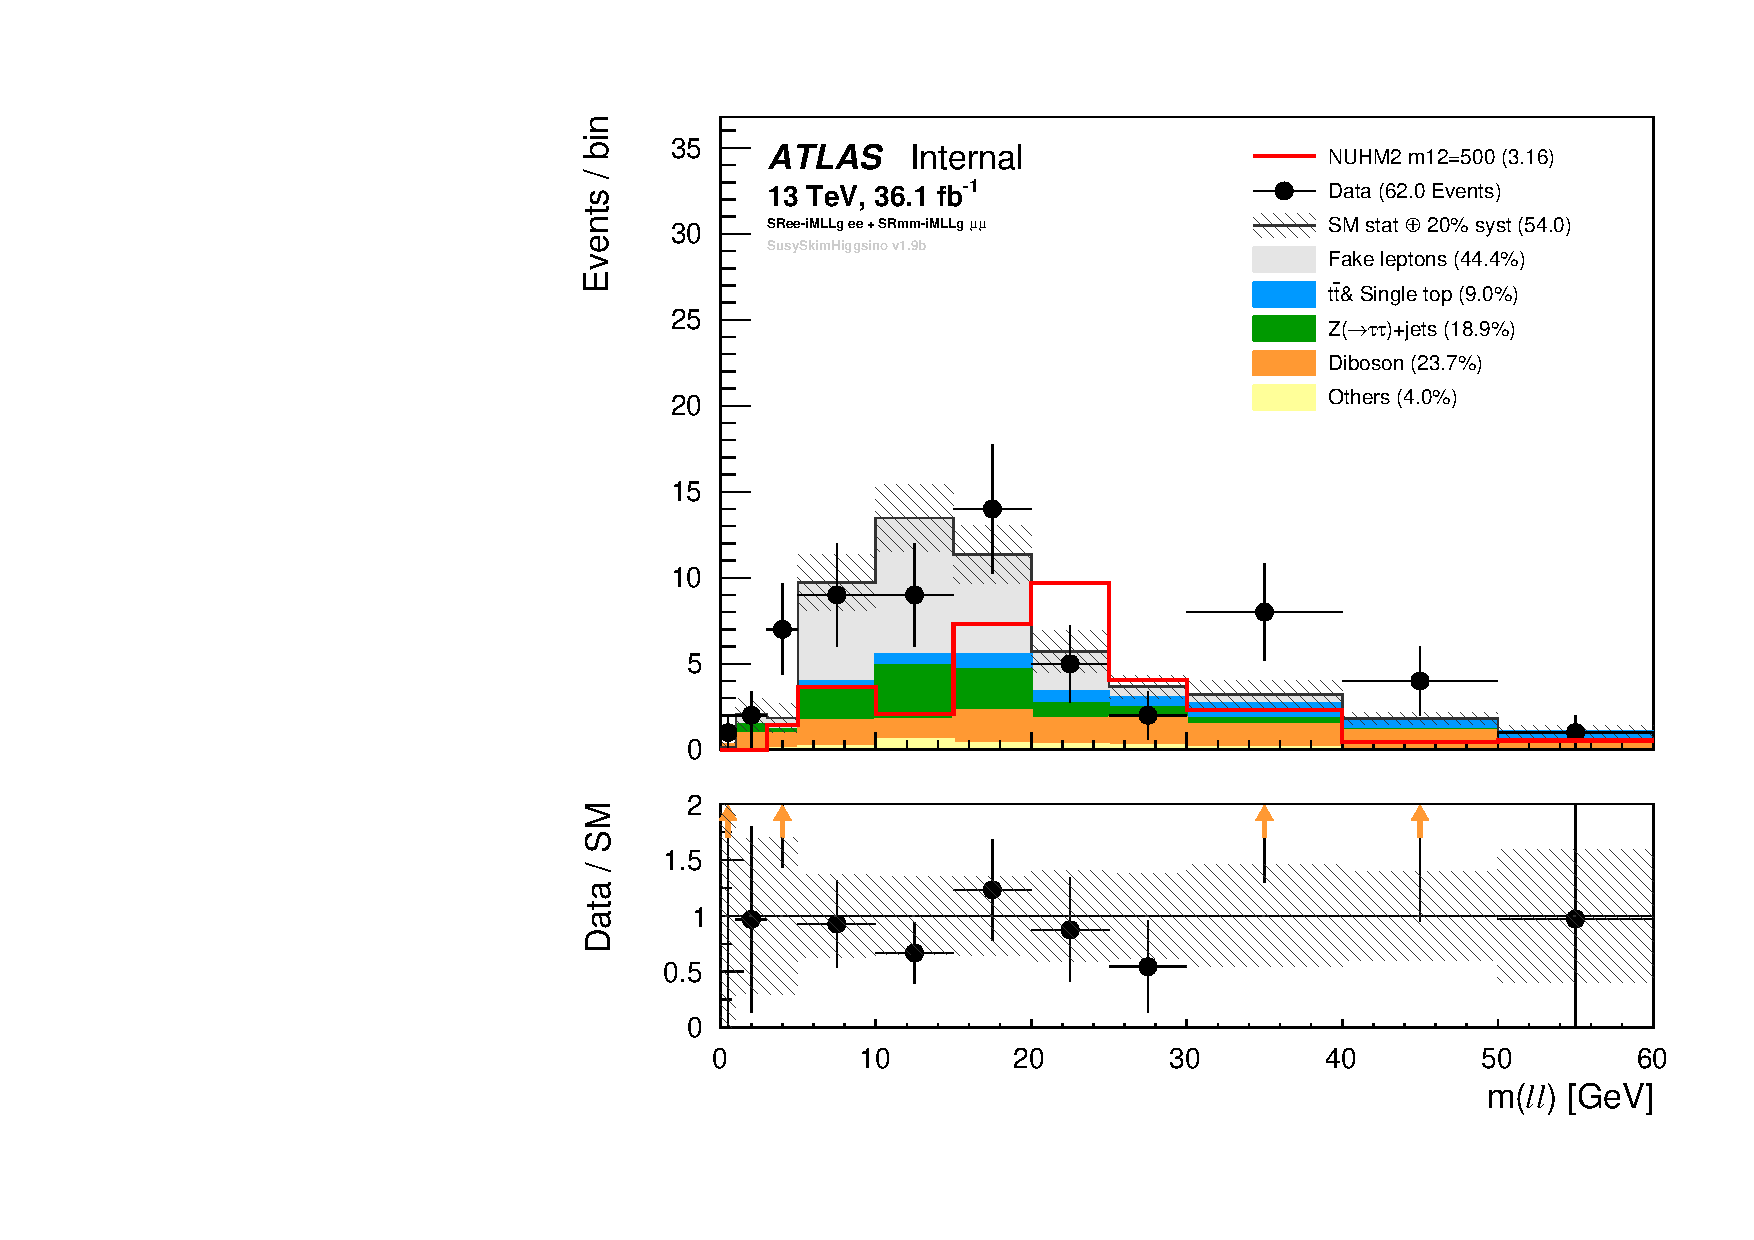
\includegraphics[scale=0.3]{NUHM2_m12_500_and_Bkg_mll_SFOS_N_minus_one_distribution_in_SR_times_10_on_Nsig.pdf}
%             \caption{$m_{\ell\ell}$}
%             \label{fig:event_nuhm2_m12_500_mll_SFOS}
%         \end{subfigure}
%         \begin{subfigure}[b]{0.48\textwidth}
%             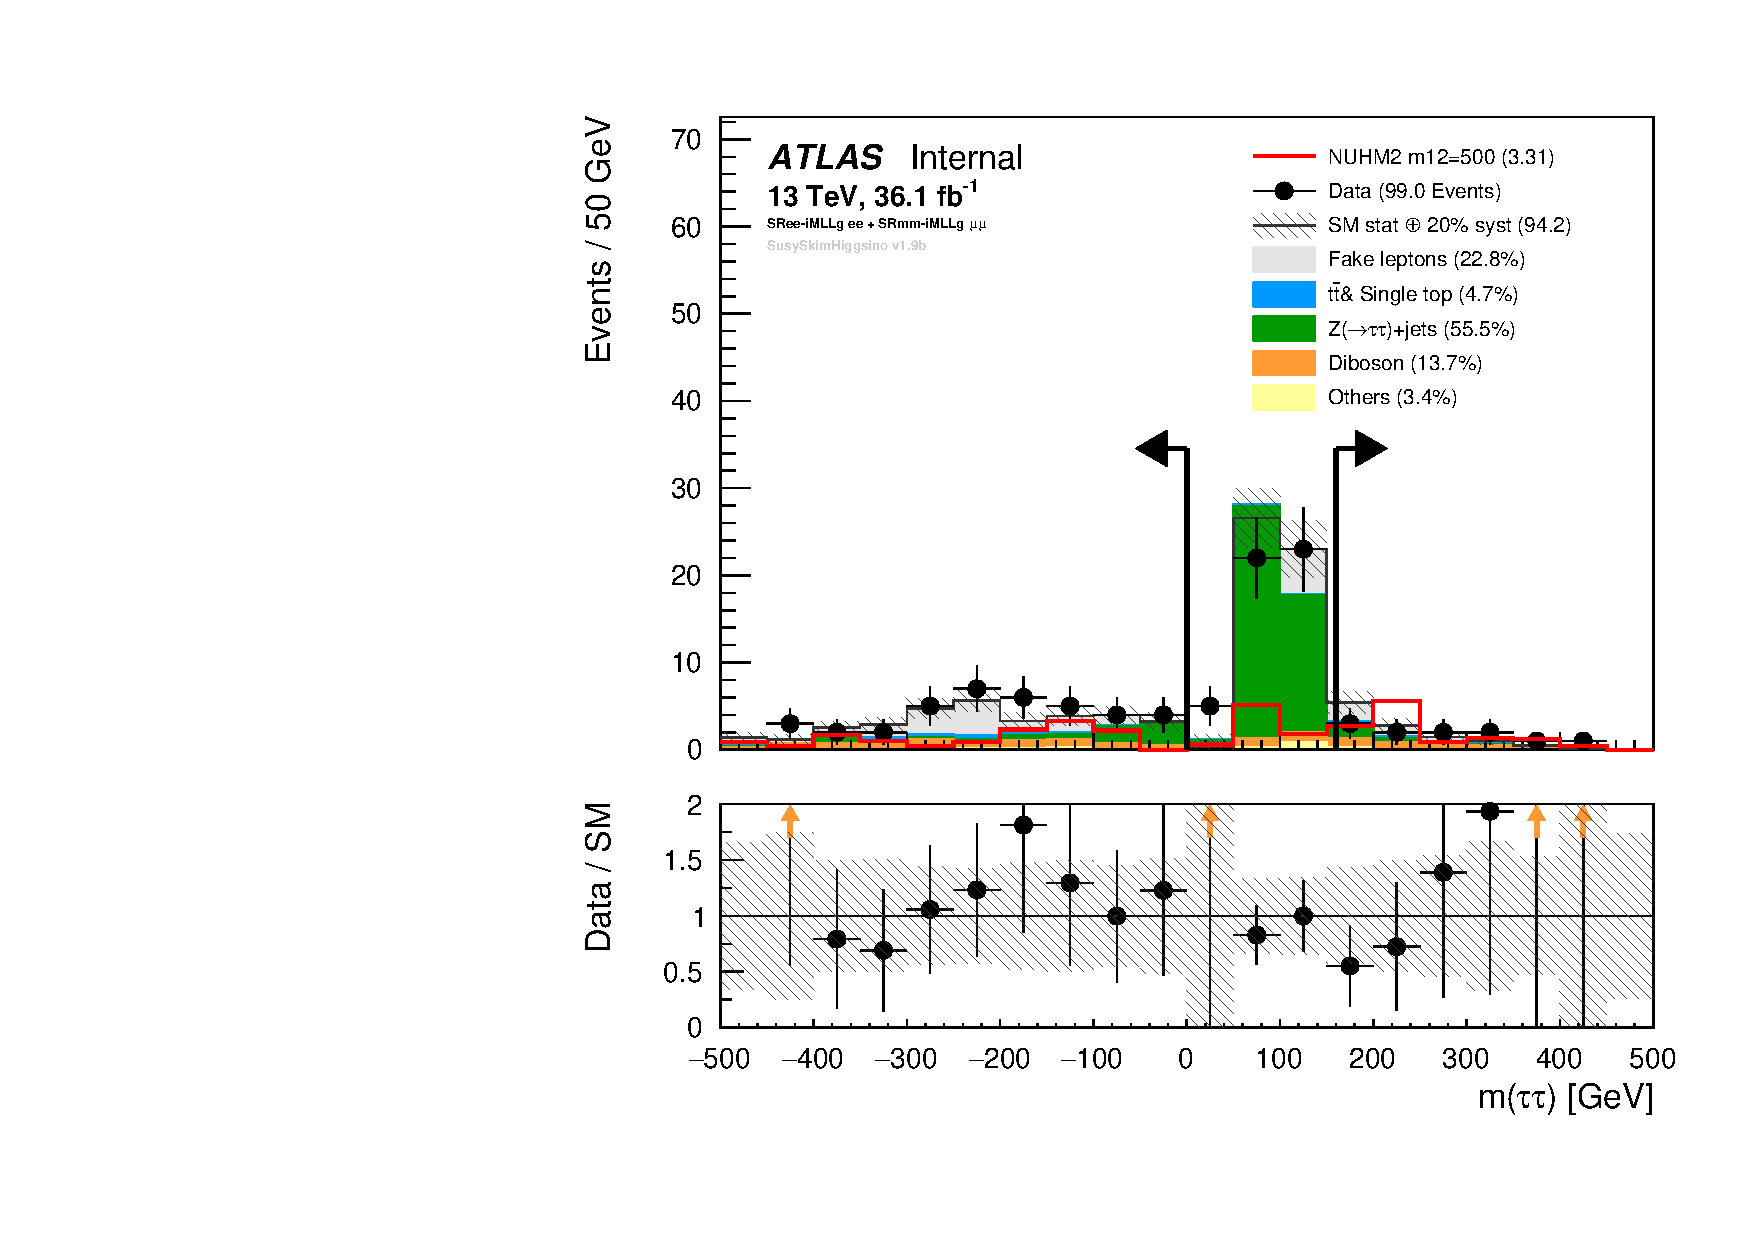
\includegraphics[scale=0.3]{NUHM2_m12_500_and_Bkg_MTauTau_SFOS_N_minus_one_distribution_in_SR_times_10_on_Nsig.pdf}
%             \caption{$m_{\tau\tau}$}
%             \label{fig:event_nuhm2_m12_500_MTauTau_SFOS}
%         \end{subfigure}
%         \begin{subfigure}[b]{0.48\textwidth}
%             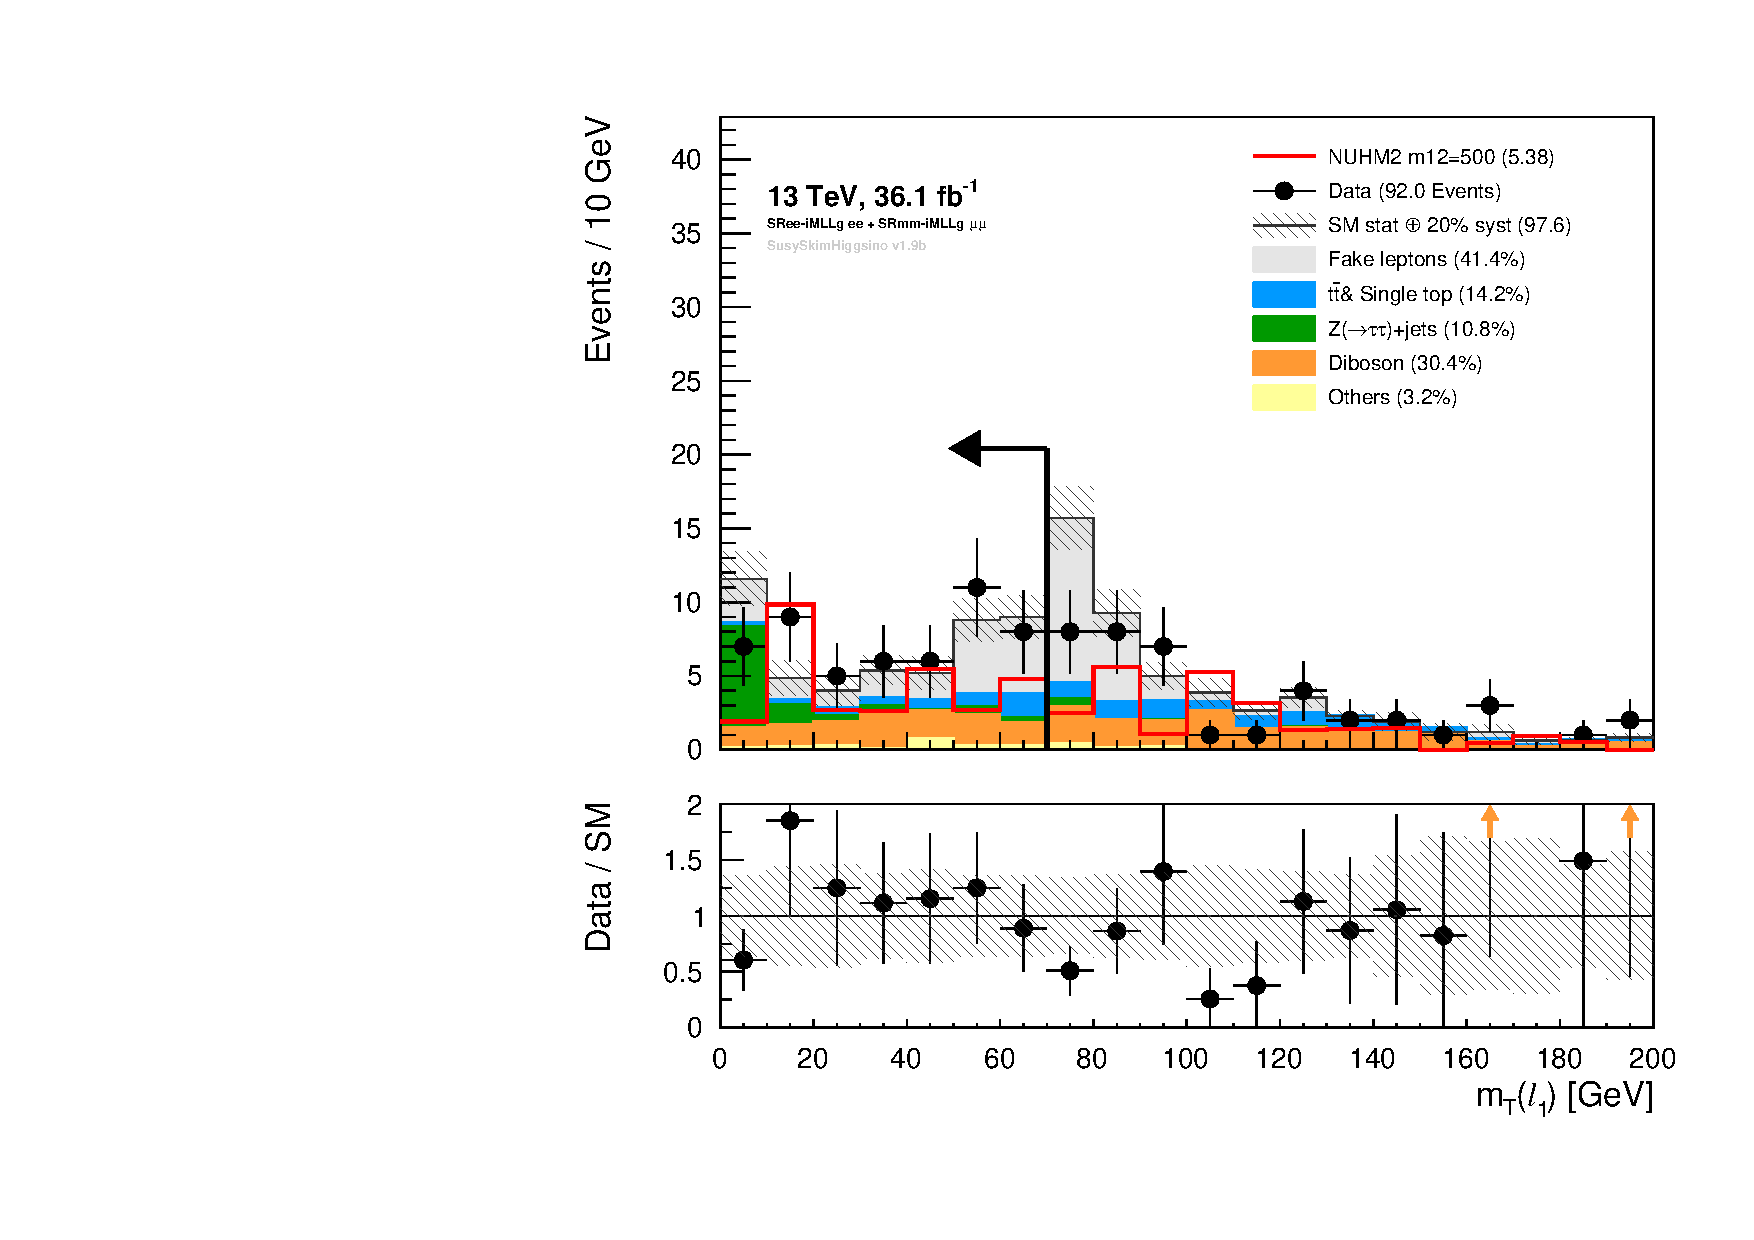
\includegraphics[scale=0.3]{NUHM2_m12_500_and_Bkg_mt_lep1_SFOS_N_minus_one_distribution_in_SR_times_10_on_Nsig.pdf}
%             \caption{$m_{T}(\ell_{1})$}
%             \label{fig:event_nuhm2_m12_500_mt_lep1_SFOS}
%         \end{subfigure}
%         \begin{subfigure}[b]{0.48\textwidth}
%             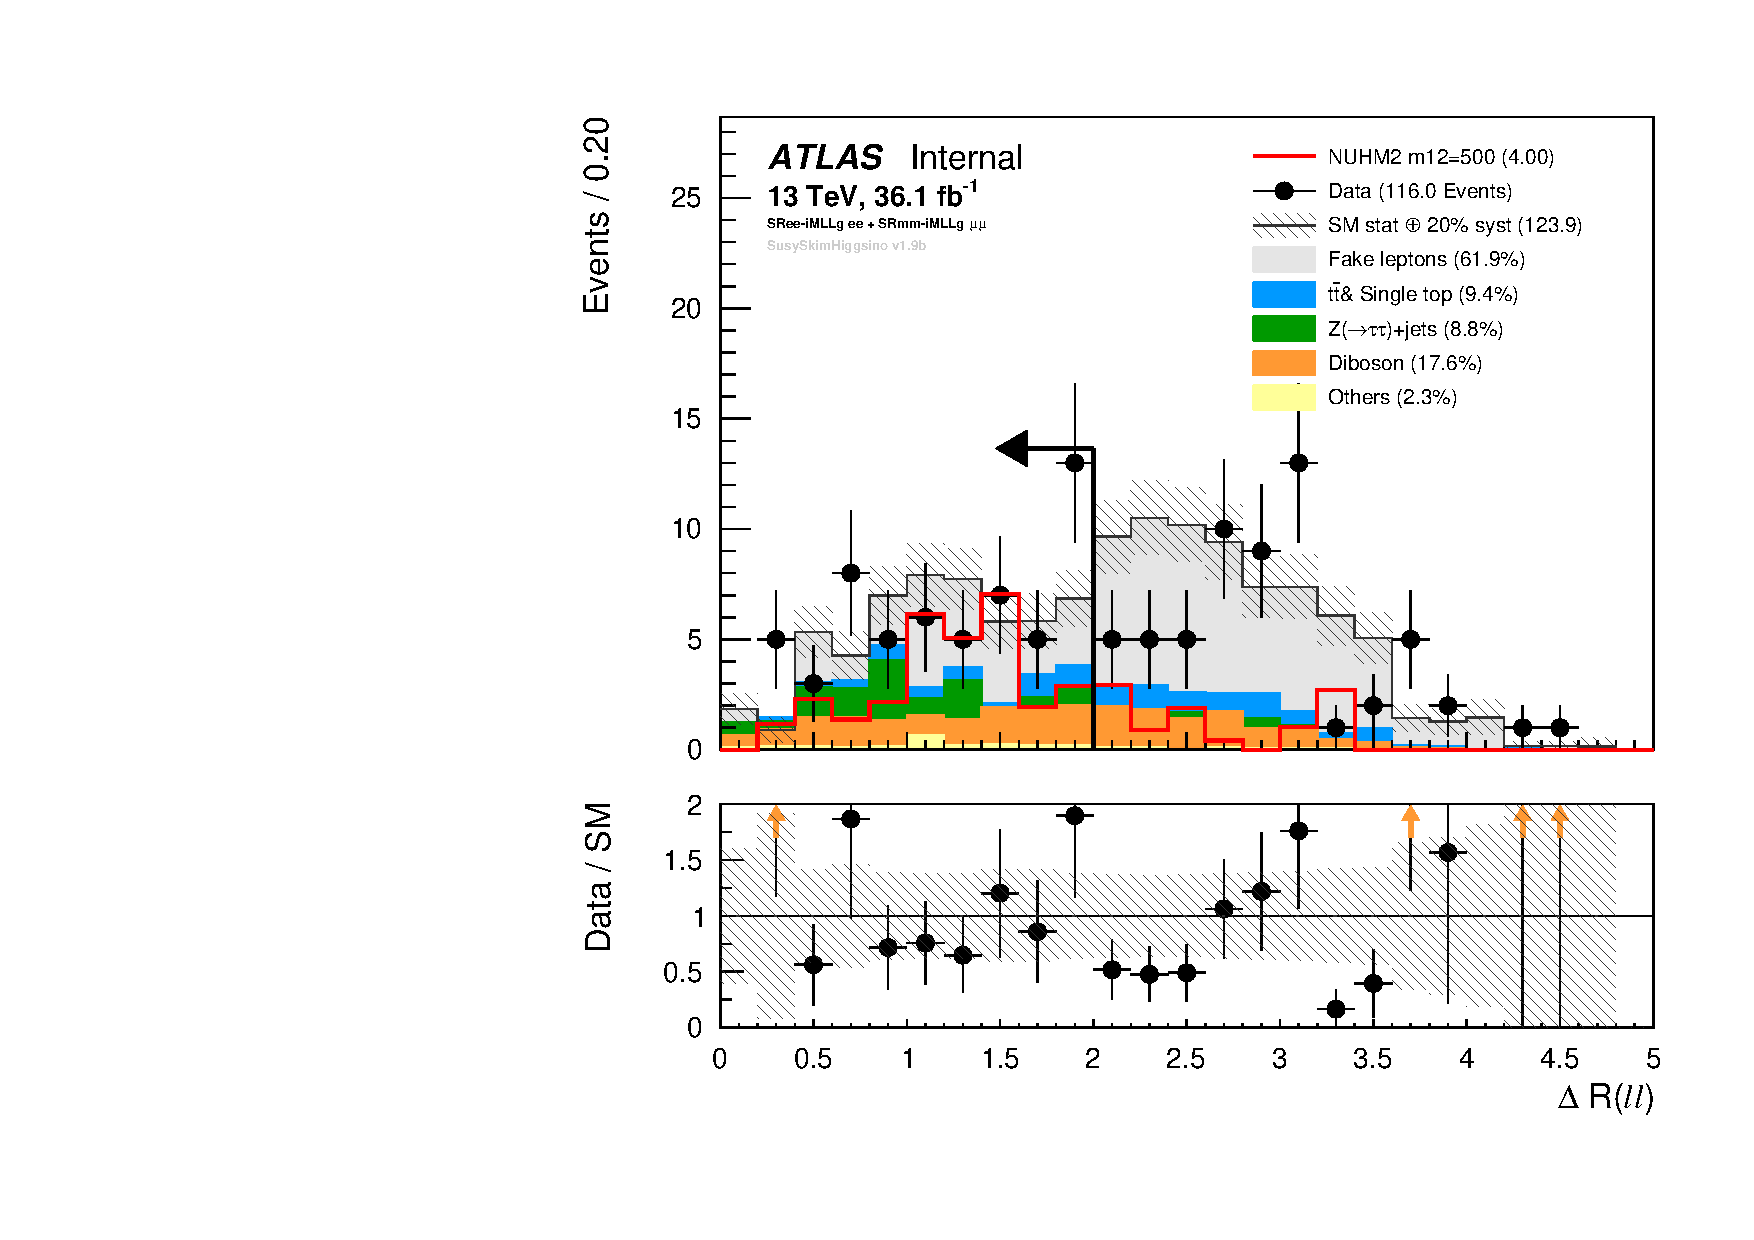
\includegraphics[scale=0.3]{NUHM2_m12_500_and_Bkg_Rll_SFOS_N_minus_one_distribution_in_SR_times_10_on_Nsig.pdf}
%             \caption{$\Delta R_{\ell\ell}$}
%             \label{fig:event_nuhm2_m12_500_Rll_SFOS}
%         \end{subfigure}
%         \begin{subfigure}[b]{0.48\textwidth}
%             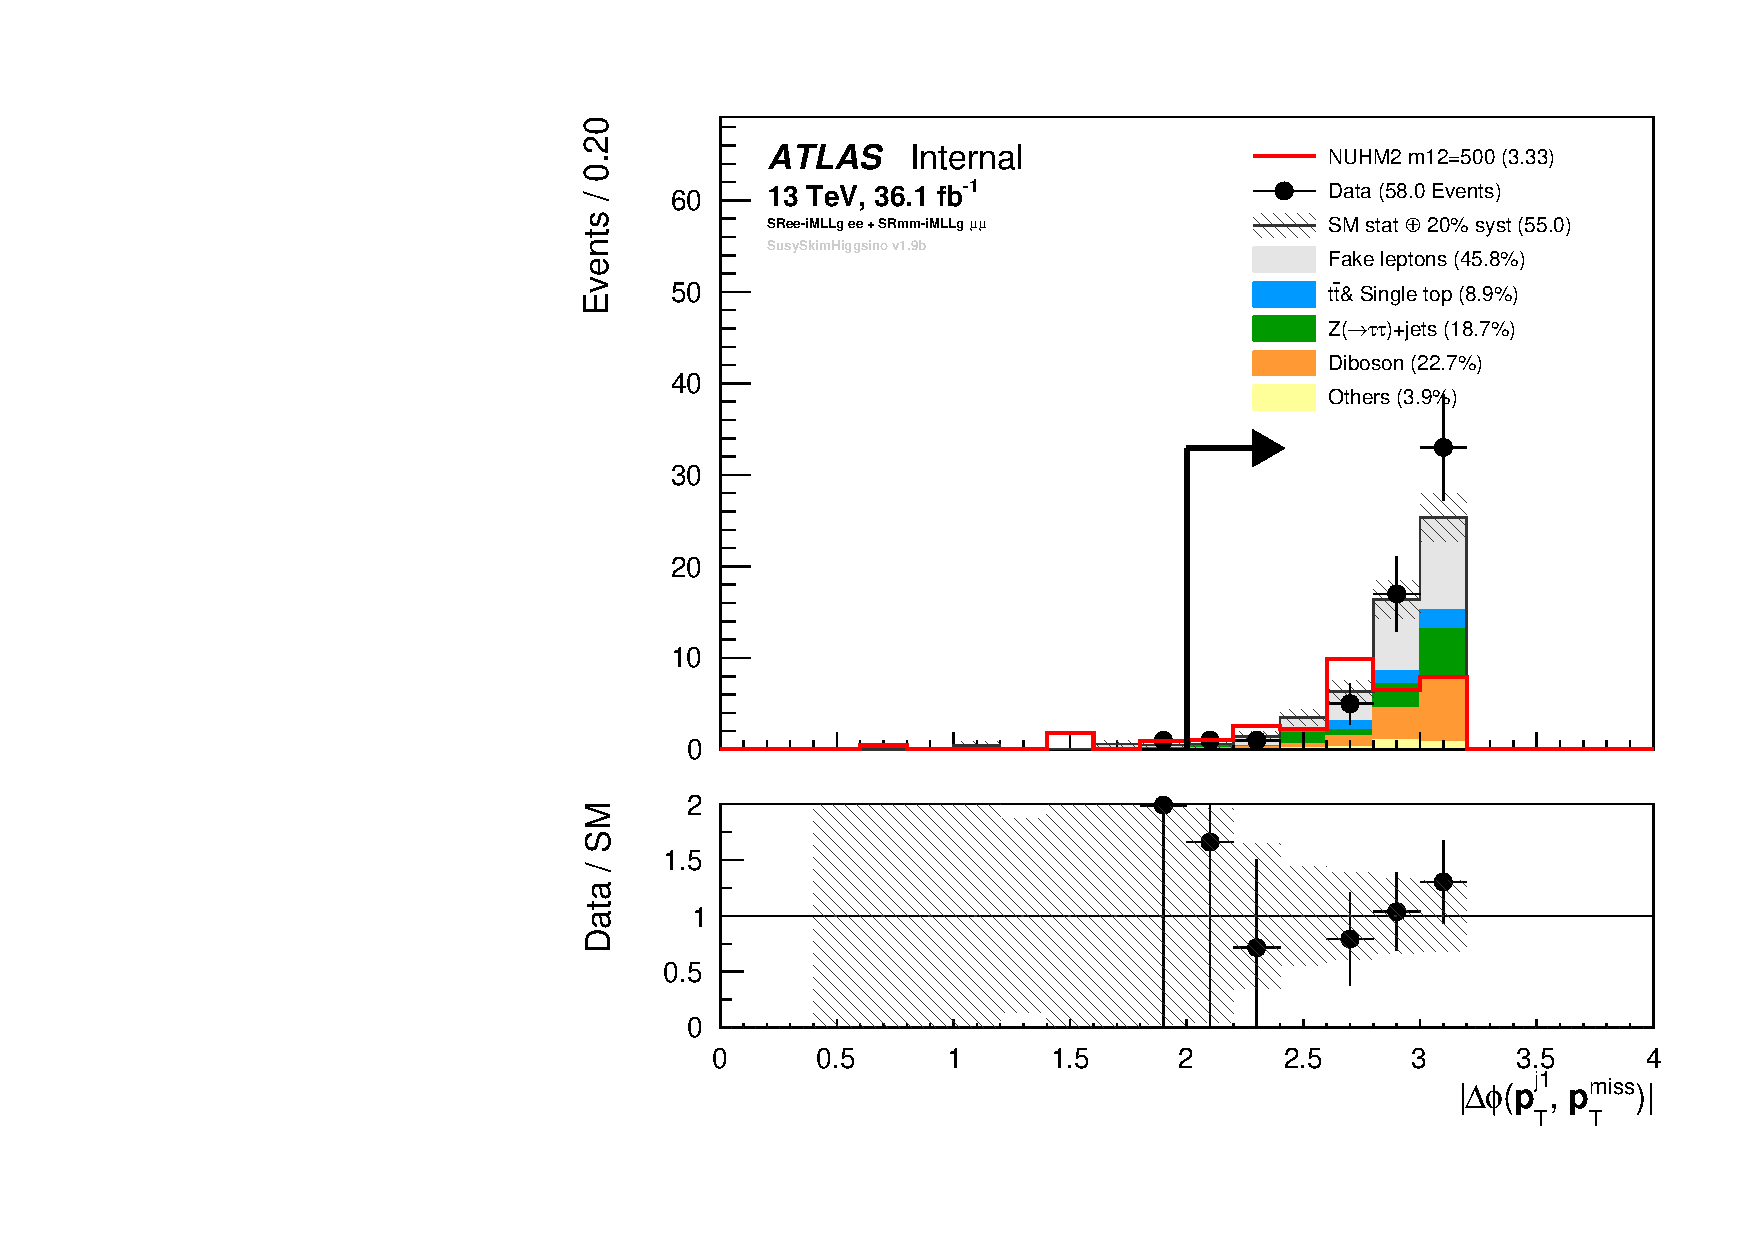
\includegraphics[scale=0.3]{NUHM2_m12_500_and_Bkg_DPhiJ1Met_SFOS_N_minus_one_distribution_in_SR_times_10_on_Nsig.pdf}
%             \caption{$|\Delta \phi(\mathbf{p}^{j_{1}}_{\mathrm{T}}, \mathbf{p}^{\mathrm{miss}}_{\mathrm{T}})|$}
%             \label{fig:event_nuhm2_m12_500_DPhiJ1Met_SFOS}
%         \end{subfigure}
%         \begin{subfigure}[b]{0.48\textwidth}
%             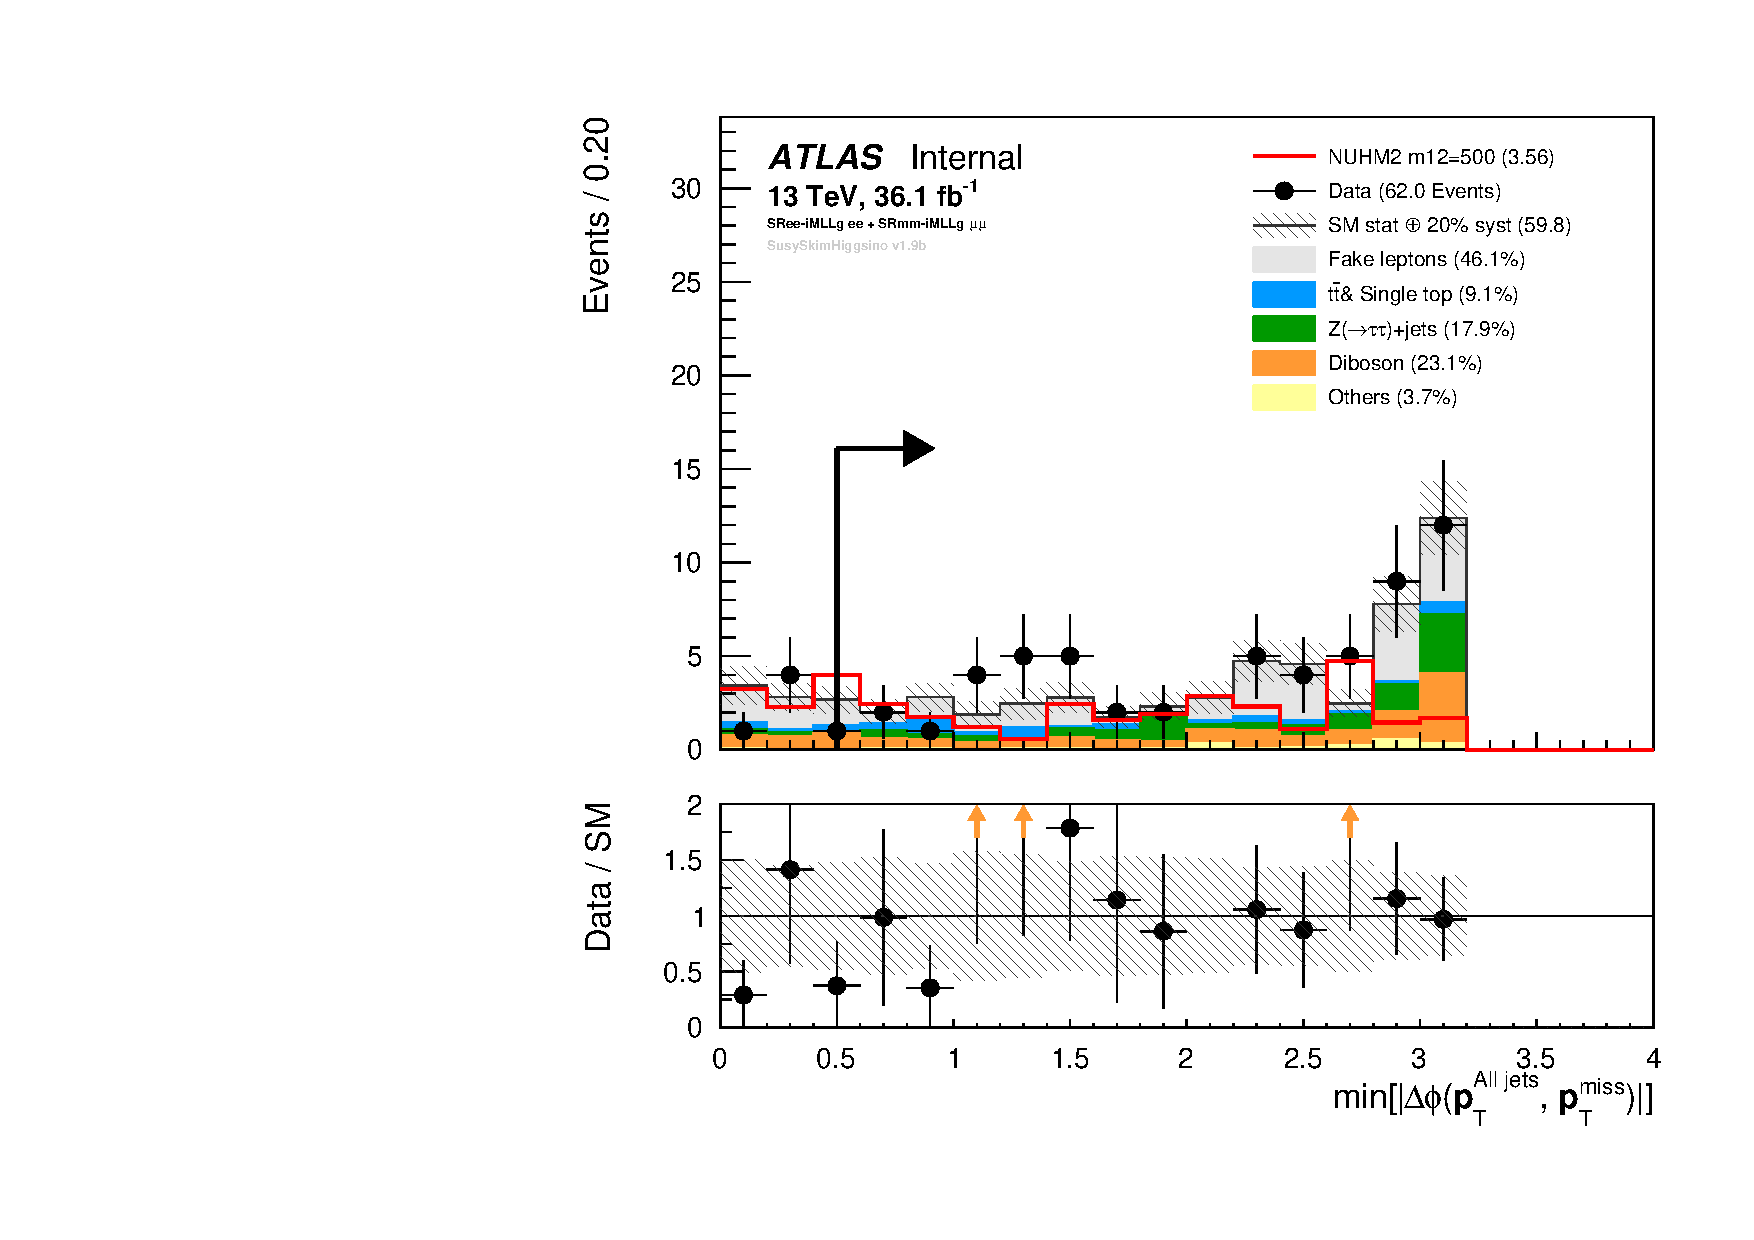
\includegraphics[scale=0.3]{NUHM2_m12_500_and_Bkg_minDPhiAllJetsMet_SFOS_N_minus_one_distribution_in_SR_times_10_on_Nsig.pdf}
%             \caption{min[$|\Delta \phi(\mathbf{p}^{\textrm{All jets}}_{\mathrm{T}}, \mathbf{p}^{\mathrm{miss}}_{\mathrm{T}})|$]}
%             \label{fig:event_nuhm2_m12_500_minDPhiAllJetsMet_SFOS}
%         \end{subfigure}
%     \end{center}
%     \caption{The `$N-1$' distributions for NUHM2 model with $m_{1/2} = 500$~{\GeV} in SR region $1 < $SR$\ell \ell$-$m_{\ell \ell} < 60$~{\GeV}.
%     The NUHM2 distributions are multiplied by 10 but the number of events in the legend use its actual values.}
%     \label{fig:dist_nuhm2_kinematic_in_SR_SFOS_m12_500_2}
% \end{figure}

% m12 = 600
\begin{figure}[htbp]
    \begin{center}
        \begin{subfigure}[b]{0.48\textwidth}
            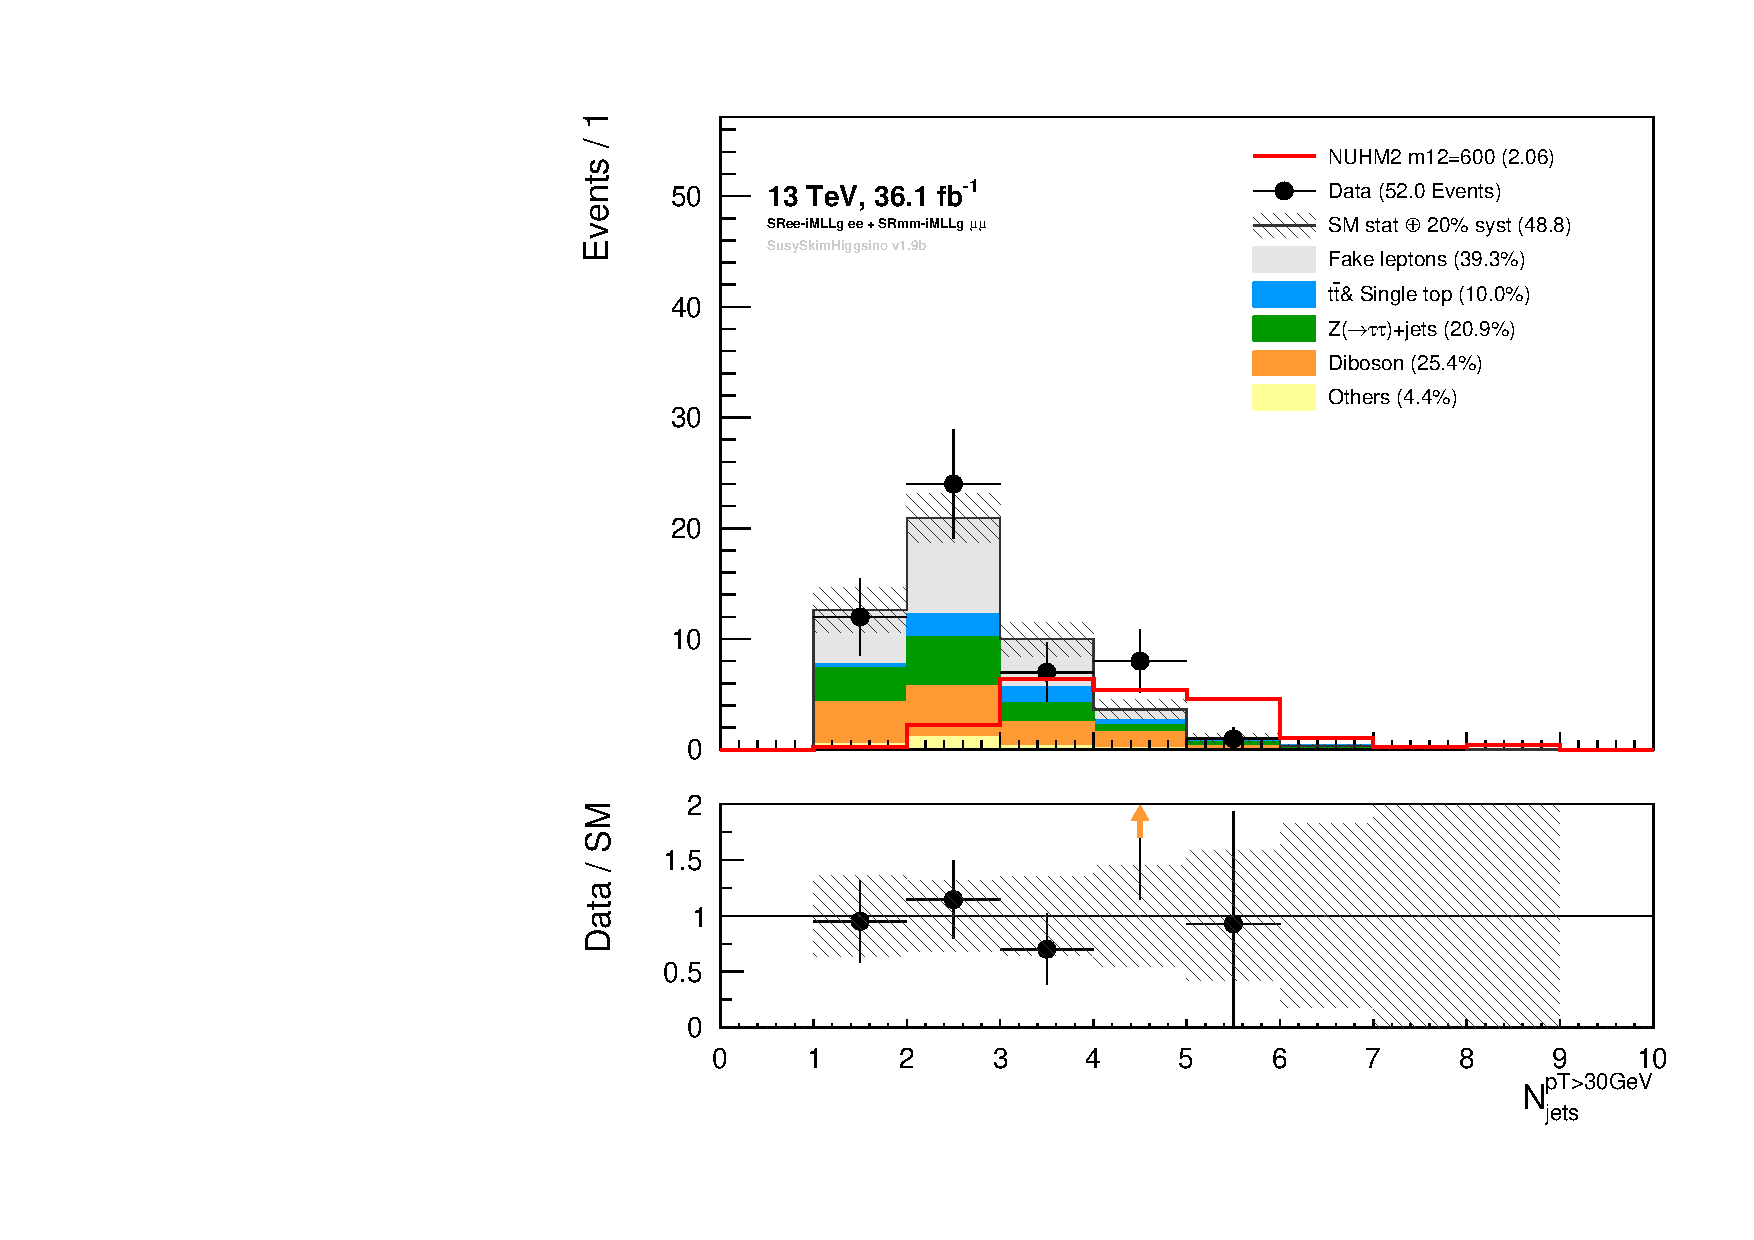
\includegraphics[scale=0.3]{NUHM2_m12_600_and_Bkg_nJet30_SFOS_N_minus_one_distribution_in_SR_times_10_on_Nsig.pdf}
            \caption{$N^{30}_{\mathrm{jets}}$}
            \label{fig:event_nuhm2_m12_600_nJet30_SFOS}
        \end{subfigure}
        \begin{subfigure}[b]{0.48\textwidth}
            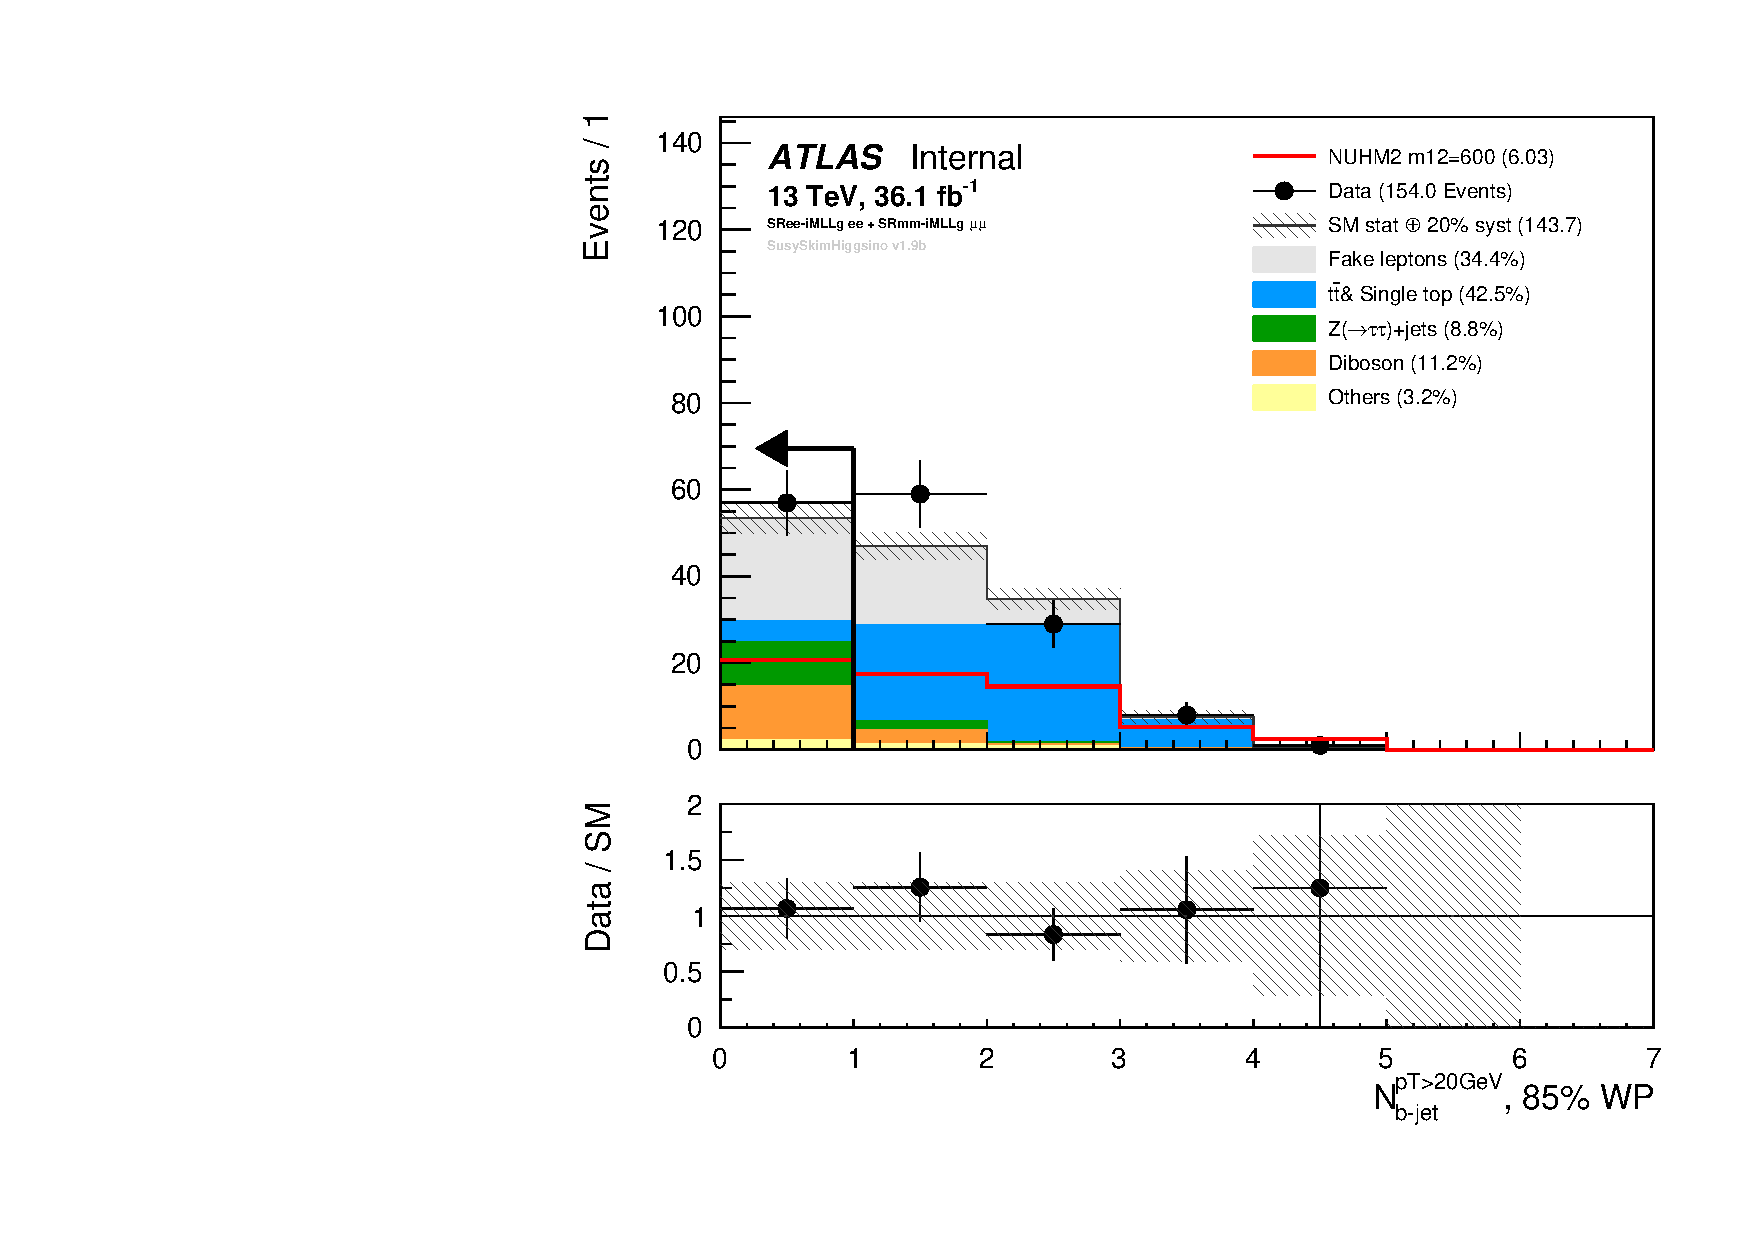
\includegraphics[scale=0.3]{NUHM2_m12_600_and_Bkg_nBJet20_MV2c10_SFOS_N_minus_one_distribution_in_SR_times_10_on_Nsig.pdf}
            \caption{$N^{20}_{\mathrm{b-jets}}$}
            \label{fig:event_nuhm2_m12_600_nBJet20_SFOS}
        \end{subfigure}
        \begin{subfigure}[b]{0.48\textwidth}
            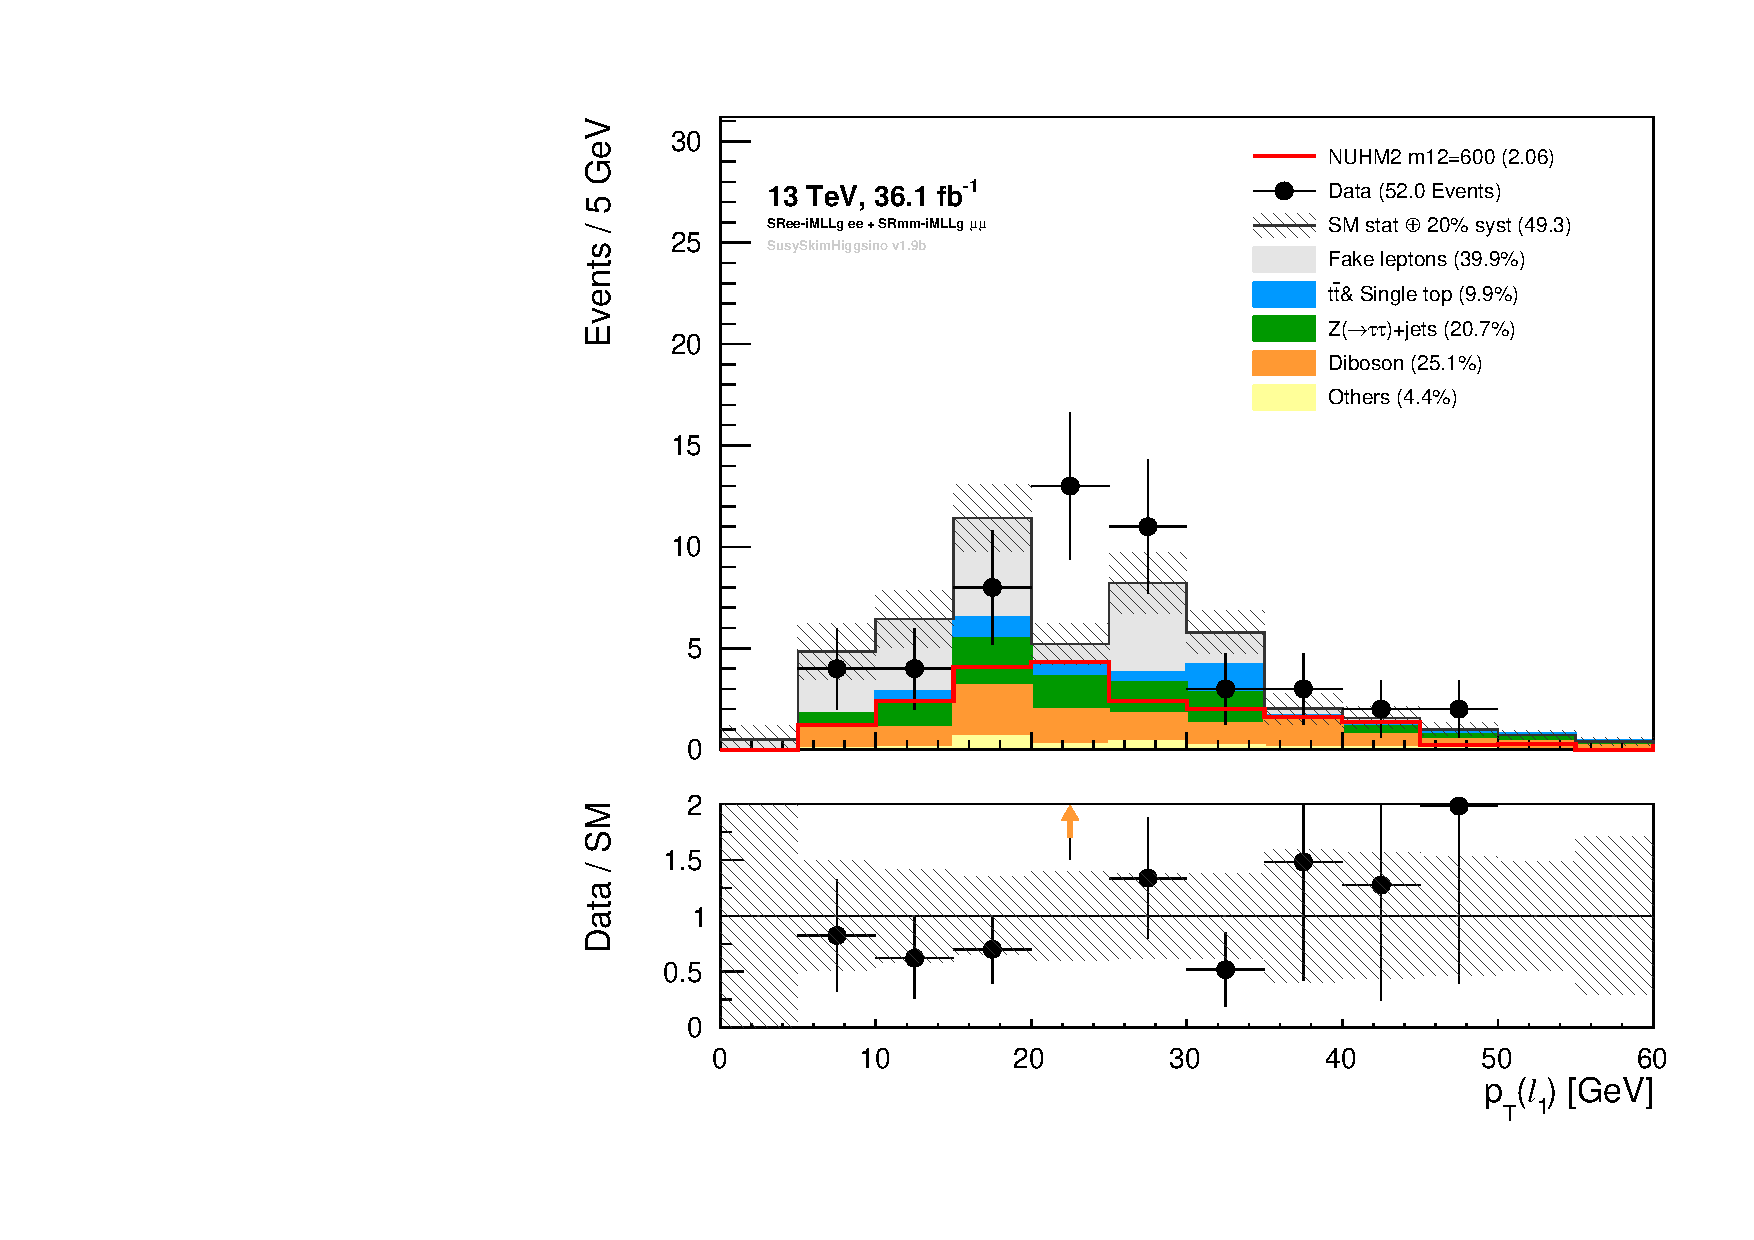
\includegraphics[scale=0.3]{NUHM2_m12_600_and_Bkg_lep1Pt_SFOS_N_minus_one_distribution_in_SR_times_10_on_Nsig.pdf}
            \caption{$p^{\ell_1}_{\mathrm{T}}$}
            \label{fig:event_nuhm2_m12_600_lep1Pt_SFOS}
        \end{subfigure}
        \begin{subfigure}[b]{0.48\textwidth}
            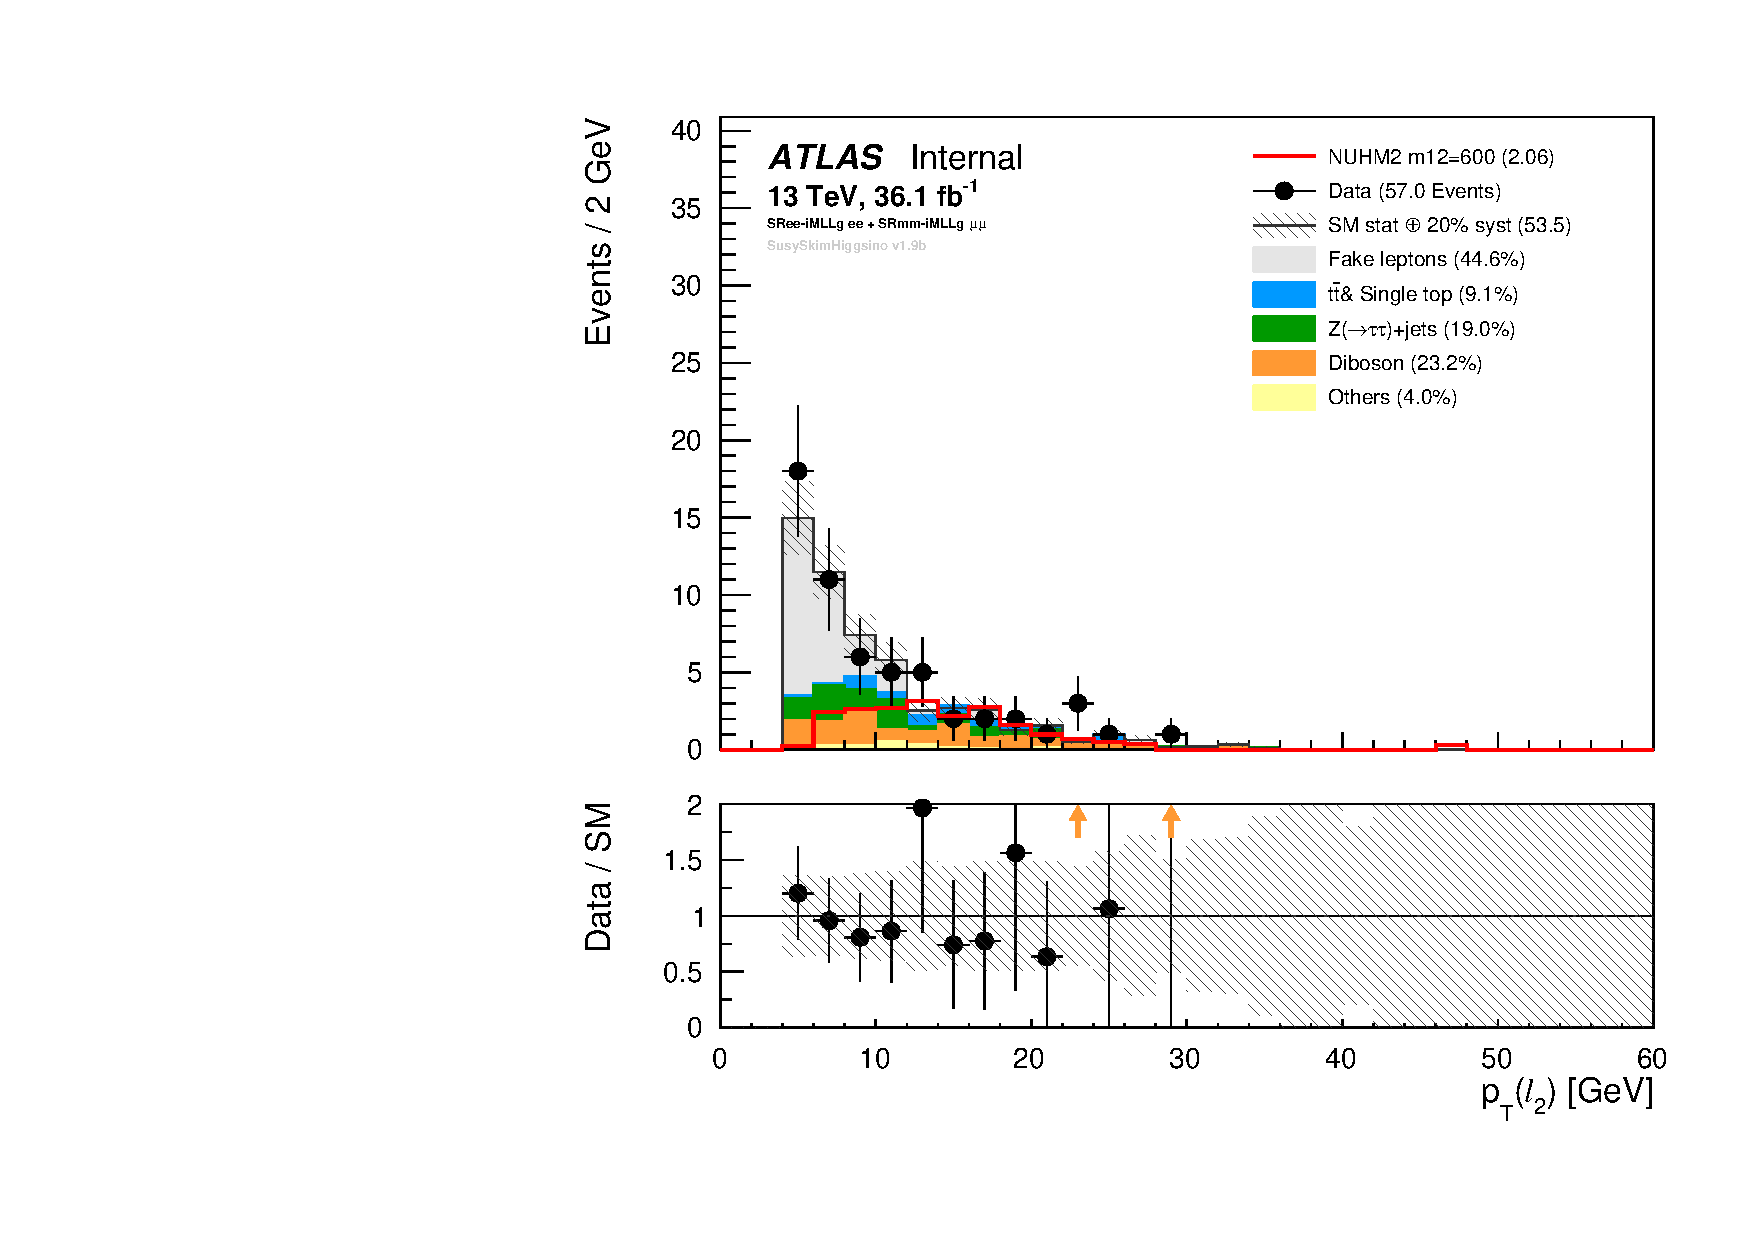
\includegraphics[scale=0.3]{NUHM2_m12_600_and_Bkg_lep2Pt_SFOS_N_minus_one_distribution_in_SR_times_10_on_Nsig.pdf}
            \caption{$p^{\ell_2}_{\mathrm{T}}$}
            \label{fig:event_nuhm2_m12_600_lep2Pt_SFOS}
        \end{subfigure}
        \begin{subfigure}[b]{0.48\textwidth}
            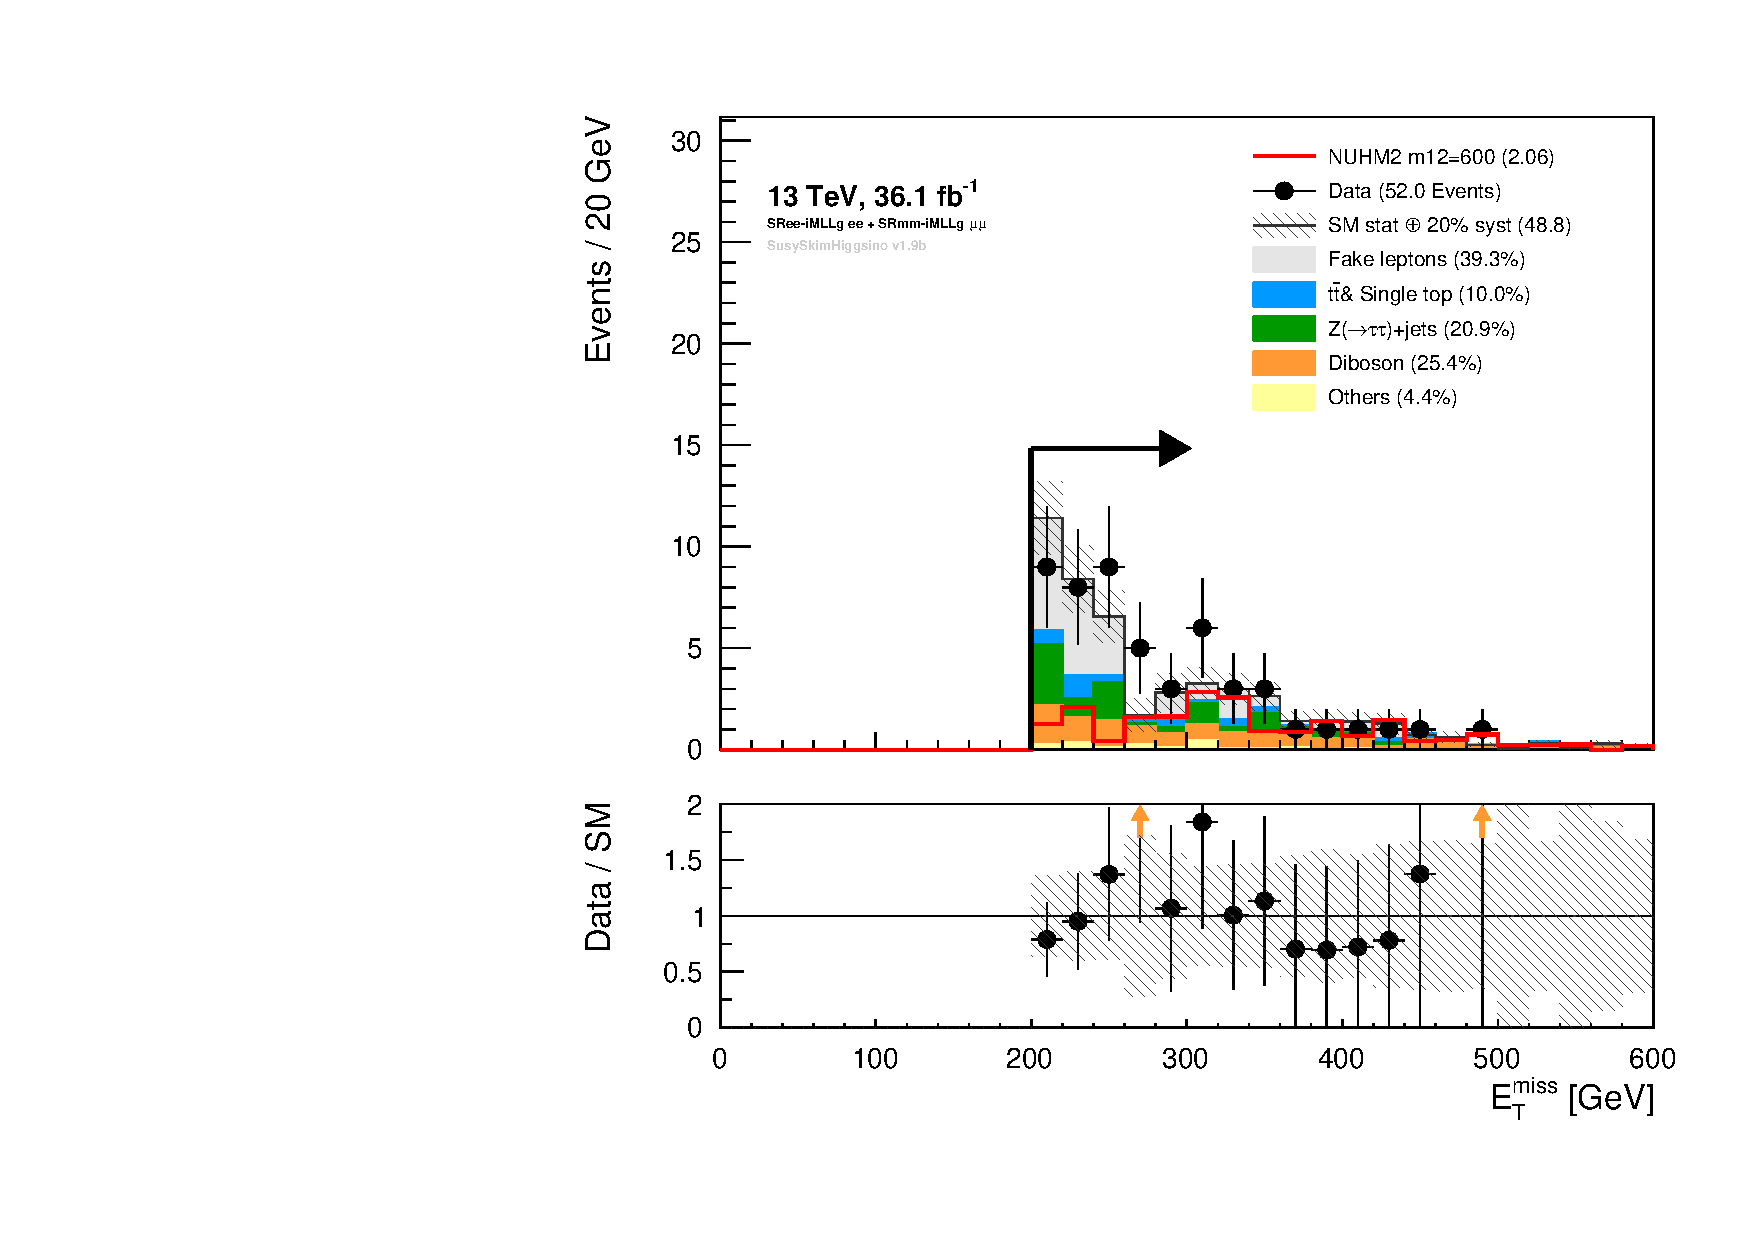
\includegraphics[scale=0.3]{NUHM2_m12_600_and_Bkg_met_Et_SFOS_N_minus_one_distribution_in_SR_times_10_on_Nsig.pdf}
            \caption{$E^{\mathrm{miss}}_{\mathrm{T}}$}
            \label{fig:event_nuhm2_m12_600_met_SFOS}
        \end{subfigure}
        \begin{subfigure}[b]{0.48\textwidth}
            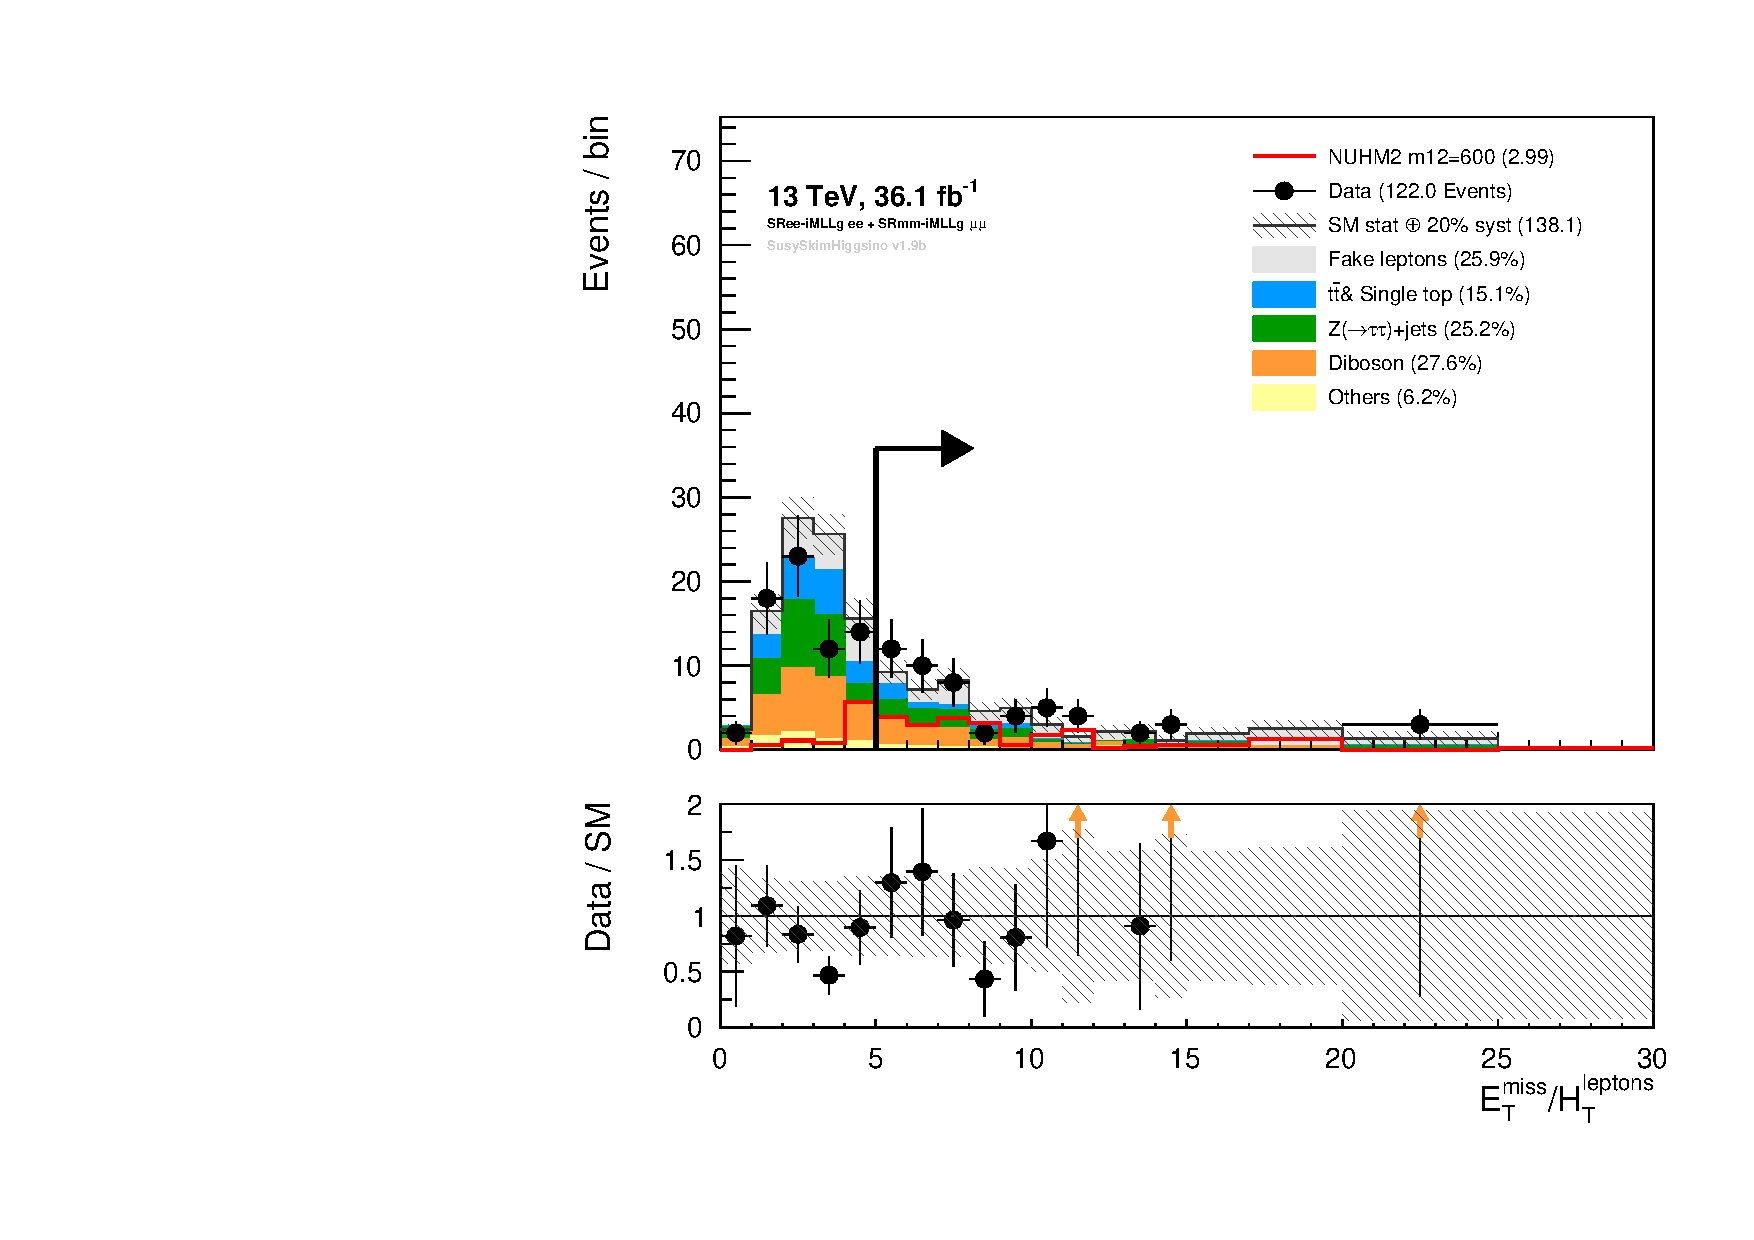
\includegraphics[scale=0.3]{NUHM2_m12_600_and_Bkg_METOverHTLep_SFOS_N_minus_one_distribution_in_SR_times_10_on_Nsig.pdf}
            \caption{$E^{\mathrm{miss}}_{\mathrm{T}} / H^{\mathrm{leptons}}_{\mathrm{T}}$}
            \label{fig:event_nuhm2_m12_600_METOverHTLep_SFOS}
        \end{subfigure}
    \end{center}
    \caption{The `$N-1$' distributions for NUHM2 model with $m_{1/2} = 600$~{\GeV} in SR region $1 < $SR$\ell \ell$-$m_{\ell \ell} < 60$~{\GeV}.
    The NUHM2 distributions are multiplied by 10 but the number of events in the legend use its actual values.}
    \label{fig:dist_nuhm2_kinematic_in_SR_SFOS_m12_600_1}
\end{figure}

\begin{figure}[htbp]
    \begin{center}
        \begin{subfigure}[b]{0.48\textwidth}
            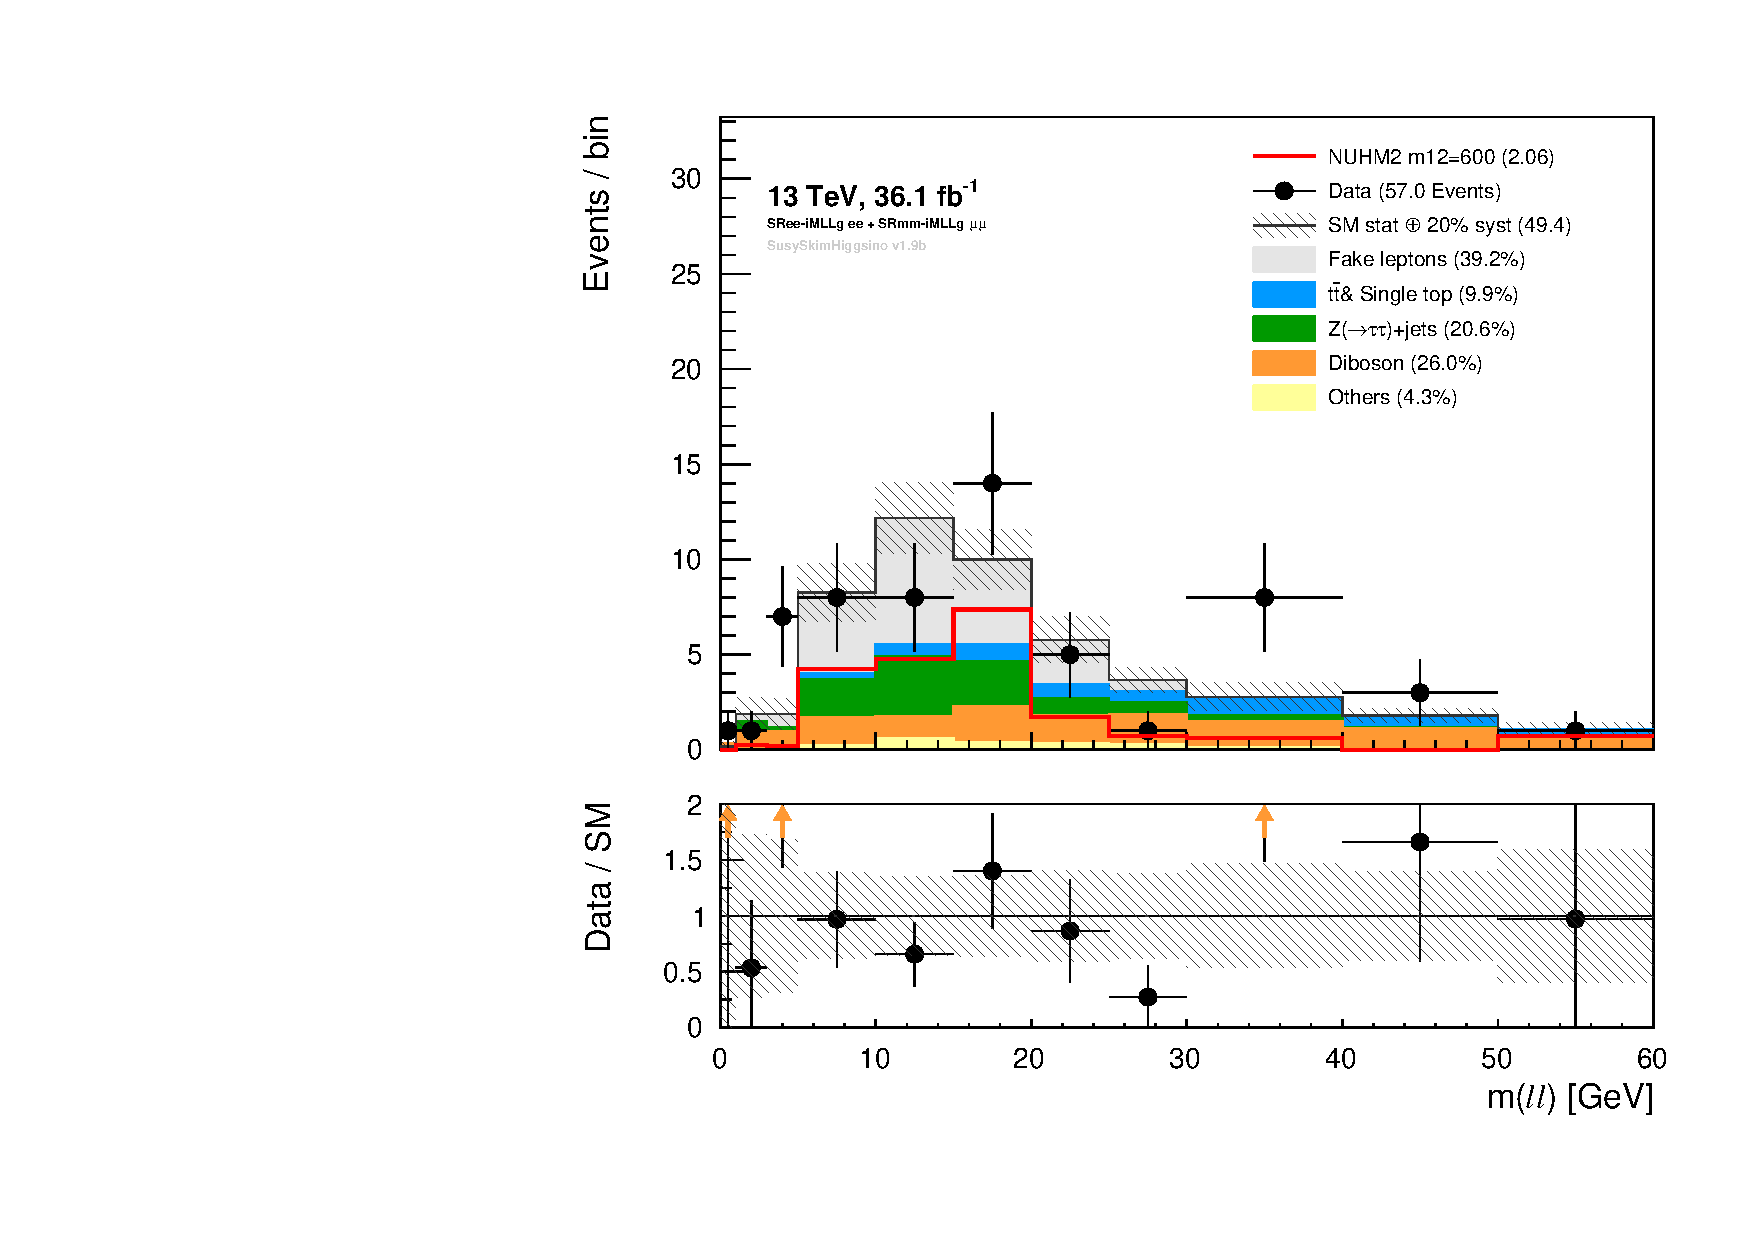
\includegraphics[scale=0.3]{NUHM2_m12_600_and_Bkg_mll_SFOS_N_minus_one_distribution_in_SR_times_10_on_Nsig.pdf}
            \caption{$m_{\ell\ell}$}
            \label{fig:event_nuhm2_m12_600_mll_SFOS}
        \end{subfigure}
        \begin{subfigure}[b]{0.48\textwidth}
            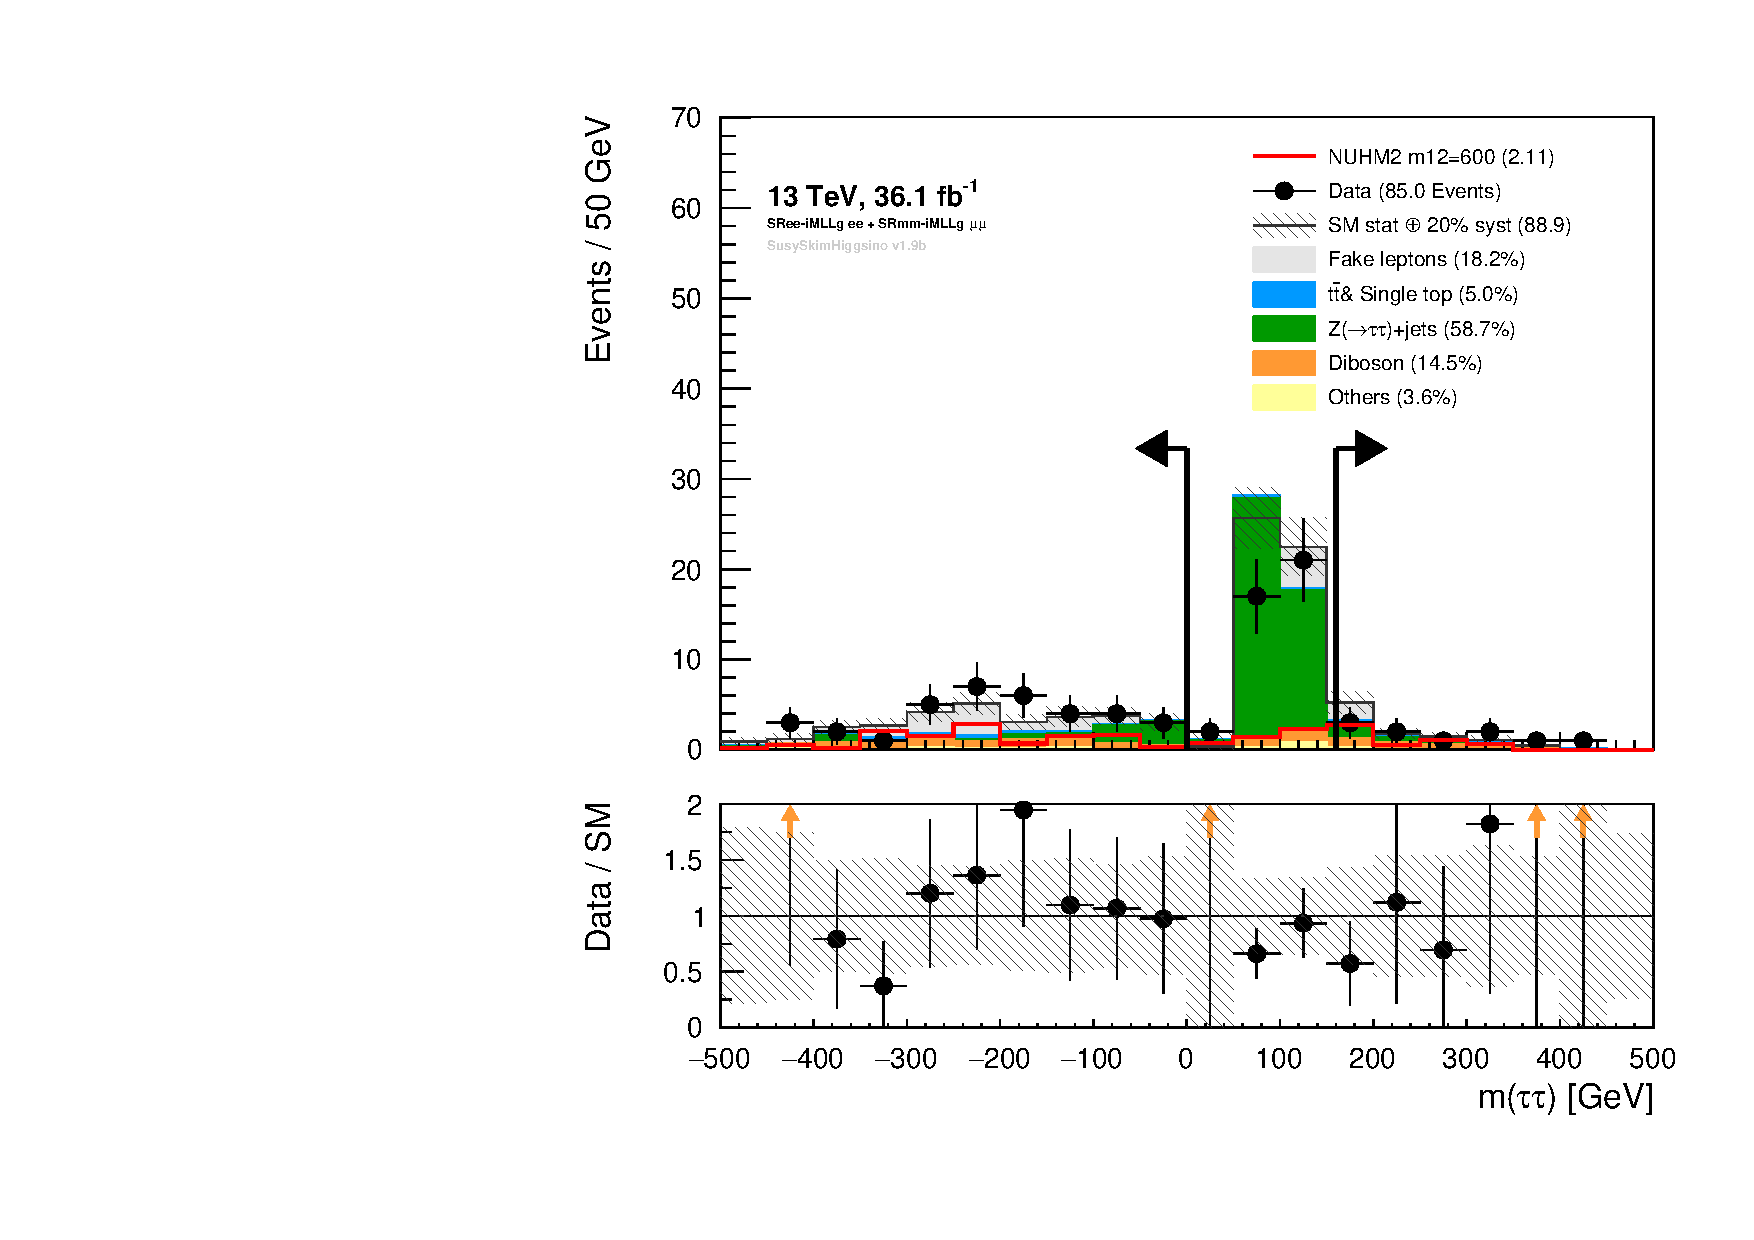
\includegraphics[scale=0.3]{NUHM2_m12_600_and_Bkg_MTauTau_SFOS_N_minus_one_distribution_in_SR_times_10_on_Nsig.pdf}
            \caption{$m_{\tau\tau}$}
            \label{fig:event_nuhm2_m12_600_MTauTau_SFOS}
        \end{subfigure}
        \begin{subfigure}[b]{0.48\textwidth}
            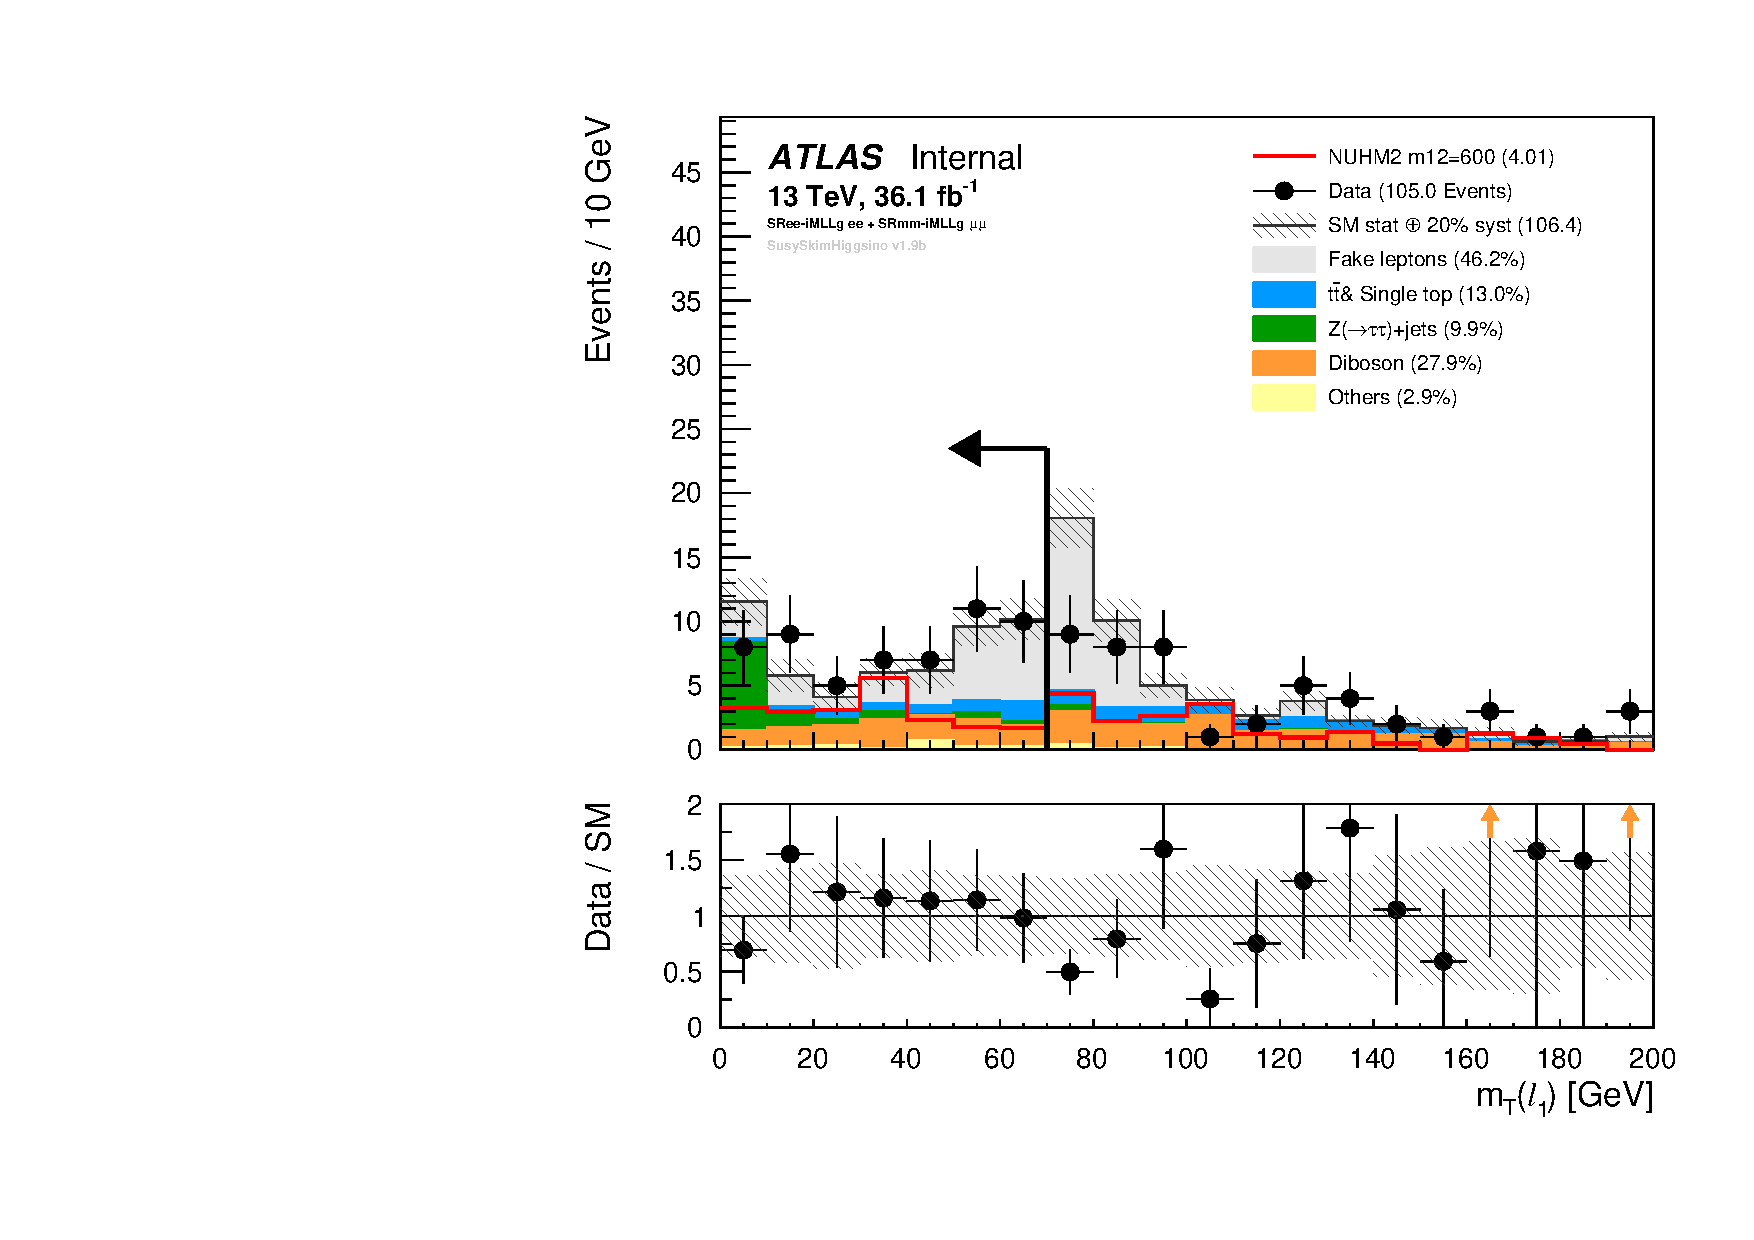
\includegraphics[scale=0.3]{NUHM2_m12_600_and_Bkg_mt_lep1_SFOS_N_minus_one_distribution_in_SR_times_10_on_Nsig.pdf}
            \caption{$m_{T}(\ell_{1})$}
            \label{fig:event_nuhm2_m12_600_mt_lep1_SFOS}
        \end{subfigure}
        \begin{subfigure}[b]{0.48\textwidth}
            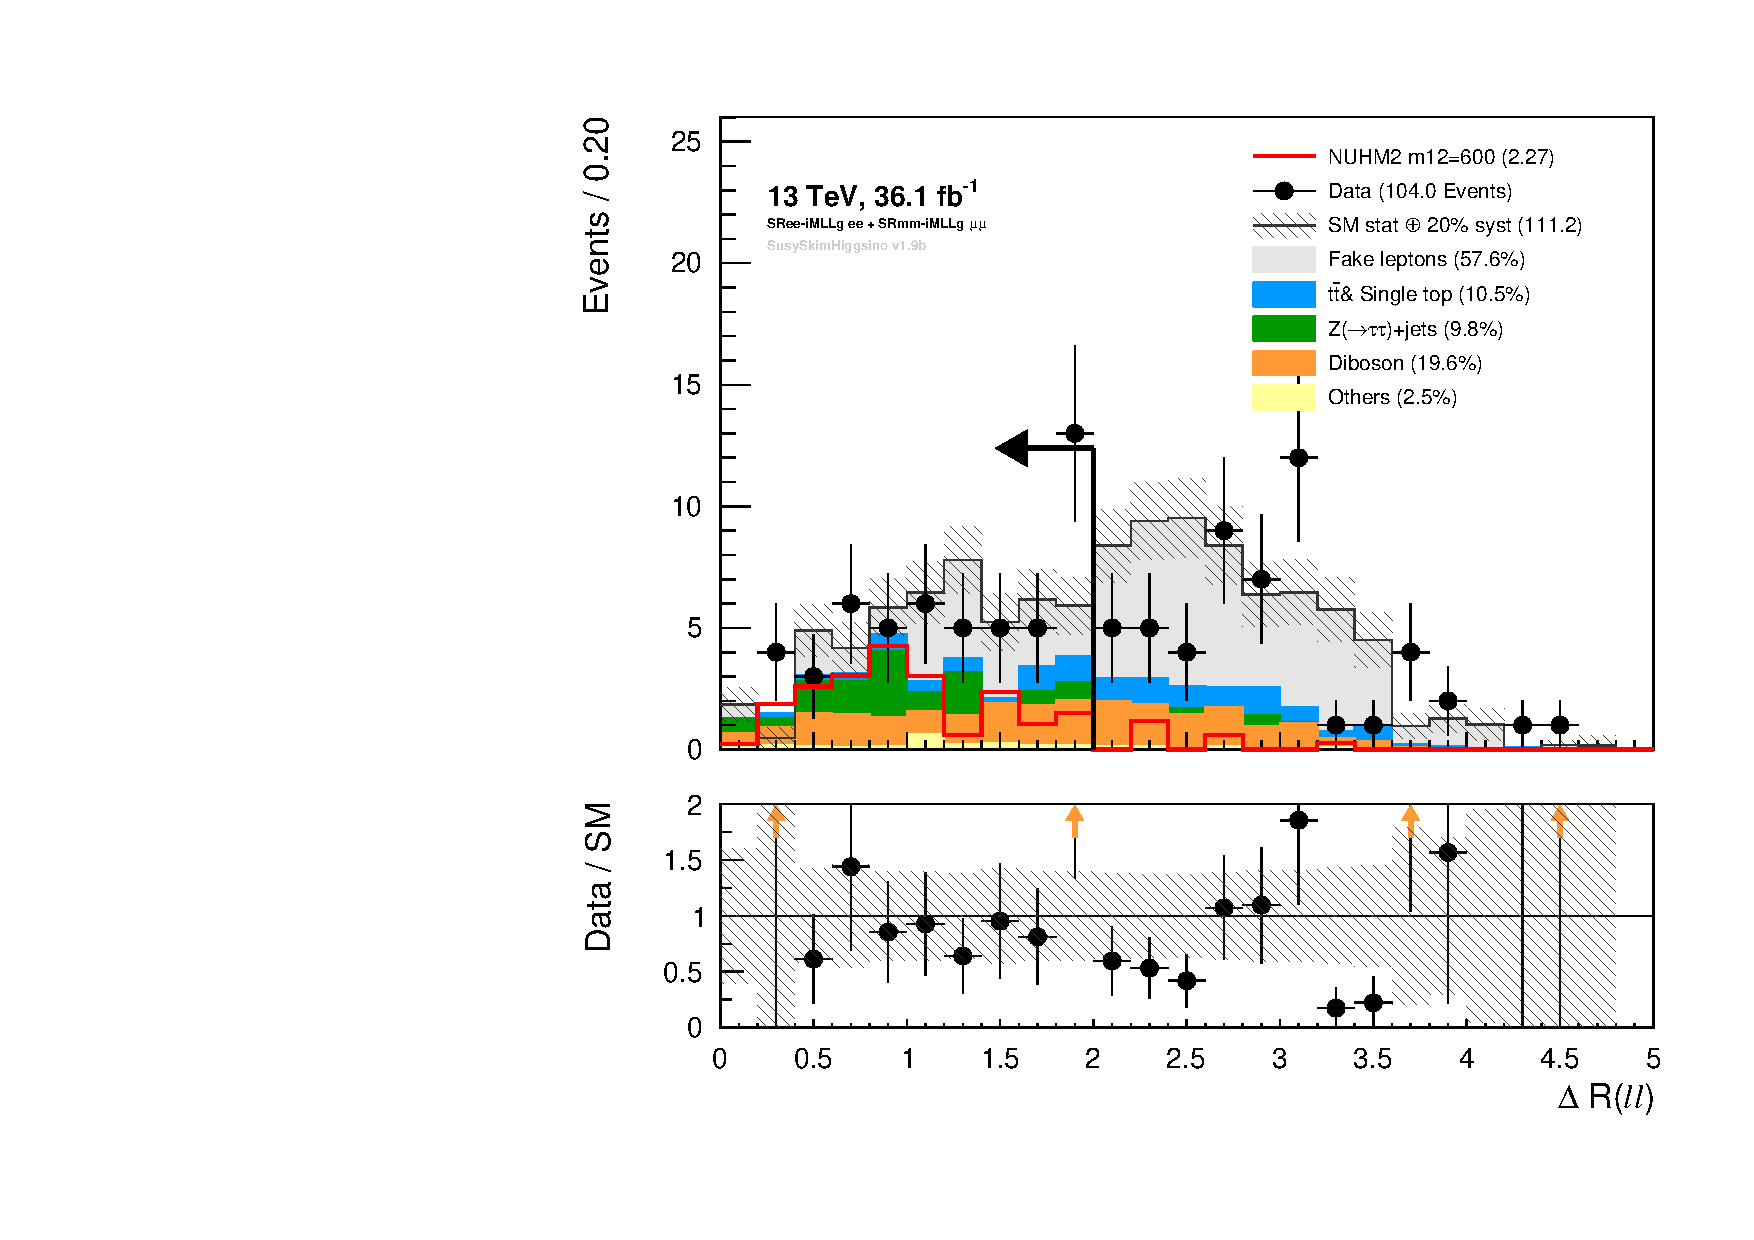
\includegraphics[scale=0.3]{NUHM2_m12_600_and_Bkg_Rll_SFOS_N_minus_one_distribution_in_SR_times_10_on_Nsig.pdf}
            \caption{$\Delta R_{\ell\ell}$}
            \label{fig:event_nuhm2_m12_600_Rll_SFOS}
        \end{subfigure}
        \begin{subfigure}[b]{0.48\textwidth}
            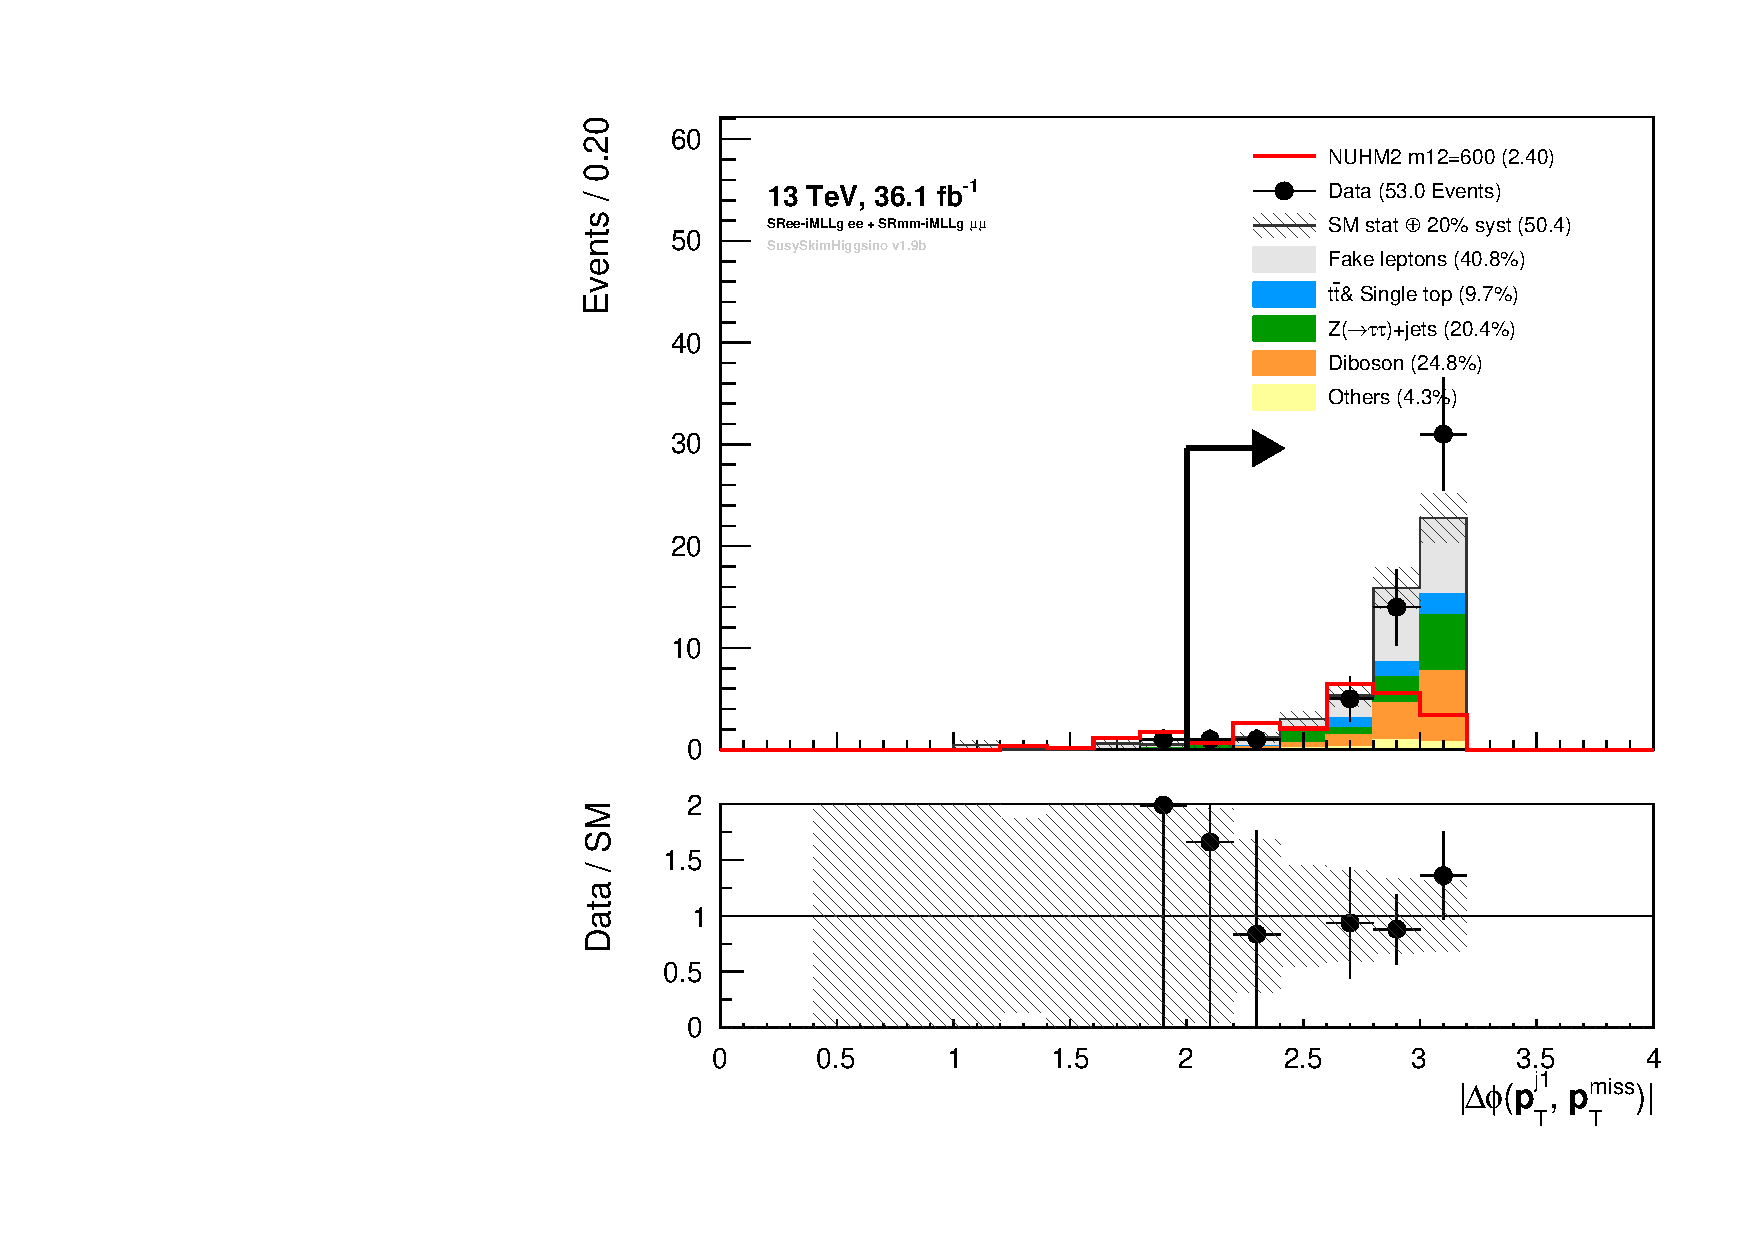
\includegraphics[scale=0.3]{NUHM2_m12_600_and_Bkg_DPhiJ1Met_SFOS_N_minus_one_distribution_in_SR_times_10_on_Nsig.pdf}
            \caption{$|\Delta \phi(\mathbf{p}^{j_{1}}_{\mathrm{T}}, \mathbf{p}^{\mathrm{miss}}_{\mathrm{T}})|$}
            \label{fig:event_nuhm2_m12_600_DPhiJ1Met_SFOS}
        \end{subfigure}
        \begin{subfigure}[b]{0.48\textwidth}
            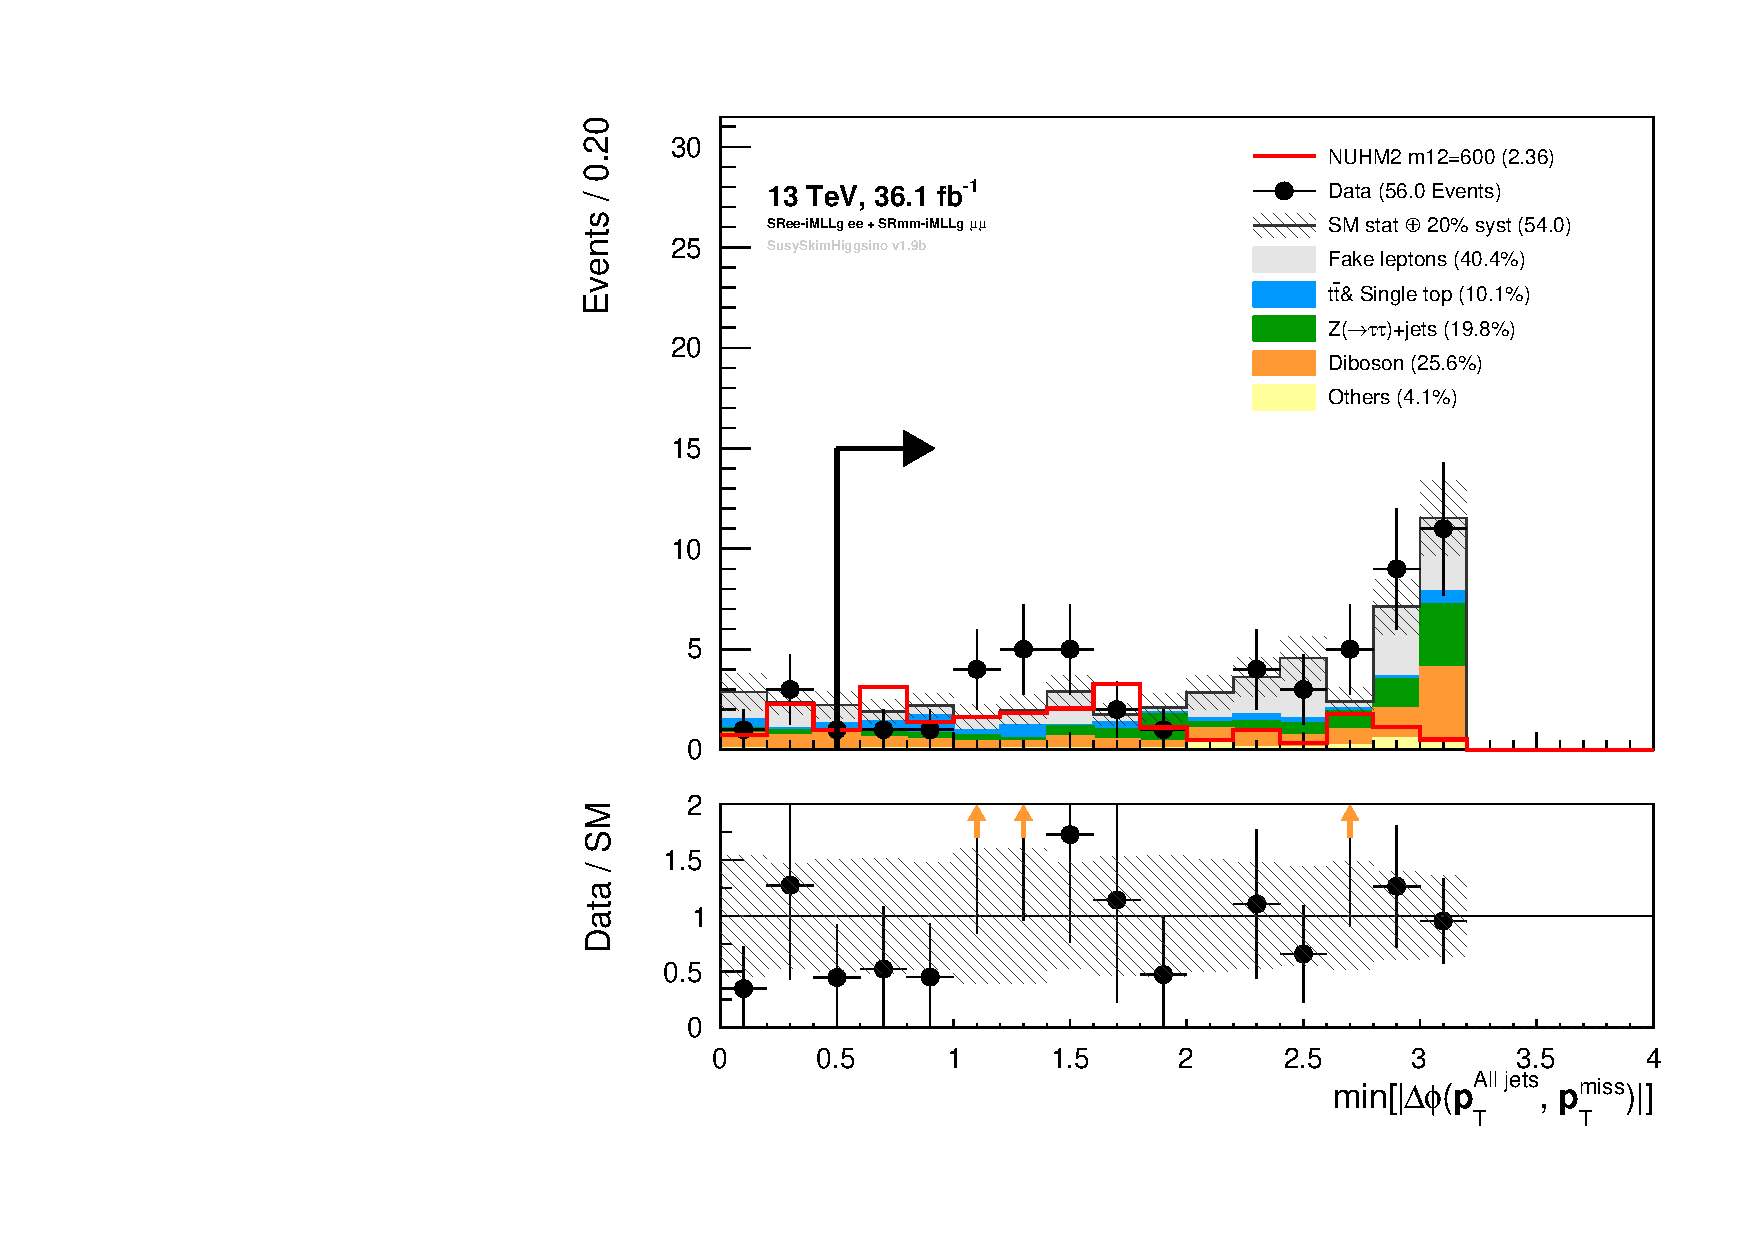
\includegraphics[scale=0.3]{NUHM2_m12_600_and_Bkg_minDPhiAllJetsMet_SFOS_N_minus_one_distribution_in_SR_times_10_on_Nsig.pdf}
            \caption{min[$|\Delta \phi(\mathbf{p}^{\textrm{All jets}}_{\mathrm{T}}, \mathbf{p}^{\mathrm{miss}}_{\mathrm{T}})|$]}
            \label{fig:event_nuhm2_m12_600_minDPhiAllJetsMet_SFOS}
        \end{subfigure}
    \end{center}
    \caption{The `$N-1$' distributions for NUHM2 model with $m_{1/2} = 600$~{\GeV} in SR region $1 < $SR$\ell \ell$-$m_{\ell \ell} < 60$~{\GeV}.
    The NUHM2 distributions are multiplied by 10 but the number of events in the legend use its actual values.}
    \label{fig:dist_nuhm2_kinematic_in_SR_SFOS_m12_600_2}
\end{figure}

% m12 = 700
\begin{figure}[htbp]
    \begin{center}
        \begin{subfigure}[b]{0.48\textwidth}
            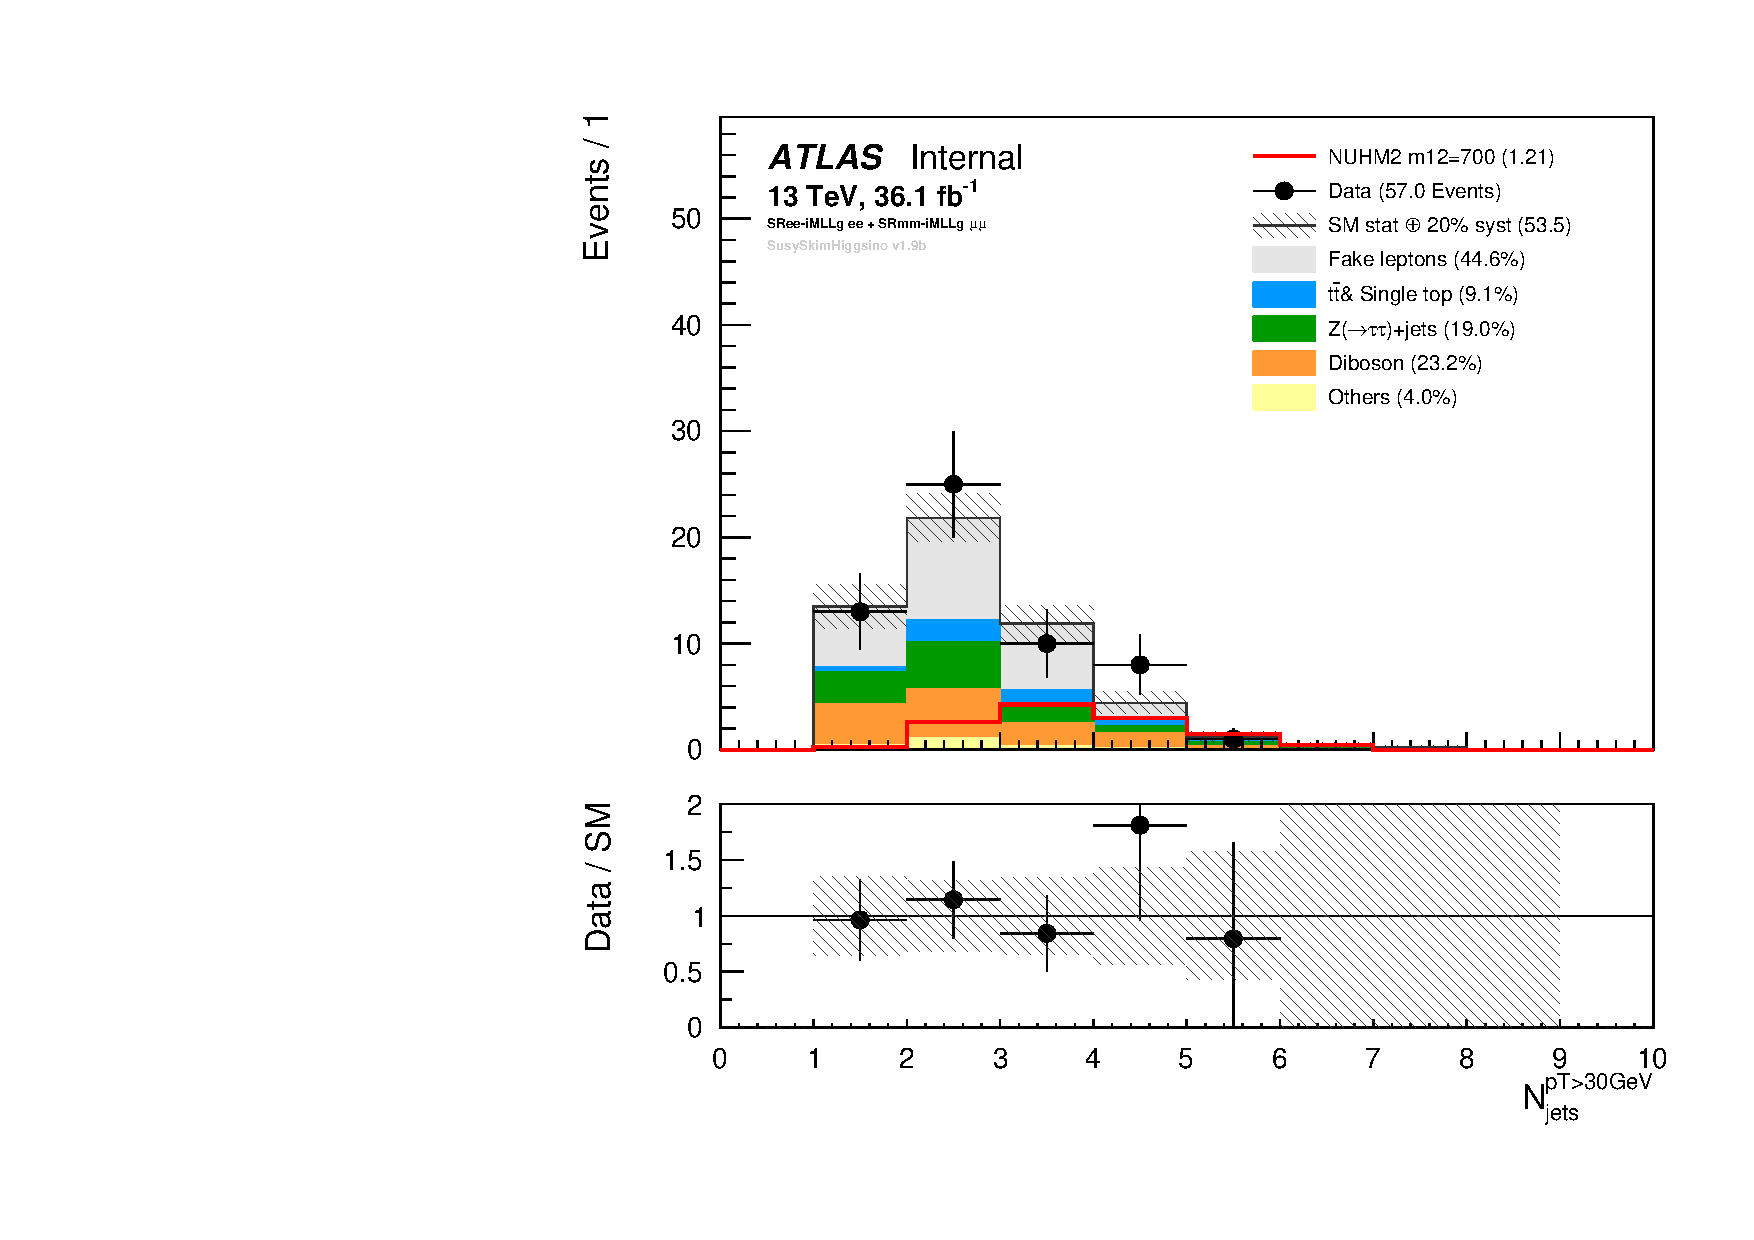
\includegraphics[scale=0.3]{NUHM2_m12_700_and_Bkg_nJet30_SFOS_N_minus_one_distribution_in_SR_times_10_on_Nsig.pdf}
            \caption{$N^{30}_{\mathrm{jets}}$}
            \label{fig:event_nuhm2_m12_700_nJet30_SFOS}
        \end{subfigure}
        \begin{subfigure}[b]{0.48\textwidth}
            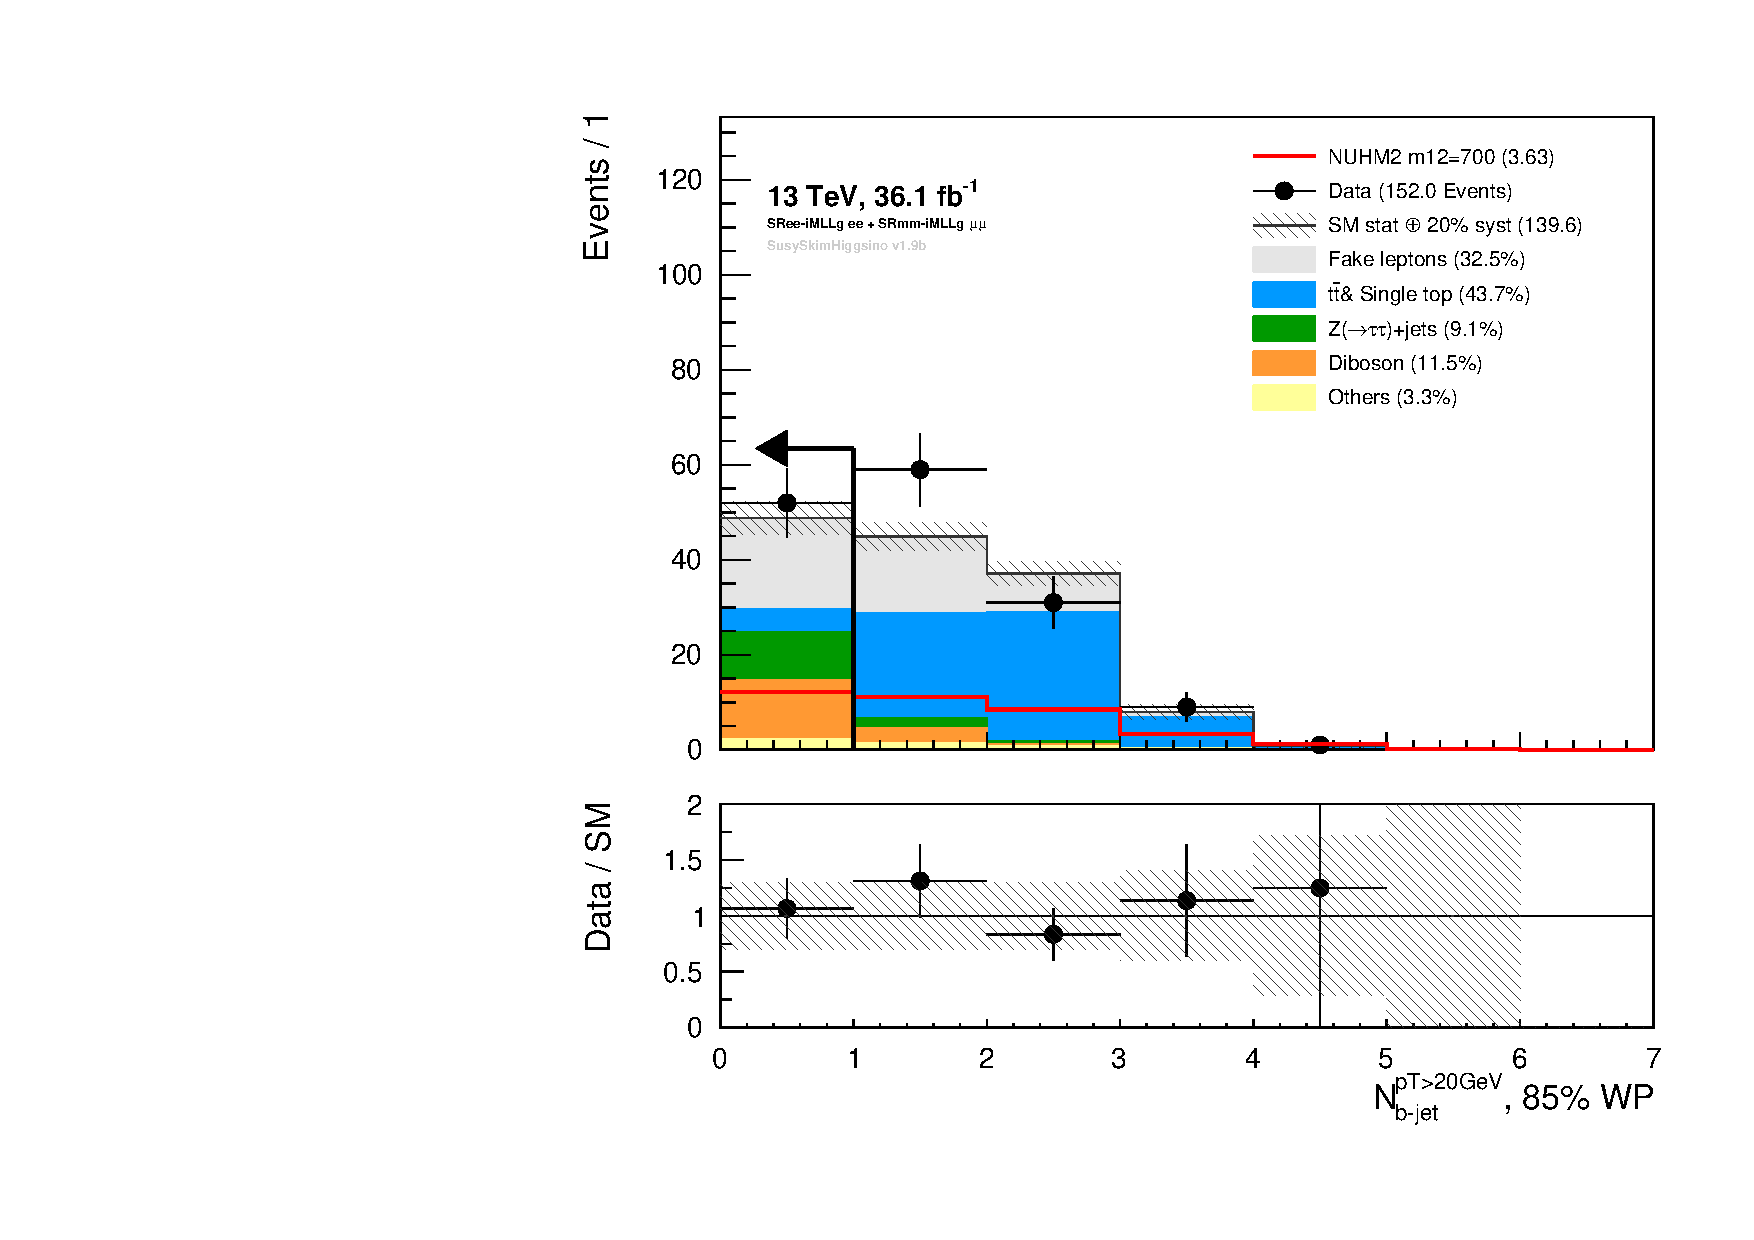
\includegraphics[scale=0.3]{NUHM2_m12_700_and_Bkg_nBJet20_MV2c10_SFOS_N_minus_one_distribution_in_SR_times_10_on_Nsig.pdf}
            \caption{$N^{20}_{\mathrm{b-jets}}$}
            \label{fig:event_nuhm2_m12_700_nBJet20_SFOS}
        \end{subfigure}
        \begin{subfigure}[b]{0.48\textwidth}
            \includegraphics[scale=0.3]{NUHM2_m12_700_and_Bkg_lep1Pt_SFOS_N_minus_one_distribution_in_SR_times_10_on_Nsig.pdf}
            \caption{$p^{\ell_1}_{\mathrm{T}}$}
            \label{fig:event_nuhm2_m12_700_lep1Pt_SFOS}
        \end{subfigure}
        \begin{subfigure}[b]{0.48\textwidth}
            \includegraphics[scale=0.3]{NUHM2_m12_700_and_Bkg_lep2Pt_SFOS_N_minus_one_distribution_in_SR_times_10_on_Nsig.pdf}
            \caption{$p^{\ell_2}_{\mathrm{T}}$}
            \label{fig:event_nuhm2_m12_700_lep2Pt_SFOS}
        \end{subfigure}
        \begin{subfigure}[b]{0.48\textwidth}
            \includegraphics[scale=0.3]{NUHM2_m12_700_and_Bkg_met_Et_SFOS_N_minus_one_distribution_in_SR_times_10_on_Nsig.pdf}
            \caption{$E^{\mathrm{miss}}_{\mathrm{T}}$}
            \label{fig:event_nuhm2_m12_700_met_SFOS}
        \end{subfigure}
        \begin{subfigure}[b]{0.48\textwidth}
            \includegraphics[scale=0.3]{NUHM2_m12_700_and_Bkg_METOverHTLep_SFOS_N_minus_one_distribution_in_SR_times_10_on_Nsig.pdf}
            \caption{$E^{\mathrm{miss}}_{\mathrm{T}} / H^{\mathrm{leptons}}_{\mathrm{T}}$}
            \label{fig:event_nuhm2_m12_700_METOverHTLep_SFOS}
        \end{subfigure}
    \end{center}
    \caption{The `$N-1$' distributions for NUHM2 model with $m_{1/2} = 700$~{\GeV} in SR region $1 < $SR$\ell \ell$-$m_{\ell \ell} < 60$~{\GeV}.
    The NUHM2 distributions are multiplied by 10 but the number of events in the legend use its actual values.}
    \label{fig:dist_nuhm2_kinematic_in_SR_SFOS_m12_700_1}
\end{figure}

\begin{figure}[htbp]
    \begin{center}
        \begin{subfigure}[b]{0.48\textwidth}
            \includegraphics[scale=0.3]{NUHM2_m12_700_and_Bkg_mll_SFOS_N_minus_one_distribution_in_SR_times_10_on_Nsig.pdf}
            \caption{$m_{\ell\ell}$}
            \label{fig:event_nuhm2_m12_700_mll_SFOS}
        \end{subfigure}
        \begin{subfigure}[b]{0.48\textwidth}
            \includegraphics[scale=0.3]{NUHM2_m12_700_and_Bkg_MTauTau_SFOS_N_minus_one_distribution_in_SR_times_10_on_Nsig.pdf}
            \caption{$m_{\tau\tau}$}
            \label{fig:event_nuhm2_m12_700_MTauTau_SFOS}
        \end{subfigure}
        \begin{subfigure}[b]{0.48\textwidth}
            \includegraphics[scale=0.3]{NUHM2_m12_700_and_Bkg_mt_lep1_SFOS_N_minus_one_distribution_in_SR_times_10_on_Nsig.pdf}
            \caption{$m_{T}(\ell_{1})$}
            \label{fig:event_nuhm2_m12_700_mt_lep1_SFOS}
        \end{subfigure}
        \begin{subfigure}[b]{0.48\textwidth}
            \includegraphics[scale=0.3]{NUHM2_m12_700_and_Bkg_Rll_SFOS_N_minus_one_distribution_in_SR_times_10_on_Nsig.pdf}
            \caption{$\Delta R_{\ell\ell}$}
            \label{fig:event_nuhm2_m12_700_Rll_SFOS}
        \end{subfigure}
        \begin{subfigure}[b]{0.48\textwidth}
            \includegraphics[scale=0.3]{NUHM2_m12_700_and_Bkg_DPhiJ1Met_SFOS_N_minus_one_distribution_in_SR_times_10_on_Nsig.pdf}
            \caption{$|\Delta \phi(\mathbf{p}^{j_{1}}_{\mathrm{T}}, \mathbf{p}^{\mathrm{miss}}_{\mathrm{T}})|$}
            \label{fig:event_nuhm2_m12_700_DPhiJ1Met_SFOS}
        \end{subfigure}
        \begin{subfigure}[b]{0.48\textwidth}
            \includegraphics[scale=0.3]{NUHM2_m12_700_and_Bkg_minDPhiAllJetsMet_SFOS_N_minus_one_distribution_in_SR_times_10_on_Nsig.pdf}
            \caption{min[$|\Delta \phi(\mathbf{p}^{\textrm{All jets}}_{\mathrm{T}}, \mathbf{p}^{\mathrm{miss}}_{\mathrm{T}})|$]}
            \label{fig:event_nuhm2_m12_700_minDPhiAllJetsMet_SFOS}
        \end{subfigure}
    \end{center}
    \caption{The `$N-1$' distributions for NUHM2 model with $m_{1/2} = 700$~{\GeV} in SR region $1 < $SR$\ell \ell$-$m_{\ell \ell} < 60$~{\GeV}.
    The NUHM2 distributions are multiplied by 10 but the number of events in the legend use its actual values.}
    \label{fig:dist_nuhm2_kinematic_in_SR_SFOS_m12_700_2}
\end{figure}

% m12 = 800
\begin{figure}[htbp]
    \begin{center}
        \begin{subfigure}[b]{0.48\textwidth}
            \includegraphics[scale=0.3]{NUHM2_m12_800_and_Bkg_nJet30_SFOS_N_minus_one_distribution_in_SR_times_10_on_Nsig.pdf}
            \caption{$N^{30}_{\mathrm{jets}}$}
            \label{fig:event_nuhm2_m12_800_nJet30_SFOS}
        \end{subfigure}
        \begin{subfigure}[b]{0.48\textwidth}
            \includegraphics[scale=0.3]{NUHM2_m12_800_and_Bkg_nBJet20_MV2c10_SFOS_N_minus_one_distribution_in_SR_times_10_on_Nsig.pdf}
            \caption{$N^{20}_{\mathrm{b-jets}}$}
            \label{fig:event_nuhm2_m12_800_nBJet20_SFOS}
        \end{subfigure}
        \begin{subfigure}[b]{0.48\textwidth}
            \includegraphics[scale=0.3]{NUHM2_m12_800_and_Bkg_lep1Pt_SFOS_N_minus_one_distribution_in_SR_times_10_on_Nsig.pdf}
            \caption{$p^{\ell_1}_{\mathrm{T}}$}
            \label{fig:event_nuhm2_m12_800_lep1Pt_SFOS}
        \end{subfigure}
        \begin{subfigure}[b]{0.48\textwidth}
            \includegraphics[scale=0.3]{NUHM2_m12_800_and_Bkg_lep2Pt_SFOS_N_minus_one_distribution_in_SR_times_10_on_Nsig.pdf}
            \caption{$p^{\ell_2}_{\mathrm{T}}$}
            \label{fig:event_nuhm2_m12_800_lep2Pt_SFOS}
        \end{subfigure}
        \begin{subfigure}[b]{0.48\textwidth}
            \includegraphics[scale=0.3]{NUHM2_m12_800_and_Bkg_met_Et_SFOS_N_minus_one_distribution_in_SR_times_10_on_Nsig.pdf}
            \caption{$E^{\mathrm{miss}}_{\mathrm{T}}$}
            \label{fig:event_nuhm2_m12_800_met_SFOS}
        \end{subfigure}
        \begin{subfigure}[b]{0.48\textwidth}
            \includegraphics[scale=0.3]{NUHM2_m12_800_and_Bkg_METOverHTLep_SFOS_N_minus_one_distribution_in_SR_times_10_on_Nsig.pdf}
            \caption{$E^{\mathrm{miss}}_{\mathrm{T}} / H^{\mathrm{leptons}}_{\mathrm{T}}$}
            \label{fig:event_nuhm2_m12_800_METOverHTLep_SFOS}
        \end{subfigure}
    \end{center}
    \caption{The `$N-1$' distributions for NUHM2 model with $m_{1/2} = 800$~{\GeV} in SR region $1 < $SR$\ell \ell$-$m_{\ell \ell} < 60$~{\GeV}.
    The NUHM2 distributions are multiplied by 10 but the number of events in the legend use its actual values.}
    \label{fig:dist_nuhm2_kinematic_in_SR_SFOS_m12_800_1}
\end{figure}

\begin{figure}[htbp]
    \begin{center}
        \begin{subfigure}[b]{0.48\textwidth}
            \includegraphics[scale=0.3]{NUHM2_m12_800_and_Bkg_mll_SFOS_N_minus_one_distribution_in_SR_times_10_on_Nsig.pdf}
            \caption{$m_{\ell\ell}$}
            \label{fig:event_nuhm2_m12_800_mll_SFOS}
        \end{subfigure}
        \begin{subfigure}[b]{0.48\textwidth}
            \includegraphics[scale=0.3]{NUHM2_m12_800_and_Bkg_MTauTau_SFOS_N_minus_one_distribution_in_SR_times_10_on_Nsig.pdf}
            \caption{$m_{\tau\tau}$}
            \label{fig:event_nuhm2_m12_800_MTauTau_SFOS}
        \end{subfigure}
        \begin{subfigure}[b]{0.48\textwidth}
            \includegraphics[scale=0.3]{NUHM2_m12_800_and_Bkg_mt_lep1_SFOS_N_minus_one_distribution_in_SR_times_10_on_Nsig.pdf}
            \caption{$m_{T}(\ell_{1})$}
            \label{fig:event_nuhm2_m12_800_mt_lep1_SFOS}
        \end{subfigure}
        \begin{subfigure}[b]{0.48\textwidth}
            \includegraphics[scale=0.3]{NUHM2_m12_800_and_Bkg_Rll_SFOS_N_minus_one_distribution_in_SR_times_10_on_Nsig.pdf}
            \caption{$\Delta R_{\ell\ell}$}
            \label{fig:event_nuhm2_m12_800_Rll_SFOS}
        \end{subfigure}
        \begin{subfigure}[b]{0.48\textwidth}
            \includegraphics[scale=0.3]{NUHM2_m12_800_and_Bkg_DPhiJ1Met_SFOS_N_minus_one_distribution_in_SR_times_10_on_Nsig.pdf}
            \caption{$|\Delta \phi(\mathbf{p}^{j_{1}}_{\mathrm{T}}, \mathbf{p}^{\mathrm{miss}}_{\mathrm{T}})|$}
            \label{fig:event_nuhm2_m12_800_DPhiJ1Met_SFOS}
        \end{subfigure}
        \begin{subfigure}[b]{0.48\textwidth}
            \includegraphics[scale=0.3]{NUHM2_m12_800_and_Bkg_minDPhiAllJetsMet_SFOS_N_minus_one_distribution_in_SR_times_10_on_Nsig.pdf}
            \caption{min[$|\Delta \phi(\mathbf{p}^{\textrm{All jets}}_{\mathrm{T}}, \mathbf{p}^{\mathrm{miss}}_{\mathrm{T}})|$]}
            \label{fig:event_nuhm2_m12_800_minDPhiAllJetsMet_SFOS}
        \end{subfigure}
    \end{center}
    \caption{The `$N-1$' distributions for NUHM2 model with $m_{1/2} = 800$~{\GeV} in SR region $1 < $SR$\ell \ell$-$m_{\ell \ell} < 60$~{\GeV}.
    The NUHM2 distributions are multiplied by 10 but the number of events in the legend use its actual values.}
    \label{fig:dist_nuhm2_kinematic_in_SR_SFOS_m12_800_2}
\end{figure}

%%%
%%%
%%%

% TRUTH comparison
% m12 = 600
\begin{figure}[htbp]
    \begin{center}
        \begin{subfigure}[b]{0.48\textwidth}
            \includegraphics[scale=0.4]{nBaselineLeptons.pdf}
            \caption{Baseline leptons multiplicities}
        \end{subfigure}
        \begin{subfigure}[b]{0.48\textwidth}
            \includegraphics[scale=0.4]{nSignalLeptons.pdf}
            \caption{Signal leptons multiplicities}
        \end{subfigure}
        \begin{subfigure}[b]{0.48\textwidth}
            \includegraphics[scale=0.4]{nElectrons.pdf}
            \caption{Signal electrons multiplicities}
        \end{subfigure}
        \begin{subfigure}[b]{0.48\textwidth}
            \includegraphics[scale=0.4]{nMuons.pdf}
            \caption{Signal muons multiplicities}
        \end{subfigure}
    \end{center}
    \caption{The lepton multiplicity distributions.
    The lepton multiplicity of NUHM2 with $m_{1/2} = 600$~{\GeV} are compared to the simplified Higgsino model with $m_{\widetilde{\chi}^{0}_{2}}=170$~{\GeV} and $m_{\widetilde{\chi}^{0}_{1}}=150$~{\GeV}.
    Four different production channels, $\widetilde{\chi}^{0}_{2}\widetilde{\chi}^{0}_{1}$, $\widetilde{\chi}^{0}_{2}\widetilde{\chi}^{+}_{1}$, $\widetilde{\chi}^{0}_{2}\widetilde{\chi}^{-}_{1}$, and $\widetilde{\chi}^{\pm}_{1}\widetilde{\chi}^{\mp}_{1}$, for the NUHM2 and the simplified Higgsino model are considered.
    The distributions of four productions are combined and normalized to equal area.}
    \label{fig:dist_nuhm2_lepton_multiplicity}
\end{figure}

\begin{figure}[htbp]
    \begin{center}
        \begin{subfigure}[b]{0.48\textwidth}
            \includegraphics[scale=0.4]{nJets.pdf}
            \caption{Jets multiplicity}
        \end{subfigure}
        \begin{subfigure}[b]{0.48\textwidth}
            \includegraphics[scale=0.4]{nBjets.pdf}
            \caption{$b$-jets multiplicity}
        \end{subfigure}
        \begin{subfigure}[b]{0.48\textwidth}
            \includegraphics[scale=0.4]{nJet25.pdf}
            \caption{Signal jets multiplicity with $\pt > 25$~{\GeV}}
        \end{subfigure}
        \begin{subfigure}[b]{0.48\textwidth}
            \includegraphics[scale=0.4]{nJet30.pdf}
            \caption{Signal jets multiplicity with $\pt > 30$~{\GeV}}
        \end{subfigure}
    \end{center}
    \caption{The jets multiplicity distributions.
    The jet multiplicity of NUHM2 with $m_{1/2} = 600$~{\GeV} are compared to the simplified Higgsino model with $m_{\widetilde{\chi}^{0}_{2}}=170$~{\GeV} and $m_{\widetilde{\chi}^{0}_{1}}=150$~{\GeV}.
    The top left plot includes the forward jets and the bottom two plots use the signal jets with $\pt > 25$~{\GeV} and $\pt > 30$~{\GeV}, respectively.
    Four different production channels, $\widetilde{\chi}^{0}_{2}\widetilde{\chi}^{0}_{1}$, $\widetilde{\chi}^{0}_{2}\widetilde{\chi}^{+}_{1}$, $\widetilde{\chi}^{0}_{2}\widetilde{\chi}^{-}_{1}$, and $\widetilde{\chi}^{\pm}_{1}\widetilde{\chi}^{\mp}_{1}$, for the NUHM2 and the simplified Higgsino model are considered.
    The distributions of four productions are combined and normalized to equal area.}
    \label{fig:dist_nuhm2_jets_multiplicity}
\end{figure}

\begin{figure}[htbp]
    \begin{center}
        \begin{subfigure}[b]{0.48\textwidth}
            \includegraphics[scale=0.35]{signalElectrons_pt.pdf}
            \caption{Signal electrons \pt}
        \end{subfigure}
        \begin{subfigure}[b]{0.48\textwidth}
            \includegraphics[scale=0.35]{signalMuons_pt.pdf}
            \caption{Signal muons \pt}
        \end{subfigure}
        \begin{subfigure}[b]{0.48\textwidth}
            \includegraphics[scale=0.35]{signalElectrons_eta.pdf}
            \caption{Signal electrons $\eta$}
        \end{subfigure}
        \begin{subfigure}[b]{0.48\textwidth}
            \includegraphics[scale=0.35]{signalMuons_eta.pdf}
            \caption{Signal muons $\eta$}
        \end{subfigure}
        \begin{subfigure}[b]{0.48\textwidth}
            \includegraphics[scale=0.35]{signalElectrons_phi.pdf}
            \caption{Signal electrons $\phi$}
        \end{subfigure}
        \begin{subfigure}[b]{0.48\textwidth}
            \includegraphics[scale=0.35]{signalMuons_phi.pdf}
            \caption{Signal muons $\phi$}
        \end{subfigure}
    \end{center}
    \caption{The \pt, $\eta$, and $\phi$ distributions for the NUHM2 with $m_{1/2} = 600$~{\GeV} and the simplified Higgsino model with $m_{\widetilde{\chi}^{0}_{2}}=170$~{\GeV} and $m_{\widetilde{\chi}^{0}_{1}}=150$~{\GeV}.
    The signal electrons \pt, $\eta$, and $\phi$ distributions are on the left column and the signal muons distributions are on the right.
    Four different production channels, $\widetilde{\chi}^{0}_{2}\widetilde{\chi}^{0}_{1}$, $\widetilde{\chi}^{0}_{2}\widetilde{\chi}^{+}_{1}$, $\widetilde{\chi}^{0}_{2}\widetilde{\chi}^{-}_{1}$, and $\widetilde{\chi}^{\pm}_{1}\widetilde{\chi}^{\mp}_{1}$, for the NUHM2 and the simplified Higgsino model are considered.
    The distributions of four productions are combined and normalized to equal area.}
    \label{fig:dist_nuhm2_leptons_pt_eta_phi}
\end{figure}

\begin{figure}[htbp]
    \begin{center}
        \begin{subfigure}[b]{0.48\textwidth}
            \includegraphics[scale=0.35]{signalJets_pt.pdf}
            \caption{The signal jets \pt.}
        \end{subfigure}
        \begin{subfigure}[b]{0.48\textwidth}
            \includegraphics[scale=0.35]{signalBjets_pt.pdf}
            \caption{The signal $b$-jets \pt.}
        \end{subfigure}
        \begin{subfigure}[b]{0.48\textwidth}
            \includegraphics[scale=0.35]{signalJets_eta.pdf}
            \caption{The signal jets $\eta$.}
        \end{subfigure}
        \begin{subfigure}[b]{0.48\textwidth}
            \includegraphics[scale=0.35]{signalBjets_eta.pdf}
            \caption{The signal $b$-jets $\eta$.}
        \end{subfigure}
        \begin{subfigure}[b]{0.48\textwidth}
            \includegraphics[scale=0.35]{signalJets_phi.pdf}
            \caption{The signal jets $\phi$.}
        \end{subfigure}
        \begin{subfigure}[b]{0.48\textwidth}
            \includegraphics[scale=0.35]{signalBjets_phi.pdf}
            \caption{The signal $b$-jets $\phi$.}
        \end{subfigure}
    \end{center}
    \caption{The signal jets and the signal $b$-jets \pt, $\eta$, and $\phi$ distributions for the NUHM2 with $m_{1/2} = 600$~{\GeV} and the simplified Higgsino model with $m_{\widetilde{\chi}^{0}_{2}}=170$~{\GeV} and $m_{\widetilde{\chi}^{0}_{1}}=150$~{\GeV}.
    Four different production channels, $\widetilde{\chi}^{0}_{2}\widetilde{\chi}^{0}_{1}$, $\widetilde{\chi}^{0}_{2}\widetilde{\chi}^{+}_{1}$, $\widetilde{\chi}^{0}_{2}\widetilde{\chi}^{-}_{1}$, and $\widetilde{\chi}^{\pm}_{1}\widetilde{\chi}^{\mp}_{1}$, for the NUHM2 and the simplified Higgsino model are considered.
    The distributions of four productions are combined and normalized to equal area.}
    \label{fig:dist_nuhm2_jets_bjets_pt_eta_phi}
\end{figure}

\begin{figure}[htbp]
    \begin{center}
        \begin{subfigure}[b]{0.48\textwidth}
            \includegraphics[scale=0.4]{mll.pdf}
            \caption{$m_{\ell\ell}$}
        \end{subfigure}
        \begin{subfigure}[b]{0.48\textwidth}
            \includegraphics[scale=0.4]{MTauTau.pdf}
            \caption{$m_{\tau\tau}$}
        \end{subfigure}
        \begin{subfigure}[b]{0.48\textwidth}
            \includegraphics[scale=0.4]{mT.pdf}
            \caption{$m_{T}$}
        \end{subfigure}
        \begin{subfigure}[b]{0.48\textwidth}
            \includegraphics[scale=0.4]{mT2.pdf}
            \caption{$m_{T2}$}
        \end{subfigure}
    \end{center}
    \caption{The invariant mass $m_{\ell\ell}$ and $m_{\tau\tau}$ distributions and the transverse mass $m_\mathrm{T}$ and $m_\mathrm{T2}$ distributions.
    The first two leading baseline leptons are used to calculate the $m_{\ell\ell}$ which contains a hump and a tail region.
    The $\widetilde{\chi}^{0}_{2} \widetilde{\chi}^{0}_{1}$ contributes to the hump only and the tail is contributed by the decay products containing the chargino $\widetilde{\chi}^{\pm}_{1}$.
    The Eq.~(\ref{eq:event_mtautau}) is used to calculate the di-tau invariant mass $m_{\tau\tau}$.
    The first or first two leading signal leptons and \met are used to evaluate the transverse mass $m_\mathrm{T}$ and $m_\mathrm{T2}$, respectively.
    Four different production channels, $\widetilde{\chi}^{0}_{2}\widetilde{\chi}^{0}_{1}$, $\widetilde{\chi}^{0}_{2}\widetilde{\chi}^{+}_{1}$, $\widetilde{\chi}^{0}_{2}\widetilde{\chi}^{-}_{1}$, and $\widetilde{\chi}^{\pm}_{1}\widetilde{\chi}^{\mp}_{1}$, for the NUHM2 and the simplified Higgsino model are considered.
    The distributions of four productions are combined and normalized to equal area.}
    \label{fig:dist_nuhm2_mll_mtautau_mT_mT2}
\end{figure}

\begin{figure}[htbp]
    \begin{center}
        \begin{subfigure}[b]{0.48\textwidth}
            \includegraphics[scale=0.4]{met.pdf}
            \caption{\met}
        \end{subfigure}
        \begin{subfigure}[b]{0.48\textwidth}
            \includegraphics[scale=0.4]{METOverHTLep12.pdf}
            \caption{$\met/H_\mathrm{T}^\mathrm{lepton}$}
        \end{subfigure}
        \begin{subfigure}[b]{0.48\textwidth}
            \includegraphics[scale=0.4]{Rll.pdf}
            \caption{$\Delta R(\ell_{1}, \ell_{2})$}
        \end{subfigure}
        \begin{subfigure}[b]{0.48\textwidth}
            \includegraphics[scale=0.4]{dphiMin1.pdf}
            \caption{$\Delta \phi(\met, j_{1})$}
        \end{subfigure}
    \end{center}
    \caption{The \met, $\met/H_\mathrm{T}^\mathrm{lepton}$, $\Delta R(\ell_{1}, \ell_{2})$, and $\Delta \phi(\met, j_{1})$ distributions.
    The $H_\mathrm{T}^\mathrm{lepton}$ is the scalar sum of the first two leading baseline leptons \pt only.
    The distance $\Delta R(\ell_{1}, \ell_{2})$ is calculated by the first two leading baseline leptons and the $\Delta \phi(\met, j_{1})$ uses \met and first leading signal jet.
    Four different production channels, $\widetilde{\chi}^{0}_{2}\widetilde{\chi}^{0}_{1}$, $\widetilde{\chi}^{0}_{2}\widetilde{\chi}^{+}_{1}$, $\widetilde{\chi}^{0}_{2}\widetilde{\chi}^{-}_{1}$, and $\widetilde{\chi}^{\pm}_{1}\widetilde{\chi}^{\mp}_{1}$, for the NUHM2 and the simplified Higgsino model are considered.
    The distributions of four productions are combined and normalized to equal area.}
    \label{fig:dist_nuhm2_met_METOverHTLep12_Rll_dphiMin1}
\end{figure}


%%%
%%%
%%%

% mll reweighting
% m12 = 350
\begin{figure}[htbp]
    \begin{center}
        \begin{subfigure}[b]{0.48\textwidth}
            \includegraphics[scale=0.4]{reweight_Higgsino_160_100_m12_350_nSignalLeptons.pdf}
            \caption{Signal lepton multiplicity}
        \end{subfigure}
        \begin{subfigure}[b]{0.48\textwidth}
            \includegraphics[scale=0.4]{reweight_Higgsino_160_100_m12_350_signalLeptons_pt.pdf}
            \caption{Signal lepton \pt}
        \end{subfigure}
        \begin{subfigure}[b]{0.48\textwidth}
            \includegraphics[scale=0.4]{reweight_Higgsino_160_100_m12_350_pTLep1.pdf}
            \caption{Leading lepton \pt}
        \end{subfigure}
        \begin{subfigure}[b]{0.48\textwidth}
            \includegraphics[scale=0.4]{reweight_Higgsino_160_100_m12_350_pTLep2.pdf}
            \caption{Subleading lepton \pt}
        \end{subfigure}
    \end{center}
    \caption{The distributions for signal lepton multiplicity, all signal leptons \pt, the leading lepton \pt, and the subleading lepton \pt.
    The NUHM2 signal sample uses  $m_{1/2} = 350$~{\GeV} and the Higgsino signal sample uses $m_{\widetilde{\chi}^{0}_{2}} = 160$ and $m_{\widetilde{\chi}^{0}_{1}} = 100$~{\GeV}.
    The reweighted Higgsino sample is shown in red line.
    The lower pad shows the ratio between NUHM2 and Higgsino (or reweighted Higgsino) distributions.}
    \label{fig:dist_nuhm2_reweighting_validation_m12_350_1}
\end{figure}

\begin{figure}[htbp]
    \begin{center}
        \begin{subfigure}[b]{0.48\textwidth}
            \includegraphics[scale=0.4]{reweight_Higgsino_160_100_m12_350_nJets.pdf}
            \caption{Jet multiplicity}
        \end{subfigure}
        \begin{subfigure}[b]{0.48\textwidth}
            \includegraphics[scale=0.4]{reweight_Higgsino_160_100_m12_350_signalJets_pt.pdf}
            \caption{Jet \pt}
        \end{subfigure}
        \begin{subfigure}[b]{0.48\textwidth}
            \includegraphics[scale=0.4]{reweight_Higgsino_160_100_m12_350_nBjets.pdf}
            \caption{$b$-jets multiplicity}
        \end{subfigure}
        \begin{subfigure}[b]{0.48\textwidth}
            \includegraphics[scale=0.4]{reweight_Higgsino_160_100_m12_350_signalBjets_pt.pdf}
            \caption{$b$-jets \pt}
        \end{subfigure}
    \end{center}
    \caption{The distributions for jet multiplicity, jet \pt, $b$-jets multiplicity, and $b$-jet \pt.
    The NUHM2 signal sample uses  $m_{1/2} = 350$~{\GeV} and the Higgsino signal sample uses $m_{\widetilde{\chi}^{0}_{2}} = 160$ and $m_{\widetilde{\chi}^{0}_{1}} = 100$~{\GeV}.
    The reweighted Higgsino sample is shown in red line.
    The lower pad shows the ratio between NUHM2 and Higgsino (or reweighted Higgsino) distributions.}
    \label{fig:dist_nuhm2_reweighting_validation_m12_350_2}
\end{figure}

\begin{figure}[htbp]
    \begin{center}
        \begin{subfigure}[b]{0.48\textwidth}
            \includegraphics[scale=0.4]{reweight_Higgsino_160_100_m12_350_met.pdf}
            \caption{\met}
        \end{subfigure}
        \begin{subfigure}[b]{0.48\textwidth}
            \includegraphics[scale=0.4]{reweight_Higgsino_160_100_m12_350_METOverHTLep12.pdf}
            \caption{$\met/H^\mathrm{leptons}_\mathrm{T}$}
        \end{subfigure}
        \begin{subfigure}[b]{0.48\textwidth}
            \includegraphics[scale=0.4]{reweight_Higgsino_160_100_m12_350_mll.pdf}
            \caption{$m_{\ell \ell}$}
        \end{subfigure}
        \begin{subfigure}[b]{0.48\textwidth}
            \includegraphics[scale=0.4]{reweight_Higgsino_160_100_m12_350_MTauTau.pdf}
            \caption{$m_{\tau \tau}$}
        \end{subfigure}
    \end{center}
    \caption{The distributions for \met, $\met/H^\mathrm{leptons}_\mathrm{T}$, $m_{\ell \ell}$, and $m_{\tau \tau}$.
    The NUHM2 signal sample uses  $m_{1/2} = 350$~{\GeV} and the Higgsino signal sample uses $m_{\widetilde{\chi}^{0}_{2}} = 160$ and $m_{\widetilde{\chi}^{0}_{1}} = 100$~{\GeV}.
    The reweighted Higgsino sample is shown in red line.
    The lower pad shows the ratio between NUHM2 and Higgsino (or reweighted Higgsino) distributions.}
    \label{fig:dist_nuhm2_reweighting_validation_m12_350_3}
\end{figure}

\begin{figure}[htbp]
    \begin{center}
        \begin{subfigure}[b]{0.48\textwidth}
            \includegraphics[scale=0.4]{reweight_Higgsino_160_100_m12_350_mT.pdf}
            \caption{$m_\mathrm{T}$}
        \end{subfigure}
        \begin{subfigure}[b]{0.48\textwidth}
            \includegraphics[scale=0.4]{reweight_Higgsino_160_100_m12_350_mT2.pdf}
            \caption{$m_\mathrm{T2}$}
        \end{subfigure}
        \begin{subfigure}[b]{0.48\textwidth}
            \includegraphics[scale=0.4]{reweight_Higgsino_160_100_m12_350_meffIncl.pdf}
            \caption{$m^\mathrm{Incl}_\mathrm{eff}$}
        \end{subfigure}
        \begin{subfigure}[b]{0.48\textwidth}
            \includegraphics[scale=0.4]{reweight_Higgsino_160_100_m12_350_HTIncl.pdf}
            \caption{$H^\mathrm{Incl}_\mathrm{T}$}
        \end{subfigure}
    \end{center}
    \caption{The distributions for $m_\mathrm{T}$, $m_\mathrm{T2}$, $m^\mathrm{Incl}_\mathrm{eff}$, $H^\mathrm{Incl}_\mathrm{T}$.
    The NUHM2 signal sample uses  $m_{1/2} = 350$~{\GeV} and the Higgsino signal sample uses $m_{\widetilde{\chi}^{0}_{2}} = 160$ and $m_{\widetilde{\chi}^{0}_{1}} = 100$~{\GeV}.
    The reweighted Higgsino sample is shown in red line.
    The lower pad shows the ratio between NUHM2 and Higgsino (or reweighted Higgsino) distributions.}
    \label{fig:dist_nuhm2_reweighting_validation_m12_350_4}
\end{figure}

\begin{figure}[htbp]
    \begin{center}
        \begin{subfigure}[b]{0.48\textwidth}
            \includegraphics[scale=0.4]{reweight_Higgsino_160_100_m12_350_Rll.pdf}
            \caption{$\Delta R_{\ell \ell}$}
        \end{subfigure}
        \begin{subfigure}[b]{0.48\textwidth}
            \includegraphics[scale=0.4]{reweight_Higgsino_160_100_m12_350_dphiMin1.pdf}
            \caption{$\Delta \phi(\mathbf{p}^\mathrm{j1}_\mathrm{T}, \mathbf{p}^\mathrm{miss}_\mathrm{T})$}
        \end{subfigure}
    \end{center}
    \caption{The distributions for $\Delta R_{\ell \ell}$ and $\Delta \phi(\mathbf{p}^\mathrm{j1}_\mathrm{T}, \mathbf{p}^\mathrm{miss}_\mathrm{T})$.
    The NUHM2 signal sample uses  $m_{1/2} = 350$~{\GeV} and the Higgsino signal sample uses $m_{\widetilde{\chi}^{0}_{2}} = 160$ and $m_{\widetilde{\chi}^{0}_{1}} = 100$~{\GeV}.
    The reweighted Higgsino sample is shown in red line.
    The lower pad shows the ratio between NUHM2 and Higgsino (or reweighted Higgsino) distributions.}
    \label{fig:dist_nuhm2_reweighting_validation_m12_350_5}
\end{figure}

% m12 = 400
\begin{figure}[htbp]
    \begin{center}
        \begin{subfigure}[b]{0.48\textwidth}
            \includegraphics[scale=0.4]{reweight_Higgsino_190_150_m12_400_nSignalLeptons.pdf}
            \caption{Signal lepton multiplicity}
        \end{subfigure}
        \begin{subfigure}[b]{0.48\textwidth}
            \includegraphics[scale=0.4]{reweight_Higgsino_190_150_m12_400_signalLeptons_pt.pdf}
            \caption{Signal lepton \pt}
        \end{subfigure}
        \begin{subfigure}[b]{0.48\textwidth}
            \includegraphics[scale=0.4]{reweight_Higgsino_190_150_m12_400_pTLep1.pdf}
            \caption{Leading lepton \pt}
        \end{subfigure}
        \begin{subfigure}[b]{0.48\textwidth}
            \includegraphics[scale=0.4]{reweight_Higgsino_190_150_m12_400_pTLep2.pdf}
            \caption{Subleading lepton \pt}
        \end{subfigure}
    \end{center}
    \caption{The distributions for signal lepton multiplicity, all signal leptons \pt, the leading lepton \pt, and the subleading lepton \pt.
    The NUHM2 signal sample uses  $m_{1/2} = 400$~{\GeV} and the Higgsino signal sample uses $m_{\widetilde{\chi}^{0}_{2}} = 190$ and $m_{\widetilde{\chi}^{0}_{1}} = 150$~{\GeV}.
    The reweighted Higgsino sample is shown in red line.
    The lower pad shows the ratio between NUHM2 and Higgsino (or reweighted Higgsino) distributions.}
    \label{fig:dist_nuhm2_reweighting_validation_m12_400_1}
\end{figure}

\begin{figure}[htbp]
    \begin{center}
        \begin{subfigure}[b]{0.48\textwidth}
            \includegraphics[scale=0.4]{reweight_Higgsino_190_150_m12_400_nJets.pdf}
            \caption{Jet multiplicity}
        \end{subfigure}
        \begin{subfigure}[b]{0.48\textwidth}
            \includegraphics[scale=0.4]{reweight_Higgsino_190_150_m12_400_signalJets_pt.pdf}
            \caption{Jet \pt}
        \end{subfigure}
        \begin{subfigure}[b]{0.48\textwidth}
            \includegraphics[scale=0.4]{reweight_Higgsino_190_150_m12_400_nBjets.pdf}
            \caption{$b$-jets multiplicity}
        \end{subfigure}
        \begin{subfigure}[b]{0.48\textwidth}
            \includegraphics[scale=0.4]{reweight_Higgsino_190_150_m12_400_signalBjets_pt.pdf}
            \caption{$b$-jets \pt}
        \end{subfigure}
    \end{center}
    \caption{The distributions for jet multiplicity, jet \pt, $b$-jets multiplicity, and $b$-jet \pt.
    The NUHM2 signal sample uses  $m_{1/2} = 400$~{\GeV} and the Higgsino signal sample uses $m_{\widetilde{\chi}^{0}_{2}} = 190$ and $m_{\widetilde{\chi}^{0}_{1}} = 150$~{\GeV}.
    The reweighted Higgsino sample is shown in red line.
    The lower pad shows the ratio between NUHM2 and Higgsino (or reweighted Higgsino) distributions.}
    \label{fig:dist_nuhm2_reweighting_validation_m12_400_2}
\end{figure}

\begin{figure}[htbp]
    \begin{center}
        \begin{subfigure}[b]{0.48\textwidth}
            \includegraphics[scale=0.4]{reweight_Higgsino_190_150_m12_400_met.pdf}
            \caption{\met}
        \end{subfigure}
        \begin{subfigure}[b]{0.48\textwidth}
            \includegraphics[scale=0.4]{reweight_Higgsino_190_150_m12_400_METOverHTLep12.pdf}
            \caption{$\met/H^\mathrm{leptons}_\mathrm{T}$}
        \end{subfigure}
        \begin{subfigure}[b]{0.48\textwidth}
            \includegraphics[scale=0.4]{reweight_Higgsino_190_150_m12_400_mll.pdf}
            \caption{$m_{\ell \ell}$}
        \end{subfigure}
        \begin{subfigure}[b]{0.48\textwidth}
            \includegraphics[scale=0.4]{reweight_Higgsino_190_150_m12_400_MTauTau.pdf}
            \caption{$m_{\tau \tau}$}
        \end{subfigure}
    \end{center}
    \caption{The distributions for \met, $\met/H^\mathrm{leptons}_\mathrm{T}$, $m_{\ell \ell}$, and $m_{\tau \tau}$.
    The NUHM2 signal sample uses  $m_{1/2} = 400$~{\GeV} and the Higgsino signal sample uses $m_{\widetilde{\chi}^{0}_{2}} = 190$ and $m_{\widetilde{\chi}^{0}_{1}} = 150$~{\GeV}.
    The reweighted Higgsino sample is shown in red line.
    The lower pad shows the ratio between NUHM2 and Higgsino (or reweighted Higgsino) distributions.}
    \label{fig:dist_nuhm2_reweighting_validation_m12_400_3}
\end{figure}

\begin{figure}[htbp]
    \begin{center}
        \begin{subfigure}[b]{0.48\textwidth}
            \includegraphics[scale=0.4]{reweight_Higgsino_190_150_m12_400_mT.pdf}
            \caption{$m_\mathrm{T}$}
        \end{subfigure}
        \begin{subfigure}[b]{0.48\textwidth}
            \includegraphics[scale=0.4]{reweight_Higgsino_190_150_m12_400_mT2.pdf}
            \caption{$m_\mathrm{T2}$}
        \end{subfigure}
        \begin{subfigure}[b]{0.48\textwidth}
            \includegraphics[scale=0.4]{reweight_Higgsino_190_150_m12_400_meffIncl.pdf}
            \caption{$m^\mathrm{Incl}_\mathrm{eff}$}
        \end{subfigure}
        \begin{subfigure}[b]{0.48\textwidth}
            \includegraphics[scale=0.4]{reweight_Higgsino_190_150_m12_400_HTIncl.pdf}
            \caption{$H^\mathrm{Incl}_\mathrm{T}$}
        \end{subfigure}
    \end{center}
    \caption{The distributions for $m_\mathrm{T}$, $m_\mathrm{T2}$, $m^\mathrm{Incl}_\mathrm{eff}$, $H^\mathrm{Incl}_\mathrm{T}$.
    The NUHM2 signal sample uses  $m_{1/2} = 400$~{\GeV} and the Higgsino signal sample uses $m_{\widetilde{\chi}^{0}_{2}} = 190$ and $m_{\widetilde{\chi}^{0}_{1}} = 150$~{\GeV}.
    The reweighted Higgsino sample is shown in red line.
    The lower pad shows the ratio between NUHM2 and Higgsino (or reweighted Higgsino) distributions.}
    \label{fig:dist_nuhm2_reweighting_validation_m12_400_4}
\end{figure}

\begin{figure}[htbp]
    \begin{center}
        \begin{subfigure}[b]{0.48\textwidth}
            \includegraphics[scale=0.4]{reweight_Higgsino_190_150_m12_400_Rll.pdf}
            \caption{$\Delta R_{\ell \ell}$}
        \end{subfigure}
        \begin{subfigure}[b]{0.48\textwidth}
            \includegraphics[scale=0.4]{reweight_Higgsino_190_150_m12_400_dphiMin1.pdf}
            \caption{$\Delta \phi(\mathbf{p}^\mathrm{j1}_\mathrm{T}, \mathbf{p}^\mathrm{miss}_\mathrm{T})$}
        \end{subfigure}
    \end{center}
    \caption{The distributions for $\Delta R_{\ell \ell}$ and $\Delta \phi(\mathbf{p}^\mathrm{j1}_\mathrm{T}, \mathbf{p}^\mathrm{miss}_\mathrm{T})$.
    The NUHM2 signal sample uses  $m_{1/2} = 400$~{\GeV} and the Higgsino signal sample uses $m_{\widetilde{\chi}^{0}_{2}} = 190$ and $m_{\widetilde{\chi}^{0}_{1}} = 150$~{\GeV}.
    The reweighted Higgsino sample is shown in red line.
    The lower pad shows the ratio between NUHM2 and Higgsino (or reweighted Higgsino) distributions.}
    \label{fig:dist_nuhm2_reweighting_validation_m12_400_5}
\end{figure}

% m12 = 500
\begin{figure}[htbp]
    \begin{center}
        \begin{subfigure}[b]{0.48\textwidth}
            \includegraphics[scale=0.4]{reweight_Higgsino_190_150_m12_500_nSignalLeptons.pdf}
            \caption{Signal lepton multiplicity}
        \end{subfigure}
        \begin{subfigure}[b]{0.48\textwidth}
            \includegraphics[scale=0.4]{reweight_Higgsino_190_150_m12_500_signalLeptons_pt.pdf}
            \caption{Signal lepton \pt}
        \end{subfigure}
        \begin{subfigure}[b]{0.48\textwidth}
            \includegraphics[scale=0.4]{reweight_Higgsino_190_150_m12_500_pTLep1.pdf}
            \caption{Leading lepton \pt}
        \end{subfigure}
        \begin{subfigure}[b]{0.48\textwidth}
            \includegraphics[scale=0.4]{reweight_Higgsino_190_150_m12_500_pTLep2.pdf}
            \caption{Subleading lepton \pt}
        \end{subfigure}
    \end{center}
    \caption{The distributions for signal lepton multiplicity, all signal leptons \pt, the leading lepton \pt, and the subleading lepton \pt.
    The NUHM2 signal sample uses  $m_{1/2} = 500$~{\GeV} and the Higgsino signal sample uses $m_{\widetilde{\chi}^{0}_{2}} = 190$ and $m_{\widetilde{\chi}^{0}_{1}} = 150$~{\GeV}.
    The reweighted Higgsino sample is shown in red line.
    The lower pad shows the ratio between NUHM2 and Higgsino (or reweighted Higgsino) distributions.}
    \label{fig:dist_nuhm2_reweighting_validation_m12_500_1}
\end{figure}

\begin{figure}[htbp]
    \begin{center}
        \begin{subfigure}[b]{0.48\textwidth}
            \includegraphics[scale=0.4]{reweight_Higgsino_190_150_m12_500_nJets.pdf}
            \caption{Jet multiplicity}
        \end{subfigure}
        \begin{subfigure}[b]{0.48\textwidth}
            \includegraphics[scale=0.4]{reweight_Higgsino_190_150_m12_500_signalJets_pt.pdf}
            \caption{Jet \pt}
        \end{subfigure}
        \begin{subfigure}[b]{0.48\textwidth}
            \includegraphics[scale=0.4]{reweight_Higgsino_190_150_m12_500_nBjets.pdf}
            \caption{$b$-jets multiplicity}
        \end{subfigure}
        \begin{subfigure}[b]{0.48\textwidth}
            \includegraphics[scale=0.4]{reweight_Higgsino_190_150_m12_500_signalBjets_pt.pdf}
            \caption{$b$-jets \pt}
        \end{subfigure}
    \end{center}
    \caption{The distributions for jet multiplicity, jet \pt, $b$-jets multiplicity, and $b$-jet \pt.
    The NUHM2 signal sample uses  $m_{1/2} = 500$~{\GeV} and the Higgsino signal sample uses $m_{\widetilde{\chi}^{0}_{2}} = 190$ and $m_{\widetilde{\chi}^{0}_{1}} = 150$~{\GeV}.
    The reweighted Higgsino sample is shown in red line.
    The lower pad shows the ratio between NUHM2 and Higgsino (or reweighted Higgsino) distributions.}
    \label{fig:dist_nuhm2_reweighting_validation_m12_500_2}
\end{figure}

\begin{figure}[htbp]
    \begin{center}
        \begin{subfigure}[b]{0.48\textwidth}
            \includegraphics[scale=0.4]{reweight_Higgsino_190_150_m12_500_met.pdf}
            \caption{\met}
        \end{subfigure}
        \begin{subfigure}[b]{0.48\textwidth}
            \includegraphics[scale=0.4]{reweight_Higgsino_190_150_m12_500_METOverHTLep12.pdf}
            \caption{$\met/H^\mathrm{leptons}_\mathrm{T}$}
        \end{subfigure}
        \begin{subfigure}[b]{0.48\textwidth}
            \includegraphics[scale=0.4]{reweight_Higgsino_190_150_m12_500_mll.pdf}
            \caption{$m_{\ell \ell}$}
        \end{subfigure}
        \begin{subfigure}[b]{0.48\textwidth}
            \includegraphics[scale=0.4]{reweight_Higgsino_190_150_m12_500_MTauTau.pdf}
            \caption{$m_{\tau \tau}$}
        \end{subfigure}
    \end{center}
    \caption{The distributions for \met, $\met/H^\mathrm{leptons}_\mathrm{T}$, $m_{\ell \ell}$, and $m_{\tau \tau}$.
    The NUHM2 signal sample uses  $m_{1/2} = 500$~{\GeV} and the Higgsino signal sample uses $m_{\widetilde{\chi}^{0}_{2}} = 190$ and $m_{\widetilde{\chi}^{0}_{1}} = 150$~{\GeV}.
    The reweighted Higgsino sample is shown in red line.
    The lower pad shows the ratio between NUHM2 and Higgsino (or reweighted Higgsino) distributions.}
    \label{fig:dist_nuhm2_reweighting_validation_m12_500_3}
\end{figure}

\begin{figure}[htbp]
    \begin{center}
        \begin{subfigure}[b]{0.48\textwidth}
            \includegraphics[scale=0.4]{reweight_Higgsino_190_150_m12_500_mT.pdf}
            \caption{$m_\mathrm{T}$}
        \end{subfigure}
        \begin{subfigure}[b]{0.48\textwidth}
            \includegraphics[scale=0.4]{reweight_Higgsino_190_150_m12_500_mT2.pdf}
            \caption{$m_\mathrm{T2}$}
        \end{subfigure}
        \begin{subfigure}[b]{0.48\textwidth}
            \includegraphics[scale=0.4]{reweight_Higgsino_190_150_m12_500_meffIncl.pdf}
            \caption{$m^\mathrm{Incl}_\mathrm{eff}$}
        \end{subfigure}
        \begin{subfigure}[b]{0.48\textwidth}
            \includegraphics[scale=0.4]{reweight_Higgsino_190_150_m12_500_HTIncl.pdf}
            \caption{$H^\mathrm{Incl}_\mathrm{T}$}
        \end{subfigure}
    \end{center}
    \caption{The distributions for $m_\mathrm{T}$, $m_\mathrm{T2}$, $m^\mathrm{Incl}_\mathrm{eff}$, $H^\mathrm{Incl}_\mathrm{T}$.
    The NUHM2 signal sample uses  $m_{1/2} = 500$~{\GeV} and the Higgsino signal sample uses $m_{\widetilde{\chi}^{0}_{2}} = 190$ and $m_{\widetilde{\chi}^{0}_{1}} = 150$~{\GeV}.
    The reweighted Higgsino sample is shown in red line.
    The lower pad shows the ratio between NUHM2 and Higgsino (or reweighted Higgsino) distributions.}
    \label{fig:dist_nuhm2_reweighting_validation_m12_500_4}
\end{figure}

\begin{figure}[htbp]
    \begin{center}
        \begin{subfigure}[b]{0.48\textwidth}
            \includegraphics[scale=0.4]{reweight_Higgsino_190_150_m12_500_Rll.pdf}
            \caption{$\Delta R_{\ell \ell}$}
        \end{subfigure}
        \begin{subfigure}[b]{0.48\textwidth}
            \includegraphics[scale=0.4]{reweight_Higgsino_190_150_m12_500_dphiMin1.pdf}
            \caption{$\Delta \phi(\mathbf{p}^\mathrm{j1}_\mathrm{T}, \mathbf{p}^\mathrm{miss}_\mathrm{T})$}
        \end{subfigure}
    \end{center}
    \caption{The distributions for $\Delta R_{\ell \ell}$ and $\Delta \phi(\mathbf{p}^\mathrm{j1}_\mathrm{T}, \mathbf{p}^\mathrm{miss}_\mathrm{T})$.
    The NUHM2 signal sample uses  $m_{1/2} = 500$~{\GeV} and the Higgsino signal sample uses $m_{\widetilde{\chi}^{0}_{2}} = 190$ and $m_{\widetilde{\chi}^{0}_{1}} = 150$~{\GeV}.
    The reweighted Higgsino sample is shown in red line.
    The lower pad shows the ratio between NUHM2 and Higgsino (or reweighted Higgsino) distributions.}
    \label{fig:dist_nuhm2_reweighting_validation_m12_500_5}
\end{figure}

% m12 = 600
\begin{figure}[htbp]
    \begin{center}
        \begin{subfigure}[b]{0.48\textwidth}
            \includegraphics[scale=0.4]{reweight_Higgsino_190_150_m12_600_nSignalLeptons.pdf}
            \caption{Signal lepton multiplicity}
        \end{subfigure}
        \begin{subfigure}[b]{0.48\textwidth}
            \includegraphics[scale=0.4]{reweight_Higgsino_190_150_m12_600_signalLeptons_pt.pdf}
            \caption{Signal lepton \pt}
        \end{subfigure}
        \begin{subfigure}[b]{0.48\textwidth}
            \includegraphics[scale=0.4]{reweight_Higgsino_190_150_m12_600_pTLep1.pdf}
            \caption{Leading lepton \pt}
        \end{subfigure}
        \begin{subfigure}[b]{0.48\textwidth}
            \includegraphics[scale=0.4]{reweight_Higgsino_190_150_m12_600_pTLep2.pdf}
            \caption{Subleading lepton \pt}
        \end{subfigure}
    \end{center}
    \caption{The distributions for signal lepton multiplicity, all signal leptons \pt, the leading lepton \pt, and the subleading lepton \pt.
    The NUHM2 signal sample uses  $m_{1/2} = 600$~{\GeV} and the Higgsino signal sample uses $m_{\widetilde{\chi}^{0}_{2}} = 190$ and $m_{\widetilde{\chi}^{0}_{1}} = 150$~{\GeV}.
    The reweighted Higgsino sample is shown in red line.
    The lower pad shows the ratio between NUHM2 and Higgsino (or reweighted Higgsino) distributions.}
    \label{fig:dist_nuhm2_reweighting_validation_m12_600_1}
\end{figure}

\begin{figure}[htbp]
    \begin{center}
        \begin{subfigure}[b]{0.48\textwidth}
            \includegraphics[scale=0.4]{reweight_Higgsino_190_150_m12_600_nJets.pdf}
            \caption{Jet multiplicity}
        \end{subfigure}
        \begin{subfigure}[b]{0.48\textwidth}
            \includegraphics[scale=0.4]{reweight_Higgsino_190_150_m12_600_signalJets_pt.pdf}
            \caption{Jet \pt}
        \end{subfigure}
        \begin{subfigure}[b]{0.48\textwidth}
            \includegraphics[scale=0.4]{reweight_Higgsino_190_150_m12_600_nBjets.pdf}
            \caption{$b$-jets multiplicity}
        \end{subfigure}
        \begin{subfigure}[b]{0.48\textwidth}
            \includegraphics[scale=0.4]{reweight_Higgsino_190_150_m12_600_signalBjets_pt.pdf}
            \caption{$b$-jets \pt}
        \end{subfigure}
    \end{center}
    \caption{The distributions for jet multiplicity, jet \pt, $b$-jets multiplicity, and $b$-jet \pt.
    The NUHM2 signal sample uses  $m_{1/2} = 600$~{\GeV} and the Higgsino signal sample uses $m_{\widetilde{\chi}^{0}_{2}} = 190$ and $m_{\widetilde{\chi}^{0}_{1}} = 150$~{\GeV}.
    The reweighted Higgsino sample is shown in red line.
    The lower pad shows the ratio between NUHM2 and Higgsino (or reweighted Higgsino) distributions.}
    \label{fig:dist_nuhm2_reweighting_validation_m12_600_2}
\end{figure}

\begin{figure}[htbp]
    \begin{center}
        \begin{subfigure}[b]{0.48\textwidth}
            \includegraphics[scale=0.4]{reweight_Higgsino_190_150_m12_600_met.pdf}
            \caption{\met}
        \end{subfigure}
        \begin{subfigure}[b]{0.48\textwidth}
            \includegraphics[scale=0.4]{reweight_Higgsino_190_150_m12_600_METOverHTLep12.pdf}
            \caption{$\met/H^\mathrm{leptons}_\mathrm{T}$}
        \end{subfigure}
        \begin{subfigure}[b]{0.48\textwidth}
            \includegraphics[scale=0.4]{reweight_Higgsino_190_150_m12_600_mll.pdf}
            \caption{$m_{\ell \ell}$}
        \end{subfigure}
        \begin{subfigure}[b]{0.48\textwidth}
            \includegraphics[scale=0.4]{reweight_Higgsino_190_150_m12_600_MTauTau.pdf}
            \caption{$m_{\tau \tau}$}
        \end{subfigure}
    \end{center}
    \caption{The distributions for \met, $\met/H^\mathrm{leptons}_\mathrm{T}$, $m_{\ell \ell}$, and $m_{\tau \tau}$.
    The NUHM2 signal sample uses  $m_{1/2} = 600$~{\GeV} and the Higgsino signal sample uses $m_{\widetilde{\chi}^{0}_{2}} = 190$ and $m_{\widetilde{\chi}^{0}_{1}} = 150$~{\GeV}.
    The reweighted Higgsino sample is shown in red line.
    The lower pad shows the ratio between NUHM2 and Higgsino (or reweighted Higgsino) distributions.}
    \label{fig:dist_nuhm2_reweighting_validation_m12_600_3}
\end{figure}

\begin{figure}[htbp]
    \begin{center}
        \begin{subfigure}[b]{0.48\textwidth}
            \includegraphics[scale=0.4]{reweight_Higgsino_190_150_m12_600_mT.pdf}
            \caption{$m_\mathrm{T}$}
        \end{subfigure}
        \begin{subfigure}[b]{0.48\textwidth}
            \includegraphics[scale=0.4]{reweight_Higgsino_190_150_m12_600_mT2.pdf}
            \caption{$m_\mathrm{T2}$}
        \end{subfigure}
        \begin{subfigure}[b]{0.48\textwidth}
            \includegraphics[scale=0.4]{reweight_Higgsino_190_150_m12_600_meffIncl.pdf}
            \caption{$m^\mathrm{Incl}_\mathrm{eff}$}
        \end{subfigure}
        \begin{subfigure}[b]{0.48\textwidth}
            \includegraphics[scale=0.4]{reweight_Higgsino_190_150_m12_600_HTIncl.pdf}
            \caption{$H^\mathrm{Incl}_\mathrm{T}$}
        \end{subfigure}
    \end{center}
    \caption{The distributions for $m_\mathrm{T}$, $m_\mathrm{T2}$, $m^\mathrm{Incl}_\mathrm{eff}$, $H^\mathrm{Incl}_\mathrm{T}$.
    The NUHM2 signal sample uses  $m_{1/2} = 600$~{\GeV} and the Higgsino signal sample uses $m_{\widetilde{\chi}^{0}_{2}} = 190$ and $m_{\widetilde{\chi}^{0}_{1}} = 150$~{\GeV}.
    The reweighted Higgsino sample is shown in red line.
    The lower pad shows the ratio between NUHM2 and Higgsino (or reweighted Higgsino) distributions.}
    \label{fig:dist_nuhm2_reweighting_validation_m12_600_4}
\end{figure}

\begin{figure}[htbp]
    \begin{center}
        \begin{subfigure}[b]{0.48\textwidth}
            \includegraphics[scale=0.4]{reweight_Higgsino_190_150_m12_600_Rll.pdf}
            \caption{$\Delta R_{\ell \ell}$}
        \end{subfigure}
        \begin{subfigure}[b]{0.48\textwidth}
            \includegraphics[scale=0.4]{reweight_Higgsino_190_150_m12_600_dphiMin1.pdf}
            \caption{$\Delta \phi(\mathbf{p}^\mathrm{j1}_\mathrm{T}, \mathbf{p}^\mathrm{miss}_\mathrm{T})$}
        \end{subfigure}
    \end{center}
    \caption{The distributions for $\Delta R_{\ell \ell}$ and $\Delta \phi(\mathbf{p}^\mathrm{j1}_\mathrm{T}, \mathbf{p}^\mathrm{miss}_\mathrm{T})$.
    The NUHM2 signal sample uses  $m_{1/2} = 600$~{\GeV} and the Higgsino signal sample uses $m_{\widetilde{\chi}^{0}_{2}} = 190$ and $m_{\widetilde{\chi}^{0}_{1}} = 150$~{\GeV}.
    The reweighted Higgsino sample is shown in red line.
    The lower pad shows the ratio between NUHM2 and Higgsino (or reweighted Higgsino) distributions.}
    \label{fig:dist_nuhm2_reweighting_validation_m12_600_5}
\end{figure}

% m12 = 800
\begin{figure}[htbp]
    \begin{center}
        \begin{subfigure}[b]{0.48\textwidth}
            \includegraphics[scale=0.4]{reweight_Higgsino_170_150_m12_800_nSignalLeptons.pdf}
            \caption{Signal lepton multiplicity}
        \end{subfigure}
        \begin{subfigure}[b]{0.48\textwidth}
            \includegraphics[scale=0.4]{reweight_Higgsino_170_150_m12_800_signalLeptons_pt.pdf}
            \caption{Signal lepton \pt}
        \end{subfigure}
        \begin{subfigure}[b]{0.48\textwidth}
            \includegraphics[scale=0.4]{reweight_Higgsino_170_150_m12_800_pTLep1.pdf}
            \caption{Leading lepton \pt}
        \end{subfigure}
        \begin{subfigure}[b]{0.48\textwidth}
            \includegraphics[scale=0.4]{reweight_Higgsino_170_150_m12_800_pTLep2.pdf}
            \caption{Subleading lepton \pt}
        \end{subfigure}
    \end{center}
    \caption{The distributions for signal lepton multiplicity, all signal leptons \pt, the leading lepton \pt, and the subleading lepton \pt.
    The NUHM2 signal sample uses  $m_{1/2} = 800$~{\GeV} and the Higgsino signal sample uses $m_{\widetilde{\chi}^{0}_{2}} = 170$ and $m_{\widetilde{\chi}^{0}_{1}} = 150$~{\GeV}.
    The reweighted Higgsino sample is shown in red line.
    The lower pad shows the ratio between NUHM2 and Higgsino (or reweighted Higgsino) distributions.}
    \label{fig:dist_nuhm2_reweighting_validation_m12_800_1}
\end{figure}

\begin{figure}[htbp]
    \begin{center}
        \begin{subfigure}[b]{0.48\textwidth}
            \includegraphics[scale=0.4]{reweight_Higgsino_170_150_m12_800_nJets.pdf}
            \caption{Jet multiplicity}
        \end{subfigure}
        \begin{subfigure}[b]{0.48\textwidth}
            \includegraphics[scale=0.4]{reweight_Higgsino_170_150_m12_800_signalJets_pt.pdf}
            \caption{Jet \pt}
        \end{subfigure}
        \begin{subfigure}[b]{0.48\textwidth}
            \includegraphics[scale=0.4]{reweight_Higgsino_170_150_m12_800_nBjets.pdf}
            \caption{$b$-jets multiplicity}
        \end{subfigure}
        \begin{subfigure}[b]{0.48\textwidth}
            \includegraphics[scale=0.4]{reweight_Higgsino_170_150_m12_800_signalBjets_pt.pdf}
            \caption{$b$-jets \pt}
        \end{subfigure}
    \end{center}
    \caption{The distributions for jet multiplicity, jet \pt, $b$-jets multiplicity, and $b$-jet \pt.
    The NUHM2 signal sample uses  $m_{1/2} = 800$~{\GeV} and the Higgsino signal sample uses $m_{\widetilde{\chi}^{0}_{2}} = 170$ and $m_{\widetilde{\chi}^{0}_{1}} = 150$~{\GeV}.
    The reweighted Higgsino sample is shown in red line.
    The lower pad shows the ratio between NUHM2 and Higgsino (or reweighted Higgsino) distributions.}
    \label{fig:dist_nuhm2_reweighting_validation_m12_800_2}
\end{figure}

\begin{figure}[htbp]
    \begin{center}
        \begin{subfigure}[b]{0.48\textwidth}
            \includegraphics[scale=0.4]{reweight_Higgsino_170_150_m12_800_met.pdf}
            \caption{\met}
        \end{subfigure}
        \begin{subfigure}[b]{0.48\textwidth}
            \includegraphics[scale=0.4]{reweight_Higgsino_170_150_m12_800_METOverHTLep12.pdf}
            \caption{$\met/H^\mathrm{leptons}_\mathrm{T}$}
        \end{subfigure}
        \begin{subfigure}[b]{0.48\textwidth}
            \includegraphics[scale=0.4]{reweight_Higgsino_170_150_m12_800_mll.pdf}
            \caption{$m_{\ell \ell}$}
        \end{subfigure}
        \begin{subfigure}[b]{0.48\textwidth}
            \includegraphics[scale=0.4]{reweight_Higgsino_170_150_m12_800_MTauTau.pdf}
            \caption{$m_{\tau \tau}$}
        \end{subfigure}
    \end{center}
    \caption{The distributions for \met, $\met/H^\mathrm{leptons}_\mathrm{T}$, $m_{\ell \ell}$, and $m_{\tau \tau}$.
    The NUHM2 signal sample uses  $m_{1/2} = 800$~{\GeV} and the Higgsino signal sample uses $m_{\widetilde{\chi}^{0}_{2}} = 170$ and $m_{\widetilde{\chi}^{0}_{1}} = 150$~{\GeV}.
    The reweighted Higgsino sample is shown in red line.
    The lower pad shows the ratio between NUHM2 and Higgsino (or reweighted Higgsino) distributions.}
    \label{fig:dist_nuhm2_reweighting_validation_m12_800_3}
\end{figure}

\begin{figure}[htbp]
    \begin{center}
        \begin{subfigure}[b]{0.48\textwidth}
            \includegraphics[scale=0.4]{reweight_Higgsino_170_150_m12_800_mT.pdf}
            \caption{$m_\mathrm{T}$}
        \end{subfigure}
        \begin{subfigure}[b]{0.48\textwidth}
            \includegraphics[scale=0.4]{reweight_Higgsino_170_150_m12_800_mT2.pdf}
            \caption{$m_\mathrm{T2}$}
        \end{subfigure}
        \begin{subfigure}[b]{0.48\textwidth}
            \includegraphics[scale=0.4]{reweight_Higgsino_170_150_m12_800_meffIncl.pdf}
            \caption{$m^\mathrm{Incl}_\mathrm{eff}$}
        \end{subfigure}
        \begin{subfigure}[b]{0.48\textwidth}
            \includegraphics[scale=0.4]{reweight_Higgsino_170_150_m12_800_HTIncl.pdf}
            \caption{$H^\mathrm{Incl}_\mathrm{T}$}
        \end{subfigure}
    \end{center}
    \caption{The distributions for $m_\mathrm{T}$, $m_\mathrm{T2}$, $m^\mathrm{Incl}_\mathrm{eff}$, $H^\mathrm{Incl}_\mathrm{T}$.
    The NUHM2 signal sample uses  $m_{1/2} = 800$~{\GeV} and the Higgsino signal sample uses $m_{\widetilde{\chi}^{0}_{2}} = 170$ and $m_{\widetilde{\chi}^{0}_{1}} = 150$~{\GeV}.
    The reweighted Higgsino sample is shown in red line.
    The lower pad shows the ratio between NUHM2 and Higgsino (or reweighted Higgsino) distributions.}
    \label{fig:dist_nuhm2_reweighting_validation_m12_800_4}
\end{figure}

\begin{figure}[htbp]
    \begin{center}
        \begin{subfigure}[b]{0.48\textwidth}
            \includegraphics[scale=0.4]{reweight_Higgsino_170_150_m12_800_Rll.pdf}
            \caption{$\Delta R_{\ell \ell}$}
        \end{subfigure}
        \begin{subfigure}[b]{0.48\textwidth}
            \includegraphics[scale=0.4]{reweight_Higgsino_170_150_m12_800_dphiMin1.pdf}
            \caption{$\Delta \phi(\mathbf{p}^\mathrm{j1}_\mathrm{T}, \mathbf{p}^\mathrm{miss}_\mathrm{T})$}
        \end{subfigure}
    \end{center}
    \caption{The distributions for $\Delta R_{\ell \ell}$ and $\Delta \phi(\mathbf{p}^\mathrm{j1}_\mathrm{T}, \mathbf{p}^\mathrm{miss}_\mathrm{T})$.
    The NUHM2 signal sample uses  $m_{1/2} = 800$~{\GeV} and the Higgsino signal sample uses $m_{\widetilde{\chi}^{0}_{2}} = 170$ and $m_{\widetilde{\chi}^{0}_{1}} = 150$~{\GeV}.
    The reweighted Higgsino sample is shown in red line.
    The lower pad shows the ratio between NUHM2 and Higgsino (or reweighted Higgsino) distributions.}
    \label{fig:dist_nuhm2_reweighting_validation_m12_800_5}
\end{figure}